
\documentclass[]{article}
\usepackage[utf8]{inputenc}
\usepackage[usenames,dvipsnames]{xcolor}
\usepackage{fullpage}
\usepackage[upright]{fourier}
\usepackage{tkz-graph}
\usepackage{fancyhdr}
\usetikzlibrary{arrows}
\begin{document}

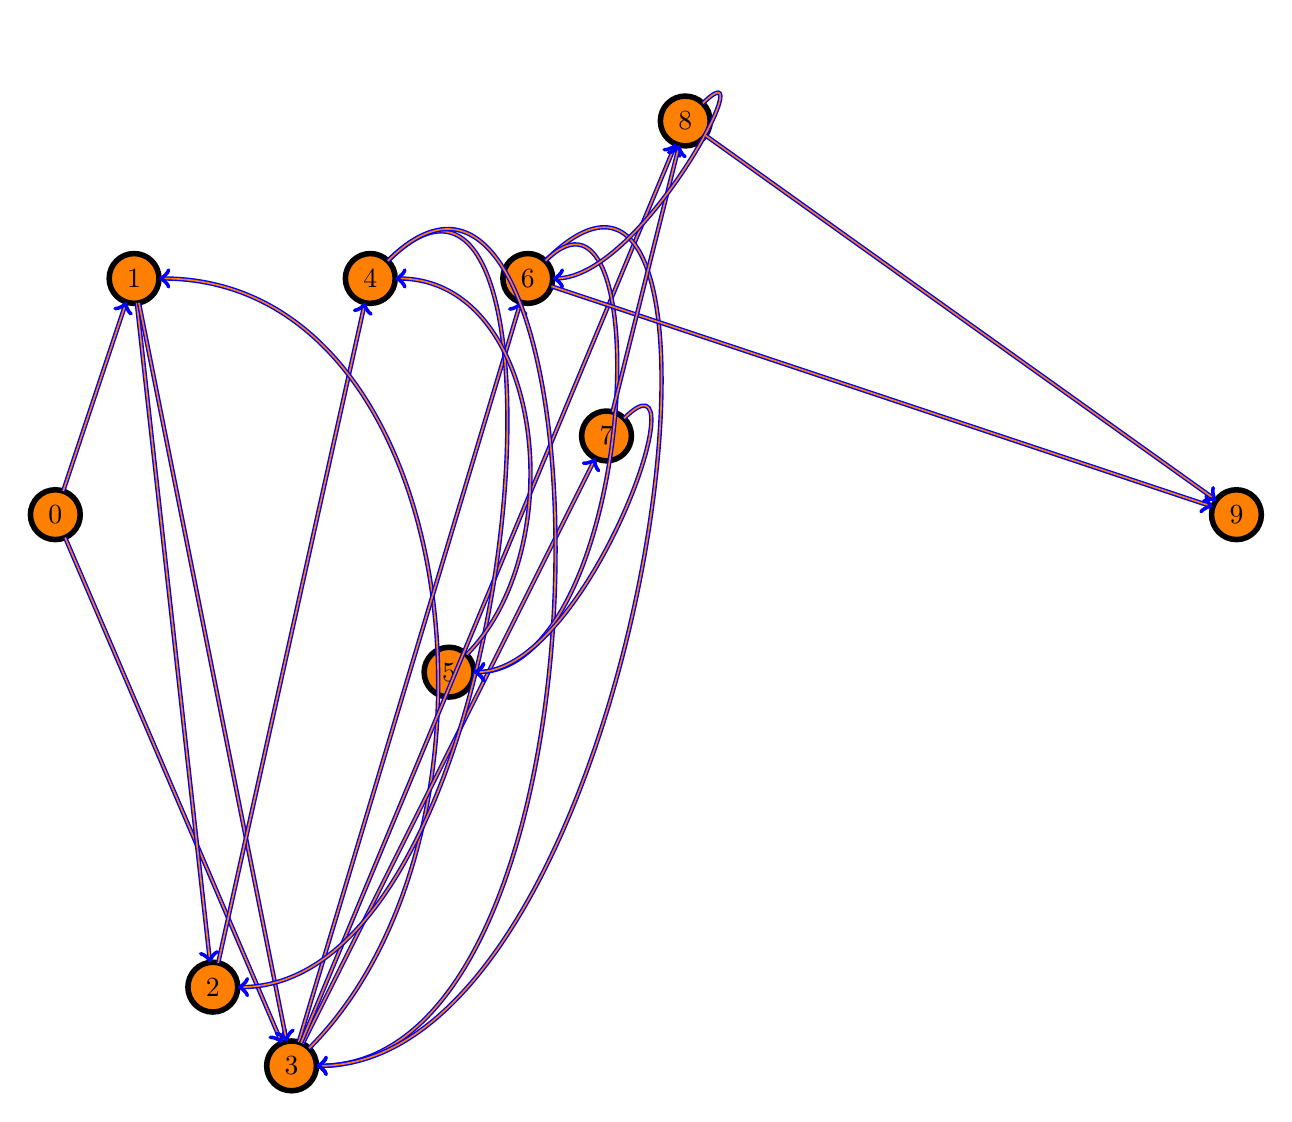
\begin{tikzpicture}
\SetVertexNormal[Shape      = circle,
FillColor  = orange,
LineWidth  = 2pt]
\SetUpEdge[lw         = 0.5pt,
color      = black,
labelcolor = white,
labeltext  = red,
labelstyle = {sloped,text=blue}]
\tikzstyle{TempStyle}=[double = orange]
\Vertex[x=-10, y=8]{0}
\Vertex[x=-9, y=11]{1}
\Vertex[x=-8, y=2]{2}
\Vertex[x=-7, y=1]{3}
\Vertex[x=-6, y=11]{4}
\Vertex[x=-5, y=6]{5}
\Vertex[x=-4, y=11]{6}
\Vertex[x=-3, y=9]{7}
\Vertex[x=-2, y=13]{8}
\Vertex[x=5, y=8]{9}
\tikzset{EdgeStyle/.style={->,TempStyle,relative=false,right=60,color=blue}}
\Edge(0)(1)
\tikzset{EdgeStyle/.style={->,TempStyle,relative=false,right=60,color=blue}}
\Edge(0)(3)
\tikzset{EdgeStyle/.style={->,TempStyle,relative=false,right=60,color=blue}}
\Edge(1)(2)
\tikzset{EdgeStyle/.style={->,TempStyle,relative=false,right=60,color=blue}}
\Edge(1)(3)
\tikzset{EdgeStyle/.style={->,TempStyle,relative=false,right=60,color=blue}}
\Edge(2)(4)
\tikzset{EdgeStyle/.style={->,TempStyle,relative=false,left=60,color=blue,in=0,draw}}
\Edge(3)(1)
\tikzset{EdgeStyle/.style={->,TempStyle,relative=false,right=60,color=blue}}
\Edge(3)(6)
\tikzset{EdgeStyle/.style={->,TempStyle,relative=false,right=60,color=blue}}
\Edge(3)(7)
\tikzset{EdgeStyle/.style={->,TempStyle,relative=false,right=60,color=blue}}
\Edge(3)(8)
\tikzset{EdgeStyle/.style={->,TempStyle,relative=false,left=60,color=blue,in=0,draw}}
\Edge(4)(2)
\tikzset{EdgeStyle/.style={->,TempStyle,relative=false,left=60,color=blue,in=0,draw}}
\Edge(4)(3)
\tikzset{EdgeStyle/.style={->,TempStyle,relative=false,left=60,color=blue,in=0,draw}}
\Edge(5)(4)
\tikzset{EdgeStyle/.style={->,TempStyle,relative=false,left=60,color=blue,in=0,draw}}
\Edge(6)(3)
\tikzset{EdgeStyle/.style={->,TempStyle,relative=false,left=60,color=blue,in=0,draw}}
\Edge(6)(5)
\tikzset{EdgeStyle/.style={->,TempStyle,relative=false,right=60,color=blue}}
\Edge(6)(9)
\tikzset{EdgeStyle/.style={->,TempStyle,relative=false,left=60,color=blue,in=0,draw}}
\Edge(7)(5)
\tikzset{EdgeStyle/.style={->,TempStyle,relative=false,right=60,color=blue}}
\Edge(7)(8)
\tikzset{EdgeStyle/.style={->,TempStyle,relative=false,left=60,color=blue,in=0,draw}}
\Edge(8)(6)
\tikzset{EdgeStyle/.style={->,TempStyle,relative=false,right=60,color=blue}}
\Edge(8)(9)
\end{tikzpicture}\\
\begin{center}\begin{tabular}{l c}\\
\textcolor{orange}{\LARGE$\rightarrow$} & Chemin \\
 \textcolor{red}{\LARGE$\rightarrow$} & Créations arcs\\
 \textcolor{green}{\LARGE$\rightarrow$} & Modification flot\\
\end{tabular}
\end{center}
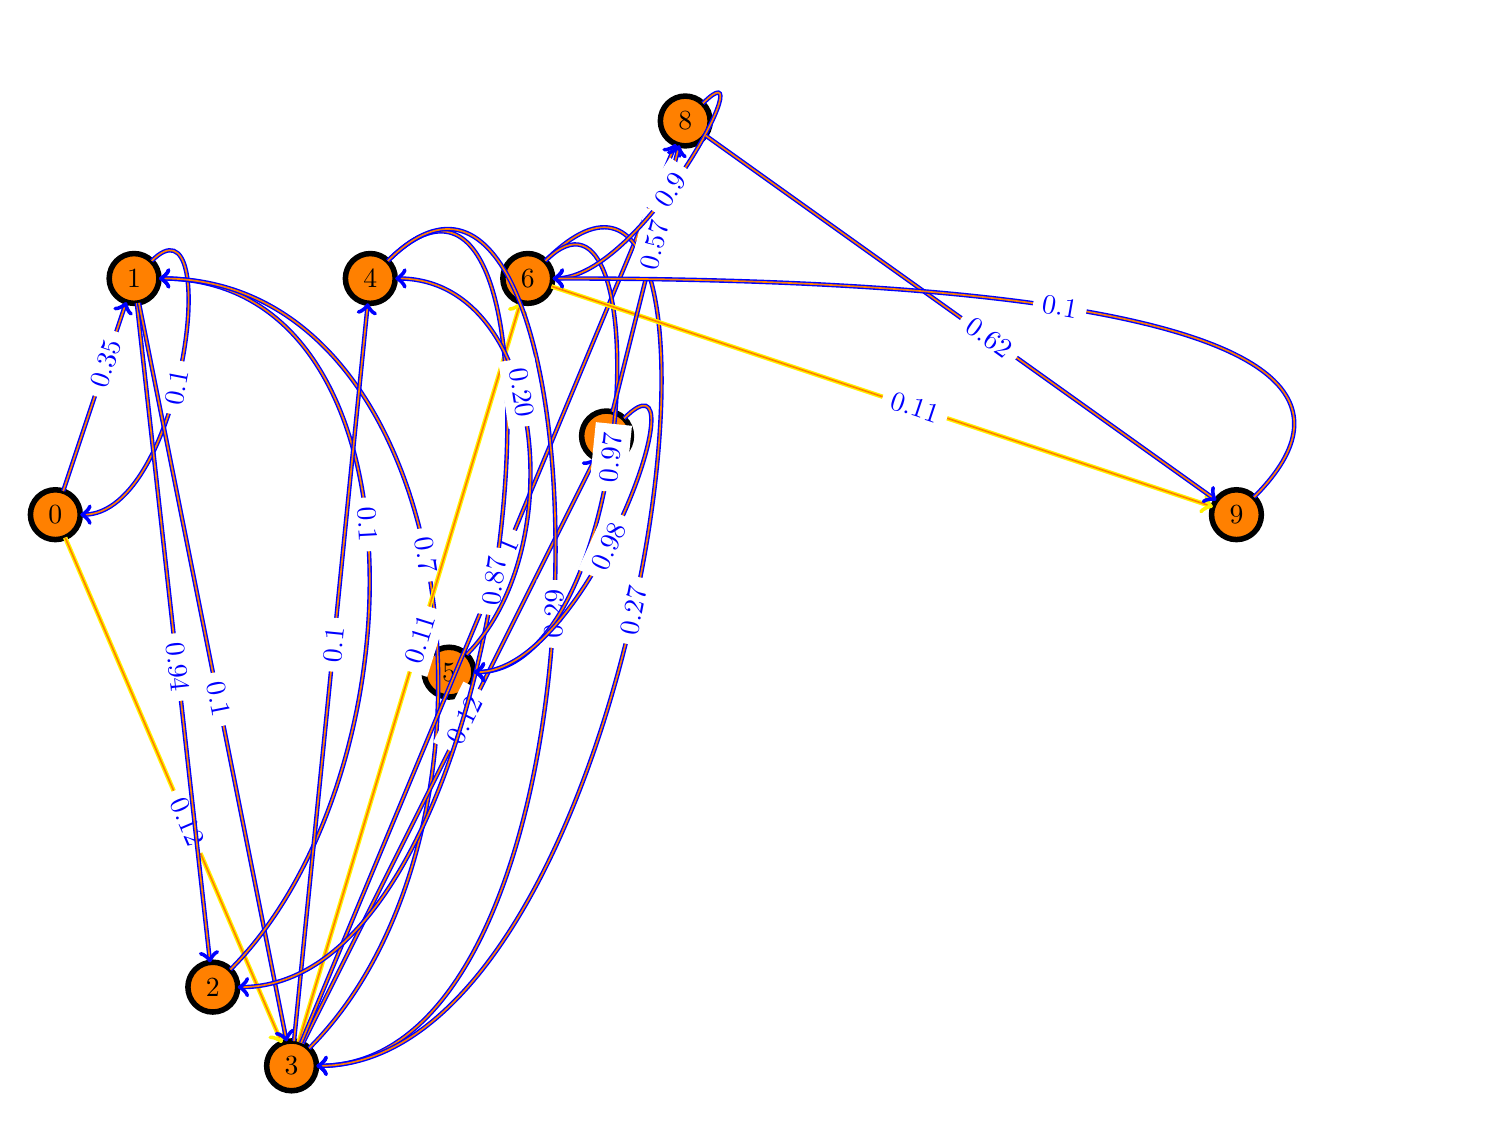
\begin{tikzpicture}
\SetVertexNormal[Shape      = circle,
FillColor  = orange,
LineWidth  = 2pt]
\SetUpEdge[lw         = 0.5pt,
color      = black,
labelcolor = white,
labeltext  = red,
labelstyle = {sloped,text=blue}]
\tikzstyle{TempStyle}=[double = orange]
\Vertex[x=-10, y=8]{0}
\Vertex[x=-9, y=11]{1}
\Vertex[x=-8, y=2]{2}
\Vertex[x=-7, y=1]{3}
\Vertex[x=-6, y=11]{4}
\Vertex[x=-5, y=6]{5}
\Vertex[x=-4, y=11]{6}
\Vertex[x=-3, y=9]{7}
\Vertex[x=-2, y=13]{8}
\Vertex[x=5, y=8]{9}
\tikzset{EdgeStyle/.style={->,TempStyle,relative=false,right=60,color=blue}}
\Edge[label=$0.35$](0)(1)
\tikzset{EdgeStyle/.style={->,TempStyle,relative=false,right=60,color=yellow}}
\Edge[label=$0.12$](0)(3)
\tikzset{EdgeStyle/.style={->,TempStyle,relative=false,left=60,color=blue,in=0,draw}}
\Edge[label=$0.1$](1)(0)
\tikzset{EdgeStyle/.style={->,TempStyle,relative=false,right=60,color=blue}}
\Edge[label=$0.94$](1)(2)
\tikzset{EdgeStyle/.style={->,TempStyle,relative=false,right=60,color=blue}}
\Edge[label=$0.1$](1)(3)
\tikzset{EdgeStyle/.style={->,TempStyle,relative=false,left=60,color=blue,in=0,draw}}
\Edge[label=$0.1$](2)(1)
\tikzset{EdgeStyle/.style={->,TempStyle,relative=false,left=60,color=blue,in=0,draw}}
\Edge[label=$0.7$](3)(1)
\tikzset{EdgeStyle/.style={->,TempStyle,relative=false,right=60,color=blue}}
\Edge[label=$0.1$](3)(4)
\tikzset{EdgeStyle/.style={->,TempStyle,relative=false,right=60,color=yellow}}
\Edge[label=$0.11$](3)(6)
\tikzset{EdgeStyle/.style={->,TempStyle,relative=false,right=60,color=blue}}
\Edge[label=$0.12$](3)(7)
\tikzset{EdgeStyle/.style={->,TempStyle,relative=false,right=60,color=blue}}
\Edge[label=$0.61$](3)(8)
\tikzset{EdgeStyle/.style={->,TempStyle,relative=false,left=60,color=blue,in=0,draw}}
\Edge[label=$0.87$](4)(2)
\tikzset{EdgeStyle/.style={->,TempStyle,relative=false,left=60,color=blue,in=0,draw}}
\Edge[label=$0.29$](4)(3)
\tikzset{EdgeStyle/.style={->,TempStyle,relative=false,left=60,color=blue,in=0,draw}}
\Edge[label=$0.20$](5)(4)
\tikzset{EdgeStyle/.style={->,TempStyle,relative=false,left=60,color=blue,in=0,draw}}
\Edge[label=$0.27$](6)(3)
\tikzset{EdgeStyle/.style={->,TempStyle,relative=false,left=60,color=blue,in=0,draw}}
\Edge[label=$0.97$](6)(5)
\tikzset{EdgeStyle/.style={->,TempStyle,relative=false,right=60,color=yellow}}
\Edge[label=$0.11$](6)(9)
\tikzset{EdgeStyle/.style={->,TempStyle,relative=false,left=60,color=blue,in=0,draw}}
\Edge[label=$0.98$](7)(5)
\tikzset{EdgeStyle/.style={->,TempStyle,relative=false,right=60,color=blue}}
\Edge[label=$0.57$](7)(8)
\tikzset{EdgeStyle/.style={->,TempStyle,relative=false,left=60,color=blue,in=0,draw}}
\Edge[label=$0.9$](8)(6)
\tikzset{EdgeStyle/.style={->,TempStyle,relative=false,right=60,color=blue}}
\Edge[label=$0.62$](8)(9)
\tikzset{EdgeStyle/.style={->,TempStyle,relative=false,left=60,color=blue,in=0,draw}}
\Edge[label=$0.1$](9)(6)
\end{tikzpicture}\\
\begin{center}\begin{tabular}{l c}\\
\textcolor{orange}{\LARGE$\rightarrow$} & Chemin \\
 \textcolor{red}{\LARGE$\rightarrow$} & Créations arcs\\
 \textcolor{green}{\LARGE$\rightarrow$} & Modification flot\\
\end{tabular}
\end{center}
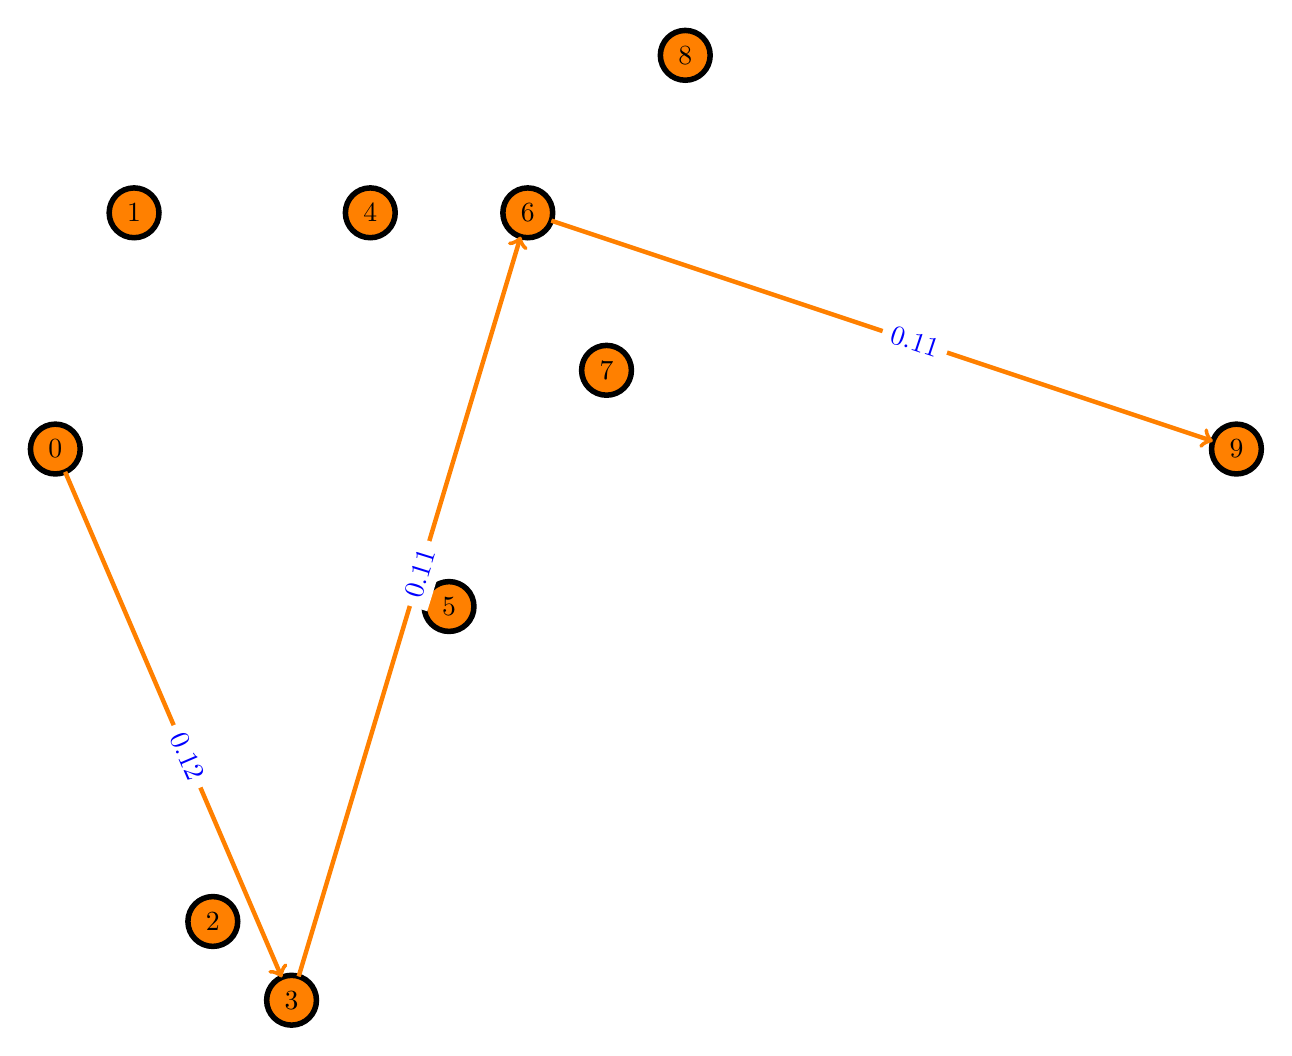
\begin{tikzpicture}
\SetVertexNormal[Shape      = circle,
FillColor  = orange,
LineWidth  = 2pt]
\SetUpEdge[lw         = 0.5pt,
color      = black,
labelcolor = white,
labeltext  = red,
labelstyle = {sloped,text=blue}]
\tikzstyle{TempStyle}=[double = orange]
\Vertex[x=-10, y=8]{0}
\Vertex[x=-9, y=11]{1}
\Vertex[x=-8, y=2]{2}
\Vertex[x=-7, y=1]{3}
\Vertex[x=-6, y=11]{4}
\Vertex[x=-5, y=6]{5}
\Vertex[x=-4, y=11]{6}
\Vertex[x=-3, y=9]{7}
\Vertex[x=-2, y=13]{8}
\Vertex[x=5, y=8]{9}
\tikzset{EdgeStyle/.style={->,TempStyle,relative=false,right=60,color=orange}}
\Edge[label=$0.12$](0)(3)
\tikzset{EdgeStyle/.style={->,TempStyle,relative=false,right=60,color=orange}}
\Edge[label=$0.11$](3)(6)
\tikzset{EdgeStyle/.style={->,TempStyle,relative=false,right=60,color=orange}}
\Edge[label=$0.11$](6)(9)
\end{tikzpicture}\\
\begin{center}\begin{tabular}{l c}\\
\textcolor{orange}{\LARGE$\rightarrow$} & Chemin \\
 \textcolor{red}{\LARGE$\rightarrow$} & Créations arcs\\
 \textcolor{green}{\LARGE$\rightarrow$} & Modification flot\\
\end{tabular}
\end{center}
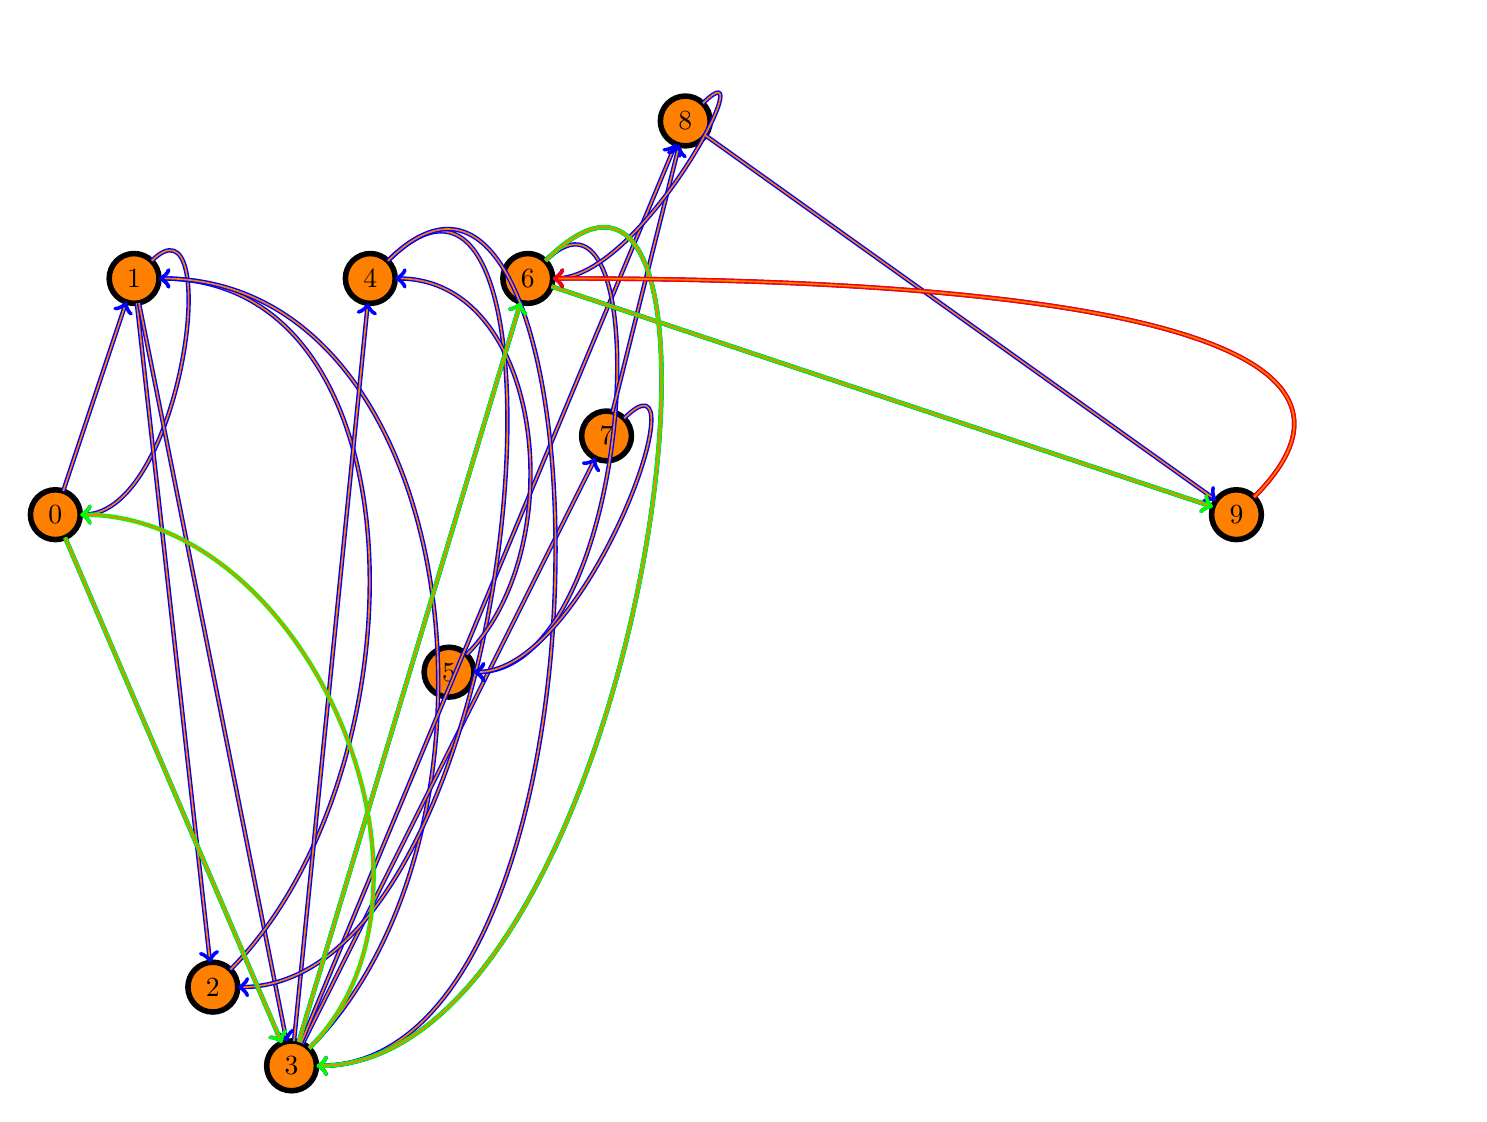
\begin{tikzpicture}
\SetVertexNormal[Shape      = circle,
FillColor  = orange,
LineWidth  = 2pt]
\SetUpEdge[lw         = 0.5pt,
color      = black,
labelcolor = white,
labeltext  = red,
labelstyle = {sloped,text=blue}]
\tikzstyle{TempStyle}=[double = orange]
\Vertex[x=-10, y=8]{0}
\Vertex[x=-9, y=11]{1}
\Vertex[x=-8, y=2]{2}
\Vertex[x=-7, y=1]{3}
\Vertex[x=-6, y=11]{4}
\Vertex[x=-5, y=6]{5}
\Vertex[x=-4, y=11]{6}
\Vertex[x=-3, y=9]{7}
\Vertex[x=-2, y=13]{8}
\Vertex[x=5, y=8]{9}
\tikzset{EdgeStyle/.style={->,TempStyle,relative=false,right=60,color=blue}}
\Edge(0)(1)
\tikzset{EdgeStyle/.style={->,TempStyle,relative=false,right=60,color=blue}}
\Edge(0)(3)
\tikzset{EdgeStyle/.style={->,TempStyle,relative=false,left=60,color=blue,in=0,draw}}
\Edge(1)(0)
\tikzset{EdgeStyle/.style={->,TempStyle,relative=false,right=60,color=blue}}
\Edge(1)(2)
\tikzset{EdgeStyle/.style={->,TempStyle,relative=false,right=60,color=blue}}
\Edge(1)(3)
\tikzset{EdgeStyle/.style={->,TempStyle,relative=false,left=60,color=blue,in=0,draw}}
\Edge(2)(1)
\tikzset{EdgeStyle/.style={->,TempStyle,relative=false,left=60,color=blue,in=0,draw}}
\Edge(3)(1)
\tikzset{EdgeStyle/.style={->,TempStyle,relative=false,right=60,color=blue}}
\Edge(3)(4)
\tikzset{EdgeStyle/.style={->,TempStyle,relative=false,right=60,color=blue}}
\Edge(3)(6)
\tikzset{EdgeStyle/.style={->,TempStyle,relative=false,right=60,color=blue}}
\Edge(3)(7)
\tikzset{EdgeStyle/.style={->,TempStyle,relative=false,right=60,color=blue}}
\Edge(3)(8)
\tikzset{EdgeStyle/.style={->,TempStyle,relative=false,left=60,color=blue,in=0,draw}}
\Edge(4)(2)
\tikzset{EdgeStyle/.style={->,TempStyle,relative=false,left=60,color=blue,in=0,draw}}
\Edge(4)(3)
\tikzset{EdgeStyle/.style={->,TempStyle,relative=false,left=60,color=blue,in=0,draw}}
\Edge(5)(4)
\tikzset{EdgeStyle/.style={->,TempStyle,relative=false,left=60,color=blue,in=0,draw}}
\Edge(6)(3)
\tikzset{EdgeStyle/.style={->,TempStyle,relative=false,left=60,color=blue,in=0,draw}}
\Edge(6)(5)
\tikzset{EdgeStyle/.style={->,TempStyle,relative=false,right=60,color=blue}}
\Edge(6)(9)
\tikzset{EdgeStyle/.style={->,TempStyle,relative=false,left=60,color=blue,in=0,draw}}
\Edge(7)(5)
\tikzset{EdgeStyle/.style={->,TempStyle,relative=false,right=60,color=blue}}
\Edge(7)(8)
\tikzset{EdgeStyle/.style={->,TempStyle,relative=false,left=60,color=blue,in=0,draw}}
\Edge(8)(6)
\tikzset{EdgeStyle/.style={->,TempStyle,relative=false,right=60,color=blue}}
\Edge(8)(9)
\tikzset{EdgeStyle/.style={->,TempStyle,relative=false,left=60,color=blue,in=0,draw}}
\Edge(9)(6)
\tikzset{EdgeStyle/.style={->,TempStyle,relative=false,right=60,color=green}}
\Edge(0)(3)
\tikzset{EdgeStyle/.style={->,TempStyle,relative=false,right=60,in=0,color=green}}
\Edge(3)(0)
\tikzset{EdgeStyle/.style={->,TempStyle,relative=false,right=60,color=green}}
\Edge(3)(6)
\tikzset{EdgeStyle/.style={->,TempStyle,relative=false,right=60,in=0,color=green}}
\Edge(6)(3)
\tikzset{EdgeStyle/.style={->,TempStyle,relative=false,right=60,color=green}}
\Edge(6)(9)
\tikzset{EdgeStyle/.style={->,TempStyle,relative=false,right=60,in=0,color=red}}
\Edge(9)(6)
\end{tikzpicture}\\
\begin{center}\begin{tabular}{l c}\\
\textcolor{orange}{\LARGE$\rightarrow$} & Chemin \\
 \textcolor{red}{\LARGE$\rightarrow$} & Créations arcs\\
 \textcolor{green}{\LARGE$\rightarrow$} & Modification flot\\
\end{tabular}
\end{center}
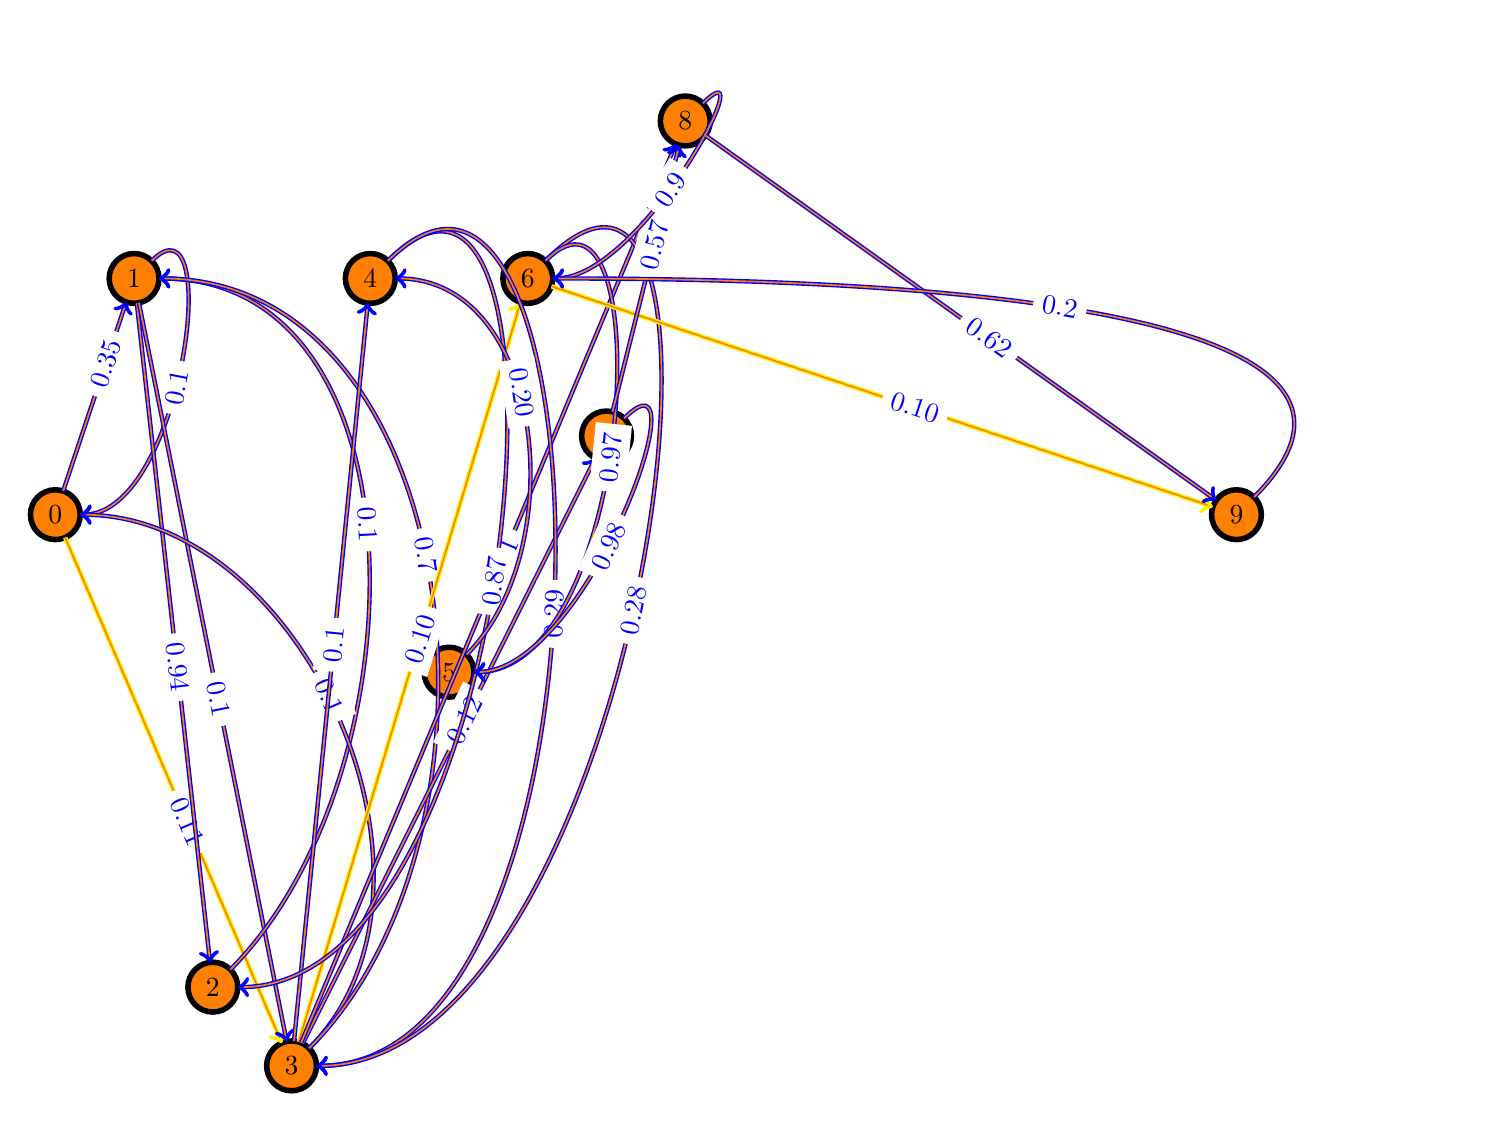
\begin{tikzpicture}
\SetVertexNormal[Shape      = circle,
FillColor  = orange,
LineWidth  = 2pt]
\SetUpEdge[lw         = 0.5pt,
color      = black,
labelcolor = white,
labeltext  = red,
labelstyle = {sloped,text=blue}]
\tikzstyle{TempStyle}=[double = orange]
\Vertex[x=-10, y=8]{0}
\Vertex[x=-9, y=11]{1}
\Vertex[x=-8, y=2]{2}
\Vertex[x=-7, y=1]{3}
\Vertex[x=-6, y=11]{4}
\Vertex[x=-5, y=6]{5}
\Vertex[x=-4, y=11]{6}
\Vertex[x=-3, y=9]{7}
\Vertex[x=-2, y=13]{8}
\Vertex[x=5, y=8]{9}
\tikzset{EdgeStyle/.style={->,TempStyle,relative=false,right=60,color=blue}}
\Edge[label=$0.35$](0)(1)
\tikzset{EdgeStyle/.style={->,TempStyle,relative=false,right=60,color=yellow}}
\Edge[label=$0.11$](0)(3)
\tikzset{EdgeStyle/.style={->,TempStyle,relative=false,left=60,color=blue,in=0,draw}}
\Edge[label=$0.1$](1)(0)
\tikzset{EdgeStyle/.style={->,TempStyle,relative=false,right=60,color=blue}}
\Edge[label=$0.94$](1)(2)
\tikzset{EdgeStyle/.style={->,TempStyle,relative=false,right=60,color=blue}}
\Edge[label=$0.1$](1)(3)
\tikzset{EdgeStyle/.style={->,TempStyle,relative=false,left=60,color=blue,in=0,draw}}
\Edge[label=$0.1$](2)(1)
\tikzset{EdgeStyle/.style={->,TempStyle,relative=false,left=60,color=blue,in=0,draw}}
\Edge[label=$0.1$](3)(0)
\tikzset{EdgeStyle/.style={->,TempStyle,relative=false,left=60,color=blue,in=0,draw}}
\Edge[label=$0.7$](3)(1)
\tikzset{EdgeStyle/.style={->,TempStyle,relative=false,right=60,color=blue}}
\Edge[label=$0.1$](3)(4)
\tikzset{EdgeStyle/.style={->,TempStyle,relative=false,right=60,color=yellow}}
\Edge[label=$0.10$](3)(6)
\tikzset{EdgeStyle/.style={->,TempStyle,relative=false,right=60,color=blue}}
\Edge[label=$0.12$](3)(7)
\tikzset{EdgeStyle/.style={->,TempStyle,relative=false,right=60,color=blue}}
\Edge[label=$0.61$](3)(8)
\tikzset{EdgeStyle/.style={->,TempStyle,relative=false,left=60,color=blue,in=0,draw}}
\Edge[label=$0.87$](4)(2)
\tikzset{EdgeStyle/.style={->,TempStyle,relative=false,left=60,color=blue,in=0,draw}}
\Edge[label=$0.29$](4)(3)
\tikzset{EdgeStyle/.style={->,TempStyle,relative=false,left=60,color=blue,in=0,draw}}
\Edge[label=$0.20$](5)(4)
\tikzset{EdgeStyle/.style={->,TempStyle,relative=false,left=60,color=blue,in=0,draw}}
\Edge[label=$0.28$](6)(3)
\tikzset{EdgeStyle/.style={->,TempStyle,relative=false,left=60,color=blue,in=0,draw}}
\Edge[label=$0.97$](6)(5)
\tikzset{EdgeStyle/.style={->,TempStyle,relative=false,right=60,color=yellow}}
\Edge[label=$0.10$](6)(9)
\tikzset{EdgeStyle/.style={->,TempStyle,relative=false,left=60,color=blue,in=0,draw}}
\Edge[label=$0.98$](7)(5)
\tikzset{EdgeStyle/.style={->,TempStyle,relative=false,right=60,color=blue}}
\Edge[label=$0.57$](7)(8)
\tikzset{EdgeStyle/.style={->,TempStyle,relative=false,left=60,color=blue,in=0,draw}}
\Edge[label=$0.9$](8)(6)
\tikzset{EdgeStyle/.style={->,TempStyle,relative=false,right=60,color=blue}}
\Edge[label=$0.62$](8)(9)
\tikzset{EdgeStyle/.style={->,TempStyle,relative=false,left=60,color=blue,in=0,draw}}
\Edge[label=$0.2$](9)(6)
\end{tikzpicture}\\
\begin{center}\begin{tabular}{l c}\\
\textcolor{orange}{\LARGE$\rightarrow$} & Chemin \\
 \textcolor{red}{\LARGE$\rightarrow$} & Créations arcs\\
 \textcolor{green}{\LARGE$\rightarrow$} & Modification flot\\
\end{tabular}
\end{center}
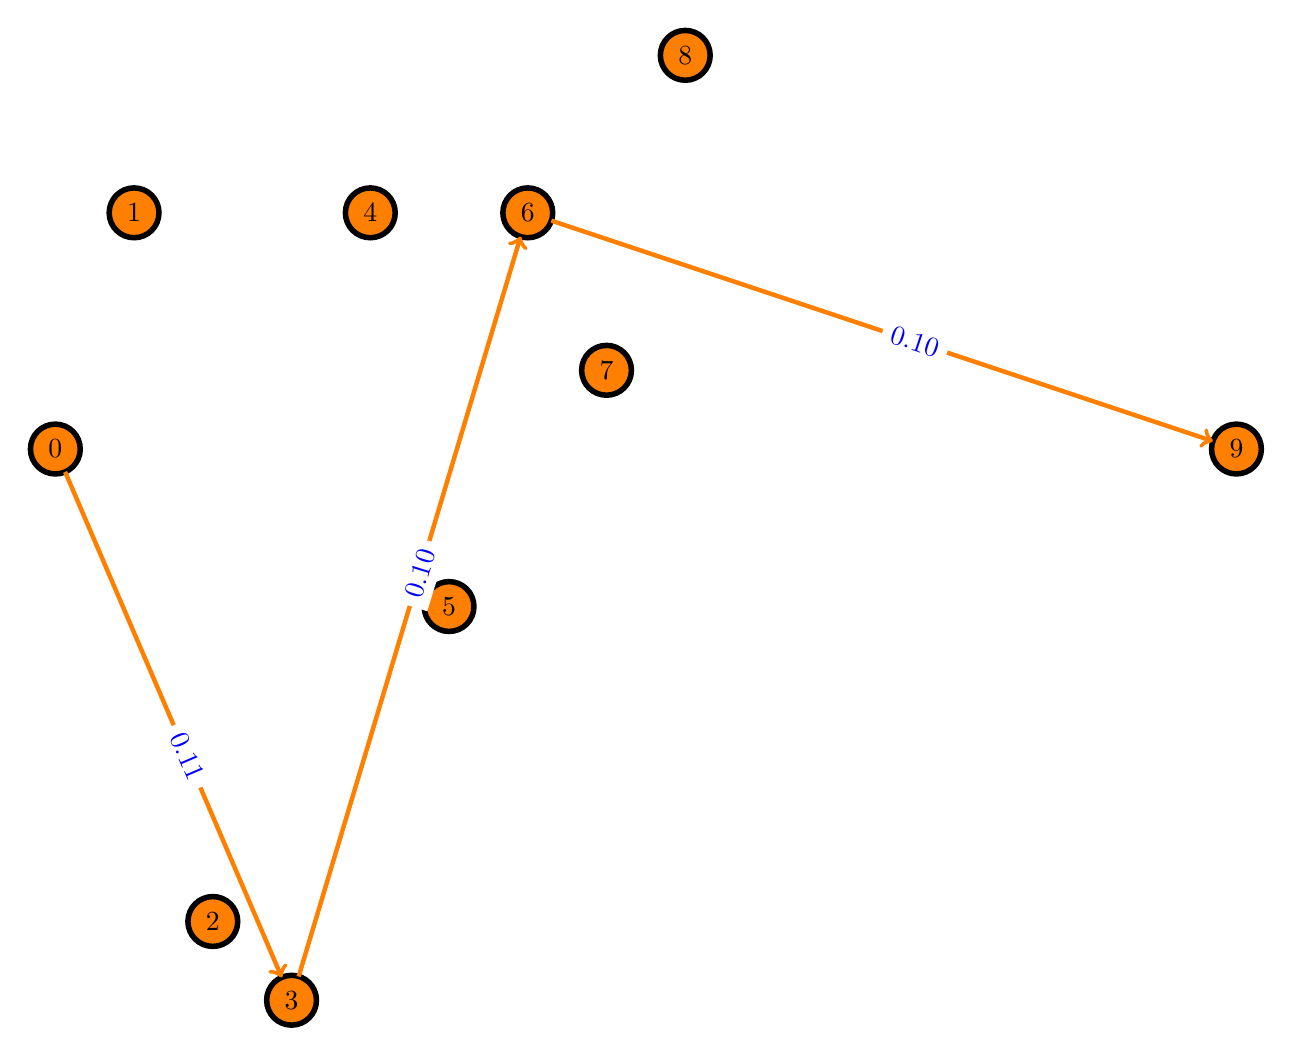
\begin{tikzpicture}
\SetVertexNormal[Shape      = circle,
FillColor  = orange,
LineWidth  = 2pt]
\SetUpEdge[lw         = 0.5pt,
color      = black,
labelcolor = white,
labeltext  = red,
labelstyle = {sloped,text=blue}]
\tikzstyle{TempStyle}=[double = orange]
\Vertex[x=-10, y=8]{0}
\Vertex[x=-9, y=11]{1}
\Vertex[x=-8, y=2]{2}
\Vertex[x=-7, y=1]{3}
\Vertex[x=-6, y=11]{4}
\Vertex[x=-5, y=6]{5}
\Vertex[x=-4, y=11]{6}
\Vertex[x=-3, y=9]{7}
\Vertex[x=-2, y=13]{8}
\Vertex[x=5, y=8]{9}
\tikzset{EdgeStyle/.style={->,TempStyle,relative=false,right=60,color=orange}}
\Edge[label=$0.11$](0)(3)
\tikzset{EdgeStyle/.style={->,TempStyle,relative=false,right=60,color=orange}}
\Edge[label=$0.10$](3)(6)
\tikzset{EdgeStyle/.style={->,TempStyle,relative=false,right=60,color=orange}}
\Edge[label=$0.10$](6)(9)
\end{tikzpicture}\\
\begin{center}\begin{tabular}{l c}\\
\textcolor{orange}{\LARGE$\rightarrow$} & Chemin \\
 \textcolor{red}{\LARGE$\rightarrow$} & Créations arcs\\
 \textcolor{green}{\LARGE$\rightarrow$} & Modification flot\\
\end{tabular}
\end{center}
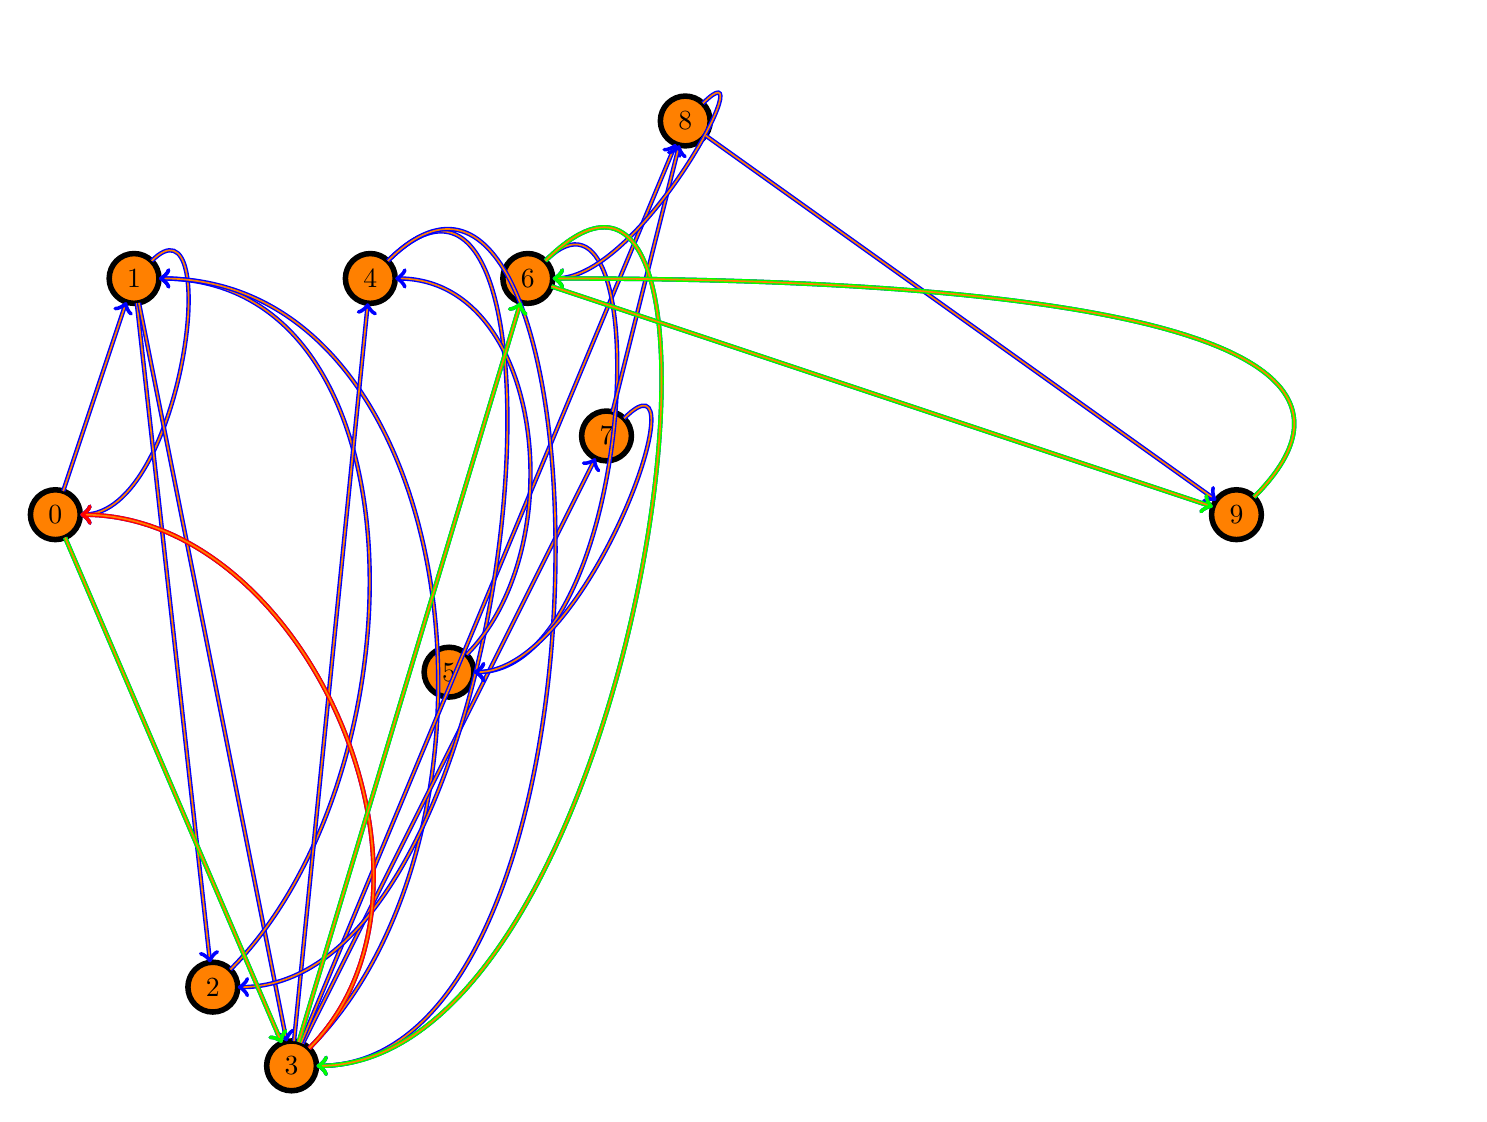
\begin{tikzpicture}
\SetVertexNormal[Shape      = circle,
FillColor  = orange,
LineWidth  = 2pt]
\SetUpEdge[lw         = 0.5pt,
color      = black,
labelcolor = white,
labeltext  = red,
labelstyle = {sloped,text=blue}]
\tikzstyle{TempStyle}=[double = orange]
\Vertex[x=-10, y=8]{0}
\Vertex[x=-9, y=11]{1}
\Vertex[x=-8, y=2]{2}
\Vertex[x=-7, y=1]{3}
\Vertex[x=-6, y=11]{4}
\Vertex[x=-5, y=6]{5}
\Vertex[x=-4, y=11]{6}
\Vertex[x=-3, y=9]{7}
\Vertex[x=-2, y=13]{8}
\Vertex[x=5, y=8]{9}
\tikzset{EdgeStyle/.style={->,TempStyle,relative=false,right=60,color=blue}}
\Edge(0)(1)
\tikzset{EdgeStyle/.style={->,TempStyle,relative=false,right=60,color=blue}}
\Edge(0)(3)
\tikzset{EdgeStyle/.style={->,TempStyle,relative=false,left=60,color=blue,in=0,draw}}
\Edge(1)(0)
\tikzset{EdgeStyle/.style={->,TempStyle,relative=false,right=60,color=blue}}
\Edge(1)(2)
\tikzset{EdgeStyle/.style={->,TempStyle,relative=false,right=60,color=blue}}
\Edge(1)(3)
\tikzset{EdgeStyle/.style={->,TempStyle,relative=false,left=60,color=blue,in=0,draw}}
\Edge(2)(1)
\tikzset{EdgeStyle/.style={->,TempStyle,relative=false,left=60,color=blue,in=0,draw}}
\Edge(3)(0)
\tikzset{EdgeStyle/.style={->,TempStyle,relative=false,left=60,color=blue,in=0,draw}}
\Edge(3)(1)
\tikzset{EdgeStyle/.style={->,TempStyle,relative=false,right=60,color=blue}}
\Edge(3)(4)
\tikzset{EdgeStyle/.style={->,TempStyle,relative=false,right=60,color=blue}}
\Edge(3)(6)
\tikzset{EdgeStyle/.style={->,TempStyle,relative=false,right=60,color=blue}}
\Edge(3)(7)
\tikzset{EdgeStyle/.style={->,TempStyle,relative=false,right=60,color=blue}}
\Edge(3)(8)
\tikzset{EdgeStyle/.style={->,TempStyle,relative=false,left=60,color=blue,in=0,draw}}
\Edge(4)(2)
\tikzset{EdgeStyle/.style={->,TempStyle,relative=false,left=60,color=blue,in=0,draw}}
\Edge(4)(3)
\tikzset{EdgeStyle/.style={->,TempStyle,relative=false,left=60,color=blue,in=0,draw}}
\Edge(5)(4)
\tikzset{EdgeStyle/.style={->,TempStyle,relative=false,left=60,color=blue,in=0,draw}}
\Edge(6)(3)
\tikzset{EdgeStyle/.style={->,TempStyle,relative=false,left=60,color=blue,in=0,draw}}
\Edge(6)(5)
\tikzset{EdgeStyle/.style={->,TempStyle,relative=false,right=60,color=blue}}
\Edge(6)(9)
\tikzset{EdgeStyle/.style={->,TempStyle,relative=false,left=60,color=blue,in=0,draw}}
\Edge(7)(5)
\tikzset{EdgeStyle/.style={->,TempStyle,relative=false,right=60,color=blue}}
\Edge(7)(8)
\tikzset{EdgeStyle/.style={->,TempStyle,relative=false,left=60,color=blue,in=0,draw}}
\Edge(8)(6)
\tikzset{EdgeStyle/.style={->,TempStyle,relative=false,right=60,color=blue}}
\Edge(8)(9)
\tikzset{EdgeStyle/.style={->,TempStyle,relative=false,left=60,color=blue,in=0,draw}}
\Edge(9)(6)
\tikzset{EdgeStyle/.style={->,TempStyle,relative=false,right=60,color=green}}
\Edge(0)(3)
\tikzset{EdgeStyle/.style={->,TempStyle,relative=false,right=60,in=0,color=red}}
\Edge(3)(0)
\tikzset{EdgeStyle/.style={->,TempStyle,relative=false,right=60,color=green}}
\Edge(3)(6)
\tikzset{EdgeStyle/.style={->,TempStyle,relative=false,right=60,in=0,color=green}}
\Edge(6)(3)
\tikzset{EdgeStyle/.style={->,TempStyle,relative=false,right=60,color=green}}
\Edge(6)(9)
\tikzset{EdgeStyle/.style={->,TempStyle,relative=false,right=60,in=0,color=green}}
\Edge(9)(6)
\end{tikzpicture}\\
\begin{center}\begin{tabular}{l c}\\
\textcolor{orange}{\LARGE$\rightarrow$} & Chemin \\
 \textcolor{red}{\LARGE$\rightarrow$} & Créations arcs\\
 \textcolor{green}{\LARGE$\rightarrow$} & Modification flot\\
\end{tabular}
\end{center}
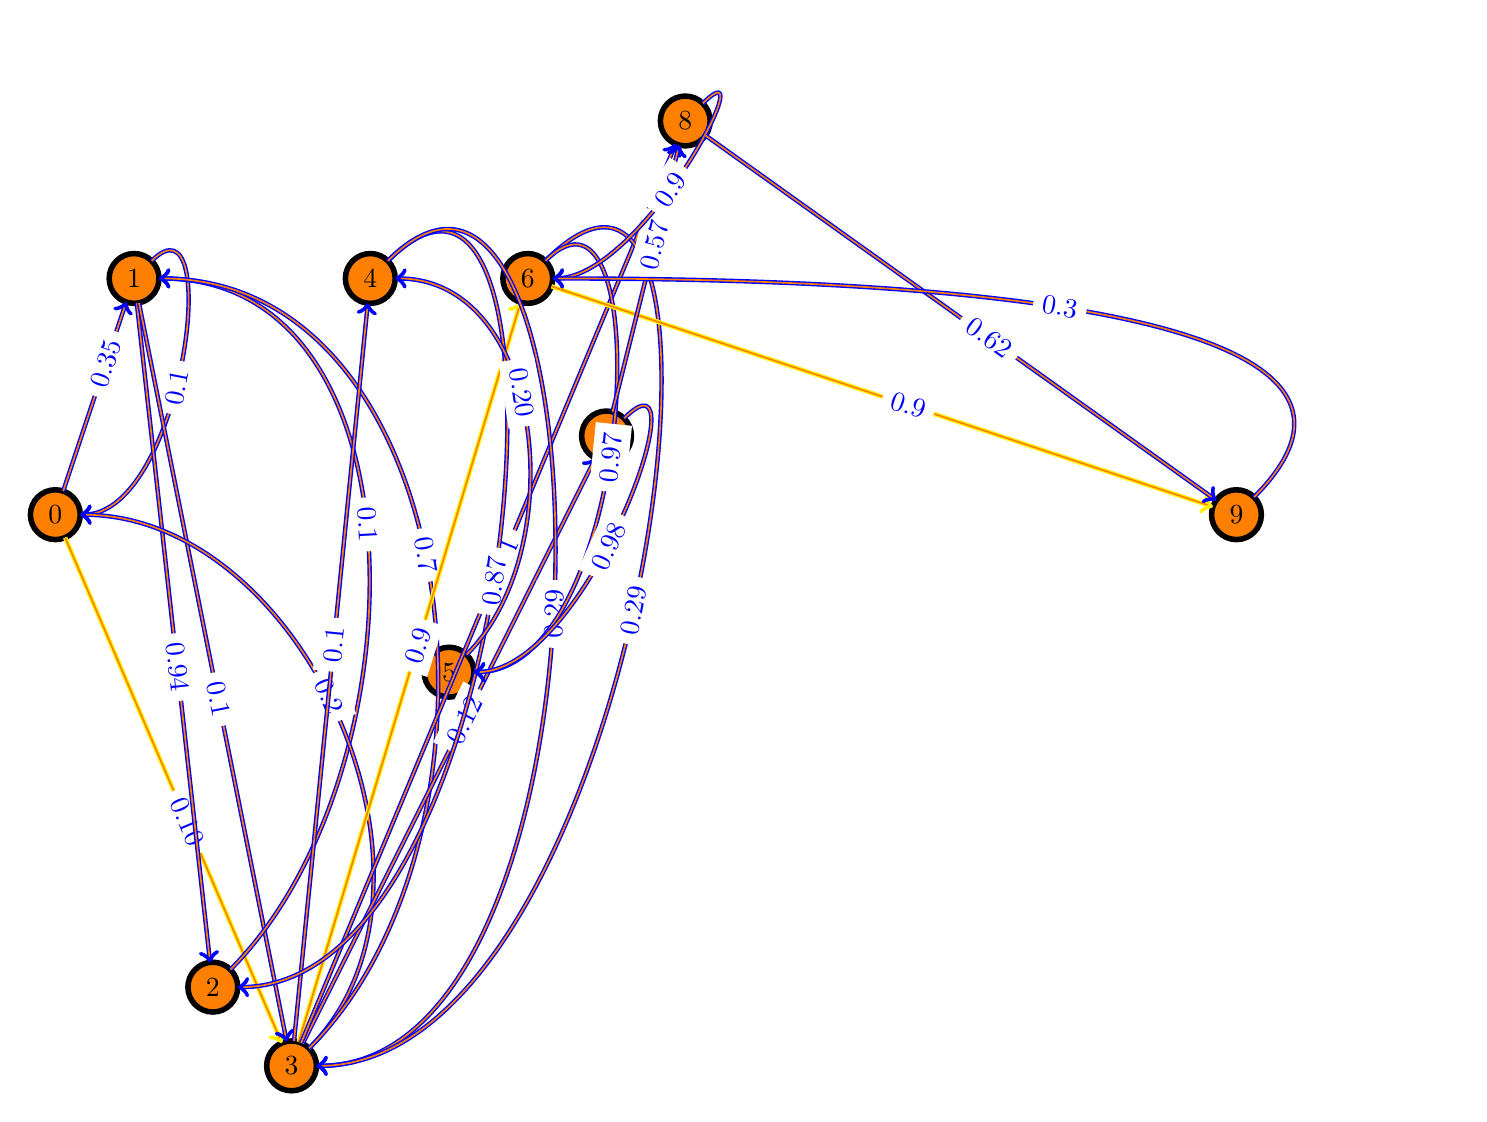
\begin{tikzpicture}
\SetVertexNormal[Shape      = circle,
FillColor  = orange,
LineWidth  = 2pt]
\SetUpEdge[lw         = 0.5pt,
color      = black,
labelcolor = white,
labeltext  = red,
labelstyle = {sloped,text=blue}]
\tikzstyle{TempStyle}=[double = orange]
\Vertex[x=-10, y=8]{0}
\Vertex[x=-9, y=11]{1}
\Vertex[x=-8, y=2]{2}
\Vertex[x=-7, y=1]{3}
\Vertex[x=-6, y=11]{4}
\Vertex[x=-5, y=6]{5}
\Vertex[x=-4, y=11]{6}
\Vertex[x=-3, y=9]{7}
\Vertex[x=-2, y=13]{8}
\Vertex[x=5, y=8]{9}
\tikzset{EdgeStyle/.style={->,TempStyle,relative=false,right=60,color=blue}}
\Edge[label=$0.35$](0)(1)
\tikzset{EdgeStyle/.style={->,TempStyle,relative=false,right=60,color=yellow}}
\Edge[label=$0.10$](0)(3)
\tikzset{EdgeStyle/.style={->,TempStyle,relative=false,left=60,color=blue,in=0,draw}}
\Edge[label=$0.1$](1)(0)
\tikzset{EdgeStyle/.style={->,TempStyle,relative=false,right=60,color=blue}}
\Edge[label=$0.94$](1)(2)
\tikzset{EdgeStyle/.style={->,TempStyle,relative=false,right=60,color=blue}}
\Edge[label=$0.1$](1)(3)
\tikzset{EdgeStyle/.style={->,TempStyle,relative=false,left=60,color=blue,in=0,draw}}
\Edge[label=$0.1$](2)(1)
\tikzset{EdgeStyle/.style={->,TempStyle,relative=false,left=60,color=blue,in=0,draw}}
\Edge[label=$0.2$](3)(0)
\tikzset{EdgeStyle/.style={->,TempStyle,relative=false,left=60,color=blue,in=0,draw}}
\Edge[label=$0.7$](3)(1)
\tikzset{EdgeStyle/.style={->,TempStyle,relative=false,right=60,color=blue}}
\Edge[label=$0.1$](3)(4)
\tikzset{EdgeStyle/.style={->,TempStyle,relative=false,right=60,color=yellow}}
\Edge[label=$0.9$](3)(6)
\tikzset{EdgeStyle/.style={->,TempStyle,relative=false,right=60,color=blue}}
\Edge[label=$0.12$](3)(7)
\tikzset{EdgeStyle/.style={->,TempStyle,relative=false,right=60,color=blue}}
\Edge[label=$0.61$](3)(8)
\tikzset{EdgeStyle/.style={->,TempStyle,relative=false,left=60,color=blue,in=0,draw}}
\Edge[label=$0.87$](4)(2)
\tikzset{EdgeStyle/.style={->,TempStyle,relative=false,left=60,color=blue,in=0,draw}}
\Edge[label=$0.29$](4)(3)
\tikzset{EdgeStyle/.style={->,TempStyle,relative=false,left=60,color=blue,in=0,draw}}
\Edge[label=$0.20$](5)(4)
\tikzset{EdgeStyle/.style={->,TempStyle,relative=false,left=60,color=blue,in=0,draw}}
\Edge[label=$0.29$](6)(3)
\tikzset{EdgeStyle/.style={->,TempStyle,relative=false,left=60,color=blue,in=0,draw}}
\Edge[label=$0.97$](6)(5)
\tikzset{EdgeStyle/.style={->,TempStyle,relative=false,right=60,color=yellow}}
\Edge[label=$0.9$](6)(9)
\tikzset{EdgeStyle/.style={->,TempStyle,relative=false,left=60,color=blue,in=0,draw}}
\Edge[label=$0.98$](7)(5)
\tikzset{EdgeStyle/.style={->,TempStyle,relative=false,right=60,color=blue}}
\Edge[label=$0.57$](7)(8)
\tikzset{EdgeStyle/.style={->,TempStyle,relative=false,left=60,color=blue,in=0,draw}}
\Edge[label=$0.9$](8)(6)
\tikzset{EdgeStyle/.style={->,TempStyle,relative=false,right=60,color=blue}}
\Edge[label=$0.62$](8)(9)
\tikzset{EdgeStyle/.style={->,TempStyle,relative=false,left=60,color=blue,in=0,draw}}
\Edge[label=$0.3$](9)(6)
\end{tikzpicture}\\
\begin{center}\begin{tabular}{l c}\\
\textcolor{orange}{\LARGE$\rightarrow$} & Chemin \\
 \textcolor{red}{\LARGE$\rightarrow$} & Créations arcs\\
 \textcolor{green}{\LARGE$\rightarrow$} & Modification flot\\
\end{tabular}
\end{center}
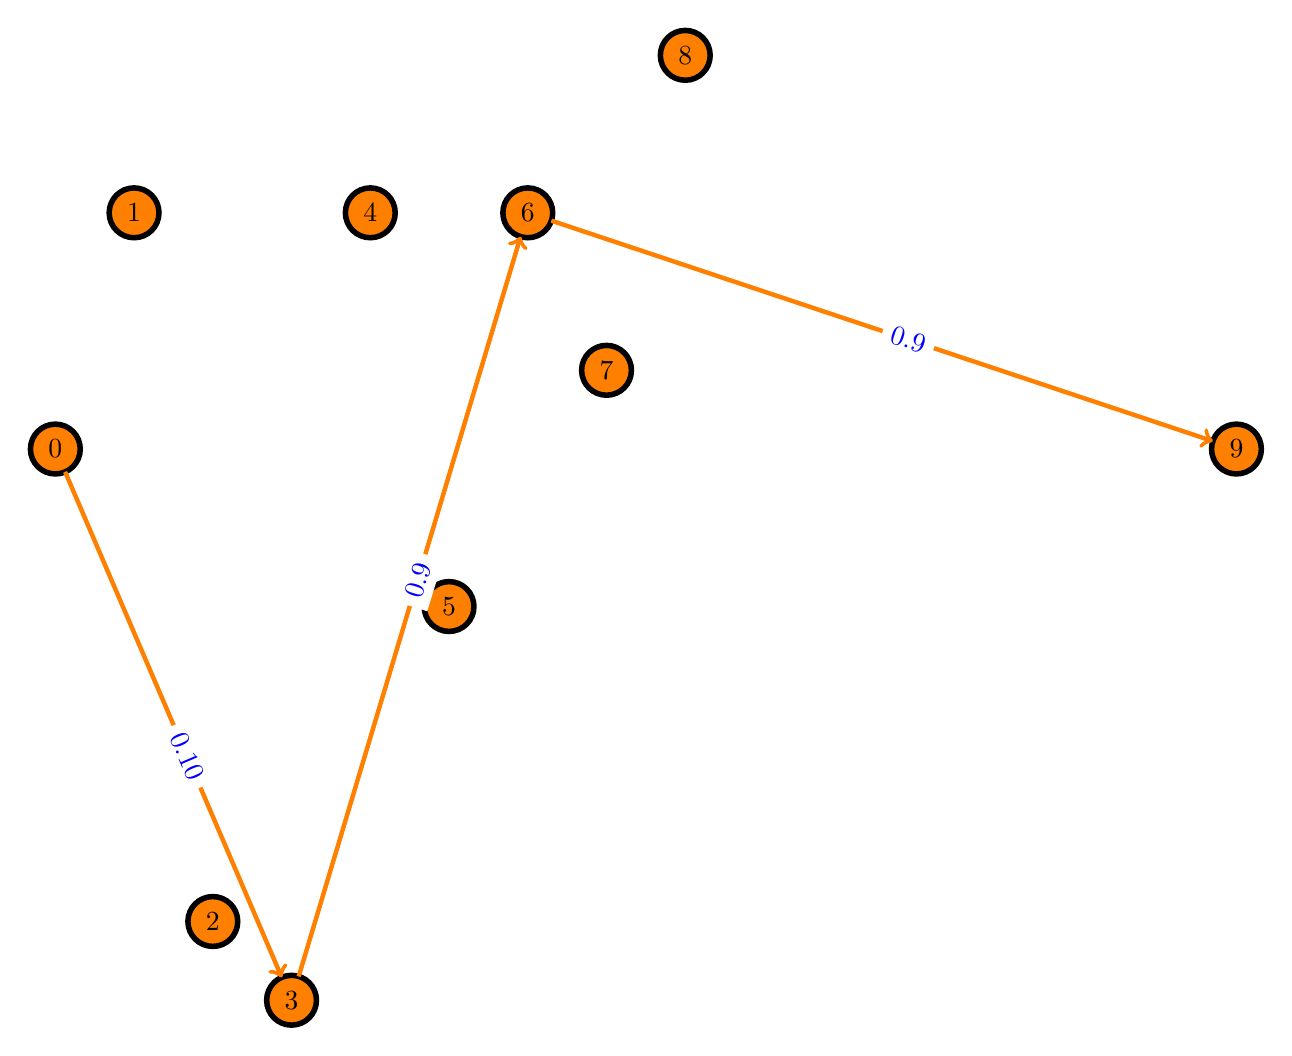
\begin{tikzpicture}
\SetVertexNormal[Shape      = circle,
FillColor  = orange,
LineWidth  = 2pt]
\SetUpEdge[lw         = 0.5pt,
color      = black,
labelcolor = white,
labeltext  = red,
labelstyle = {sloped,text=blue}]
\tikzstyle{TempStyle}=[double = orange]
\Vertex[x=-10, y=8]{0}
\Vertex[x=-9, y=11]{1}
\Vertex[x=-8, y=2]{2}
\Vertex[x=-7, y=1]{3}
\Vertex[x=-6, y=11]{4}
\Vertex[x=-5, y=6]{5}
\Vertex[x=-4, y=11]{6}
\Vertex[x=-3, y=9]{7}
\Vertex[x=-2, y=13]{8}
\Vertex[x=5, y=8]{9}
\tikzset{EdgeStyle/.style={->,TempStyle,relative=false,right=60,color=orange}}
\Edge[label=$0.10$](0)(3)
\tikzset{EdgeStyle/.style={->,TempStyle,relative=false,right=60,color=orange}}
\Edge[label=$0.9$](3)(6)
\tikzset{EdgeStyle/.style={->,TempStyle,relative=false,right=60,color=orange}}
\Edge[label=$0.9$](6)(9)
\end{tikzpicture}\\
\begin{center}\begin{tabular}{l c}\\
\textcolor{orange}{\LARGE$\rightarrow$} & Chemin \\
 \textcolor{red}{\LARGE$\rightarrow$} & Créations arcs\\
 \textcolor{green}{\LARGE$\rightarrow$} & Modification flot\\
\end{tabular}
\end{center}
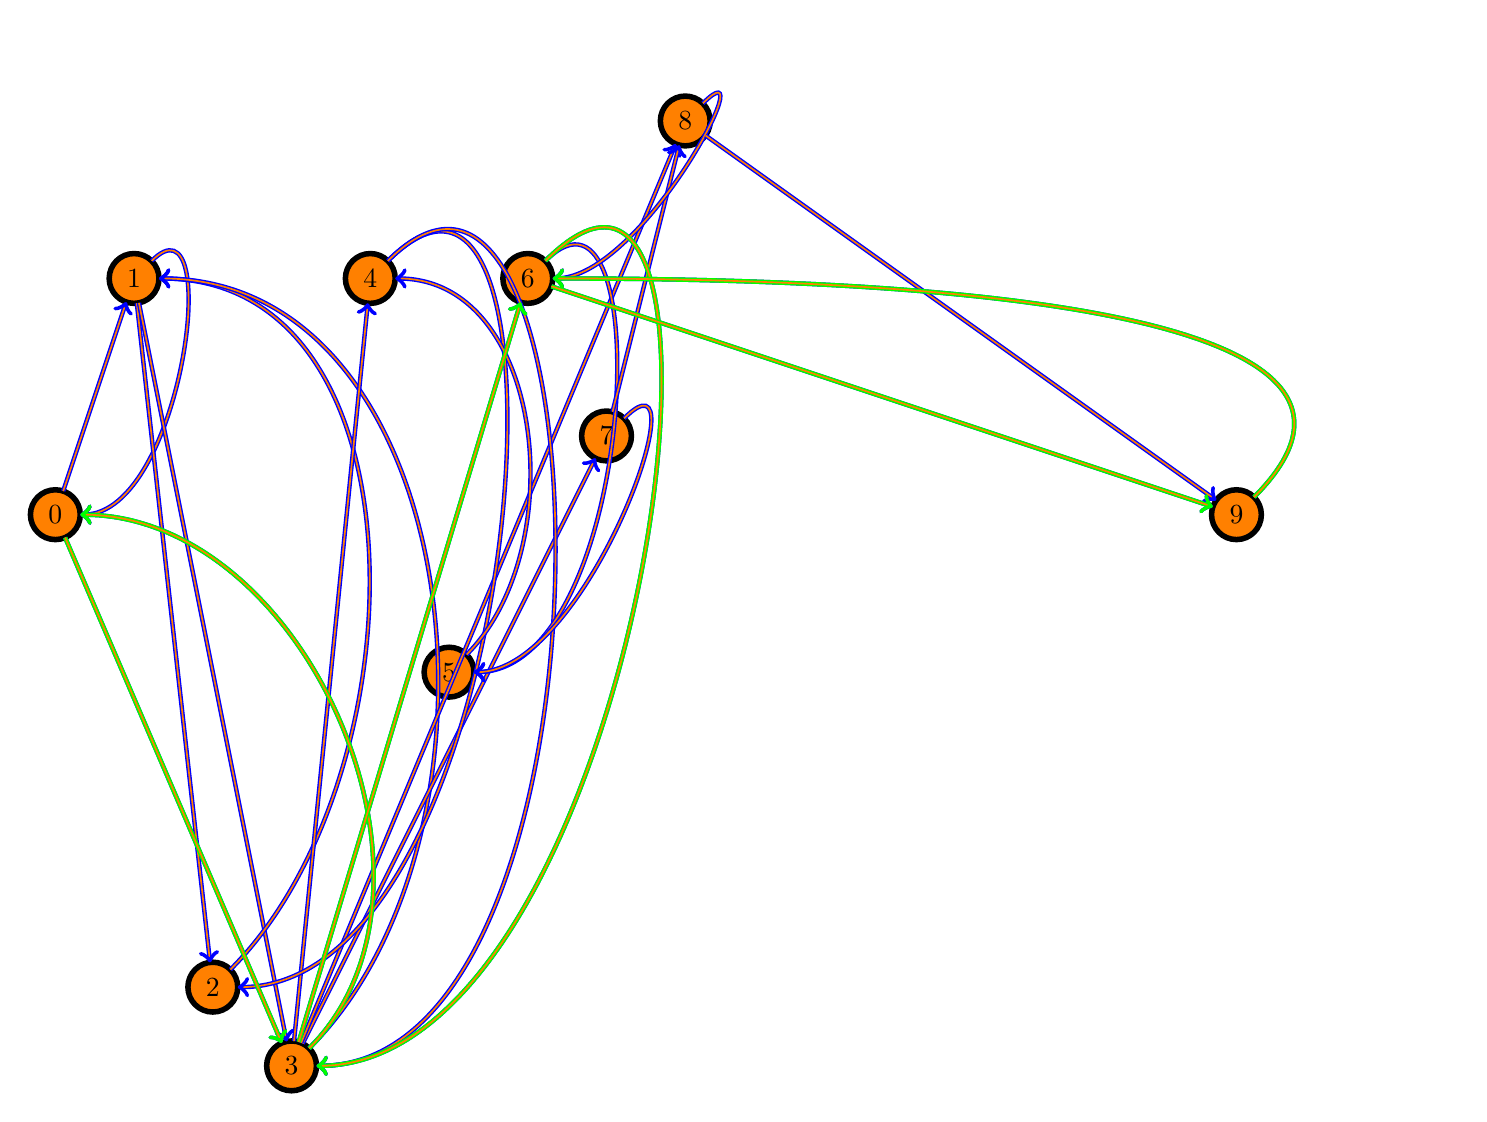
\begin{tikzpicture}
\SetVertexNormal[Shape      = circle,
FillColor  = orange,
LineWidth  = 2pt]
\SetUpEdge[lw         = 0.5pt,
color      = black,
labelcolor = white,
labeltext  = red,
labelstyle = {sloped,text=blue}]
\tikzstyle{TempStyle}=[double = orange]
\Vertex[x=-10, y=8]{0}
\Vertex[x=-9, y=11]{1}
\Vertex[x=-8, y=2]{2}
\Vertex[x=-7, y=1]{3}
\Vertex[x=-6, y=11]{4}
\Vertex[x=-5, y=6]{5}
\Vertex[x=-4, y=11]{6}
\Vertex[x=-3, y=9]{7}
\Vertex[x=-2, y=13]{8}
\Vertex[x=5, y=8]{9}
\tikzset{EdgeStyle/.style={->,TempStyle,relative=false,right=60,color=blue}}
\Edge(0)(1)
\tikzset{EdgeStyle/.style={->,TempStyle,relative=false,right=60,color=blue}}
\Edge(0)(3)
\tikzset{EdgeStyle/.style={->,TempStyle,relative=false,left=60,color=blue,in=0,draw}}
\Edge(1)(0)
\tikzset{EdgeStyle/.style={->,TempStyle,relative=false,right=60,color=blue}}
\Edge(1)(2)
\tikzset{EdgeStyle/.style={->,TempStyle,relative=false,right=60,color=blue}}
\Edge(1)(3)
\tikzset{EdgeStyle/.style={->,TempStyle,relative=false,left=60,color=blue,in=0,draw}}
\Edge(2)(1)
\tikzset{EdgeStyle/.style={->,TempStyle,relative=false,left=60,color=blue,in=0,draw}}
\Edge(3)(0)
\tikzset{EdgeStyle/.style={->,TempStyle,relative=false,left=60,color=blue,in=0,draw}}
\Edge(3)(1)
\tikzset{EdgeStyle/.style={->,TempStyle,relative=false,right=60,color=blue}}
\Edge(3)(4)
\tikzset{EdgeStyle/.style={->,TempStyle,relative=false,right=60,color=blue}}
\Edge(3)(6)
\tikzset{EdgeStyle/.style={->,TempStyle,relative=false,right=60,color=blue}}
\Edge(3)(7)
\tikzset{EdgeStyle/.style={->,TempStyle,relative=false,right=60,color=blue}}
\Edge(3)(8)
\tikzset{EdgeStyle/.style={->,TempStyle,relative=false,left=60,color=blue,in=0,draw}}
\Edge(4)(2)
\tikzset{EdgeStyle/.style={->,TempStyle,relative=false,left=60,color=blue,in=0,draw}}
\Edge(4)(3)
\tikzset{EdgeStyle/.style={->,TempStyle,relative=false,left=60,color=blue,in=0,draw}}
\Edge(5)(4)
\tikzset{EdgeStyle/.style={->,TempStyle,relative=false,left=60,color=blue,in=0,draw}}
\Edge(6)(3)
\tikzset{EdgeStyle/.style={->,TempStyle,relative=false,left=60,color=blue,in=0,draw}}
\Edge(6)(5)
\tikzset{EdgeStyle/.style={->,TempStyle,relative=false,right=60,color=blue}}
\Edge(6)(9)
\tikzset{EdgeStyle/.style={->,TempStyle,relative=false,left=60,color=blue,in=0,draw}}
\Edge(7)(5)
\tikzset{EdgeStyle/.style={->,TempStyle,relative=false,right=60,color=blue}}
\Edge(7)(8)
\tikzset{EdgeStyle/.style={->,TempStyle,relative=false,left=60,color=blue,in=0,draw}}
\Edge(8)(6)
\tikzset{EdgeStyle/.style={->,TempStyle,relative=false,right=60,color=blue}}
\Edge(8)(9)
\tikzset{EdgeStyle/.style={->,TempStyle,relative=false,left=60,color=blue,in=0,draw}}
\Edge(9)(6)
\tikzset{EdgeStyle/.style={->,TempStyle,relative=false,right=60,color=green}}
\Edge(0)(3)
\tikzset{EdgeStyle/.style={->,TempStyle,relative=false,right=60,in=0,color=green}}
\Edge(3)(0)
\tikzset{EdgeStyle/.style={->,TempStyle,relative=false,right=60,color=green}}
\Edge(3)(6)
\tikzset{EdgeStyle/.style={->,TempStyle,relative=false,right=60,in=0,color=green}}
\Edge(6)(3)
\tikzset{EdgeStyle/.style={->,TempStyle,relative=false,right=60,color=green}}
\Edge(6)(9)
\tikzset{EdgeStyle/.style={->,TempStyle,relative=false,right=60,in=0,color=green}}
\Edge(9)(6)
\end{tikzpicture}\\
\begin{center}\begin{tabular}{l c}\\
\textcolor{orange}{\LARGE$\rightarrow$} & Chemin \\
 \textcolor{red}{\LARGE$\rightarrow$} & Créations arcs\\
 \textcolor{green}{\LARGE$\rightarrow$} & Modification flot\\
\end{tabular}
\end{center}
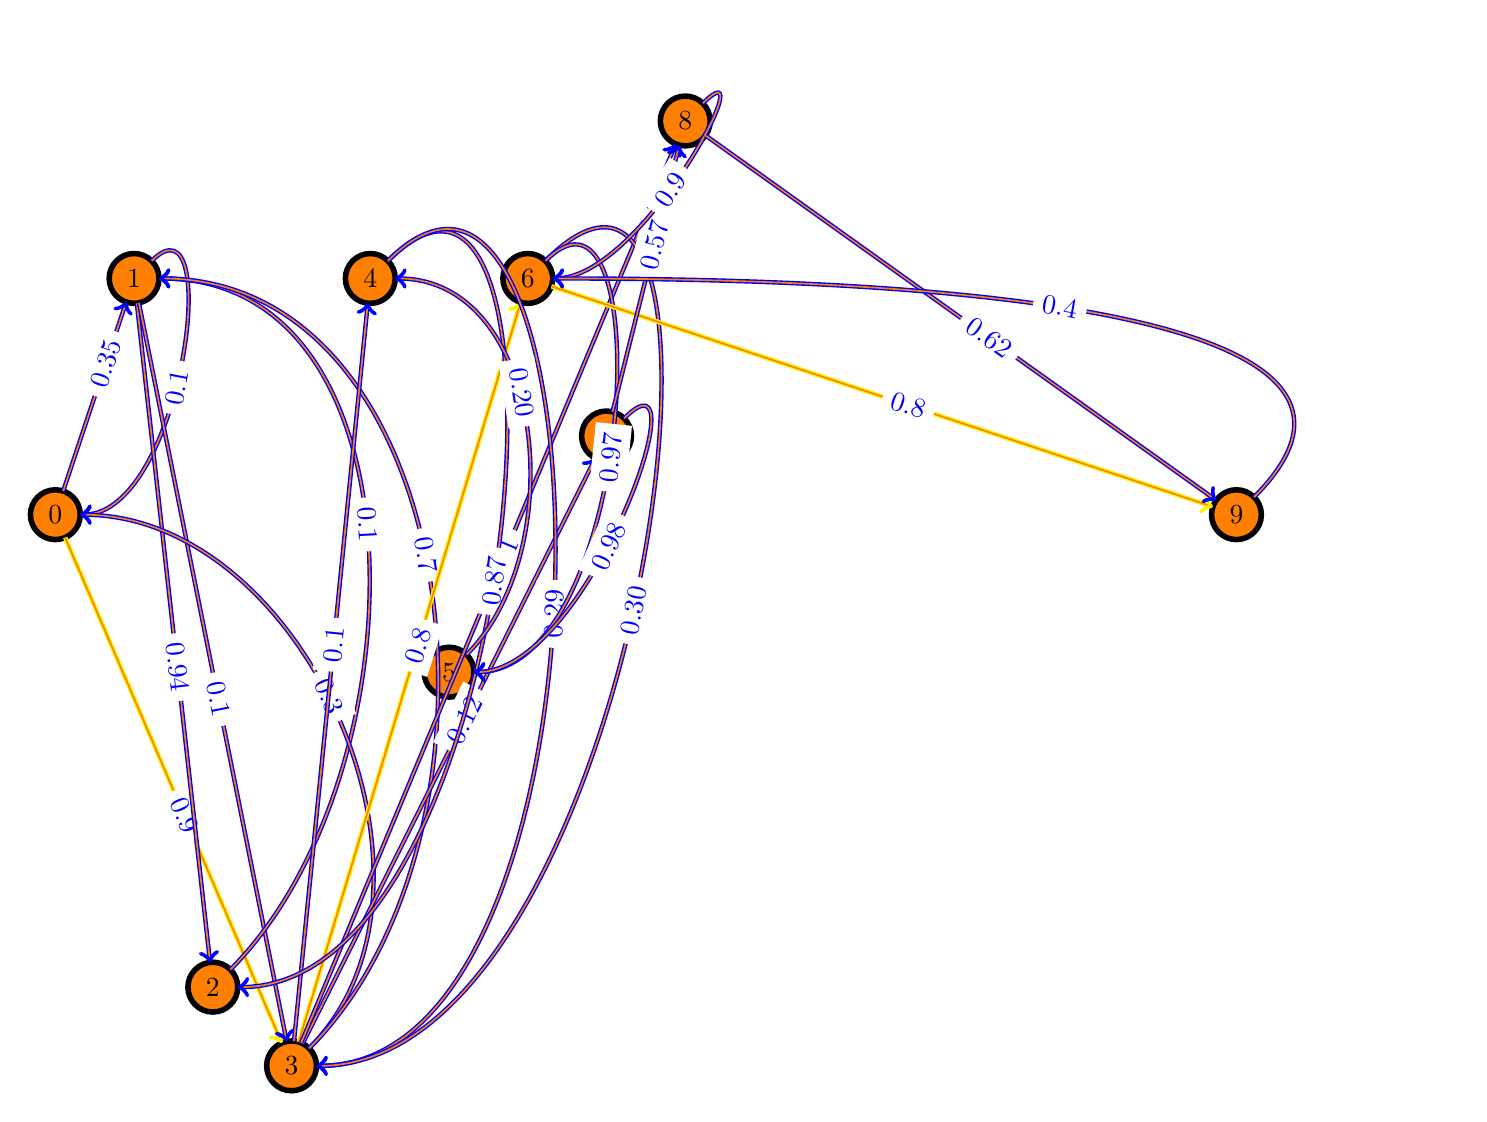
\begin{tikzpicture}
\SetVertexNormal[Shape      = circle,
FillColor  = orange,
LineWidth  = 2pt]
\SetUpEdge[lw         = 0.5pt,
color      = black,
labelcolor = white,
labeltext  = red,
labelstyle = {sloped,text=blue}]
\tikzstyle{TempStyle}=[double = orange]
\Vertex[x=-10, y=8]{0}
\Vertex[x=-9, y=11]{1}
\Vertex[x=-8, y=2]{2}
\Vertex[x=-7, y=1]{3}
\Vertex[x=-6, y=11]{4}
\Vertex[x=-5, y=6]{5}
\Vertex[x=-4, y=11]{6}
\Vertex[x=-3, y=9]{7}
\Vertex[x=-2, y=13]{8}
\Vertex[x=5, y=8]{9}
\tikzset{EdgeStyle/.style={->,TempStyle,relative=false,right=60,color=blue}}
\Edge[label=$0.35$](0)(1)
\tikzset{EdgeStyle/.style={->,TempStyle,relative=false,right=60,color=yellow}}
\Edge[label=$0.9$](0)(3)
\tikzset{EdgeStyle/.style={->,TempStyle,relative=false,left=60,color=blue,in=0,draw}}
\Edge[label=$0.1$](1)(0)
\tikzset{EdgeStyle/.style={->,TempStyle,relative=false,right=60,color=blue}}
\Edge[label=$0.94$](1)(2)
\tikzset{EdgeStyle/.style={->,TempStyle,relative=false,right=60,color=blue}}
\Edge[label=$0.1$](1)(3)
\tikzset{EdgeStyle/.style={->,TempStyle,relative=false,left=60,color=blue,in=0,draw}}
\Edge[label=$0.1$](2)(1)
\tikzset{EdgeStyle/.style={->,TempStyle,relative=false,left=60,color=blue,in=0,draw}}
\Edge[label=$0.3$](3)(0)
\tikzset{EdgeStyle/.style={->,TempStyle,relative=false,left=60,color=blue,in=0,draw}}
\Edge[label=$0.7$](3)(1)
\tikzset{EdgeStyle/.style={->,TempStyle,relative=false,right=60,color=blue}}
\Edge[label=$0.1$](3)(4)
\tikzset{EdgeStyle/.style={->,TempStyle,relative=false,right=60,color=yellow}}
\Edge[label=$0.8$](3)(6)
\tikzset{EdgeStyle/.style={->,TempStyle,relative=false,right=60,color=blue}}
\Edge[label=$0.12$](3)(7)
\tikzset{EdgeStyle/.style={->,TempStyle,relative=false,right=60,color=blue}}
\Edge[label=$0.61$](3)(8)
\tikzset{EdgeStyle/.style={->,TempStyle,relative=false,left=60,color=blue,in=0,draw}}
\Edge[label=$0.87$](4)(2)
\tikzset{EdgeStyle/.style={->,TempStyle,relative=false,left=60,color=blue,in=0,draw}}
\Edge[label=$0.29$](4)(3)
\tikzset{EdgeStyle/.style={->,TempStyle,relative=false,left=60,color=blue,in=0,draw}}
\Edge[label=$0.20$](5)(4)
\tikzset{EdgeStyle/.style={->,TempStyle,relative=false,left=60,color=blue,in=0,draw}}
\Edge[label=$0.30$](6)(3)
\tikzset{EdgeStyle/.style={->,TempStyle,relative=false,left=60,color=blue,in=0,draw}}
\Edge[label=$0.97$](6)(5)
\tikzset{EdgeStyle/.style={->,TempStyle,relative=false,right=60,color=yellow}}
\Edge[label=$0.8$](6)(9)
\tikzset{EdgeStyle/.style={->,TempStyle,relative=false,left=60,color=blue,in=0,draw}}
\Edge[label=$0.98$](7)(5)
\tikzset{EdgeStyle/.style={->,TempStyle,relative=false,right=60,color=blue}}
\Edge[label=$0.57$](7)(8)
\tikzset{EdgeStyle/.style={->,TempStyle,relative=false,left=60,color=blue,in=0,draw}}
\Edge[label=$0.9$](8)(6)
\tikzset{EdgeStyle/.style={->,TempStyle,relative=false,right=60,color=blue}}
\Edge[label=$0.62$](8)(9)
\tikzset{EdgeStyle/.style={->,TempStyle,relative=false,left=60,color=blue,in=0,draw}}
\Edge[label=$0.4$](9)(6)
\end{tikzpicture}\\
\begin{center}\begin{tabular}{l c}\\
\textcolor{orange}{\LARGE$\rightarrow$} & Chemin \\
 \textcolor{red}{\LARGE$\rightarrow$} & Créations arcs\\
 \textcolor{green}{\LARGE$\rightarrow$} & Modification flot\\
\end{tabular}
\end{center}
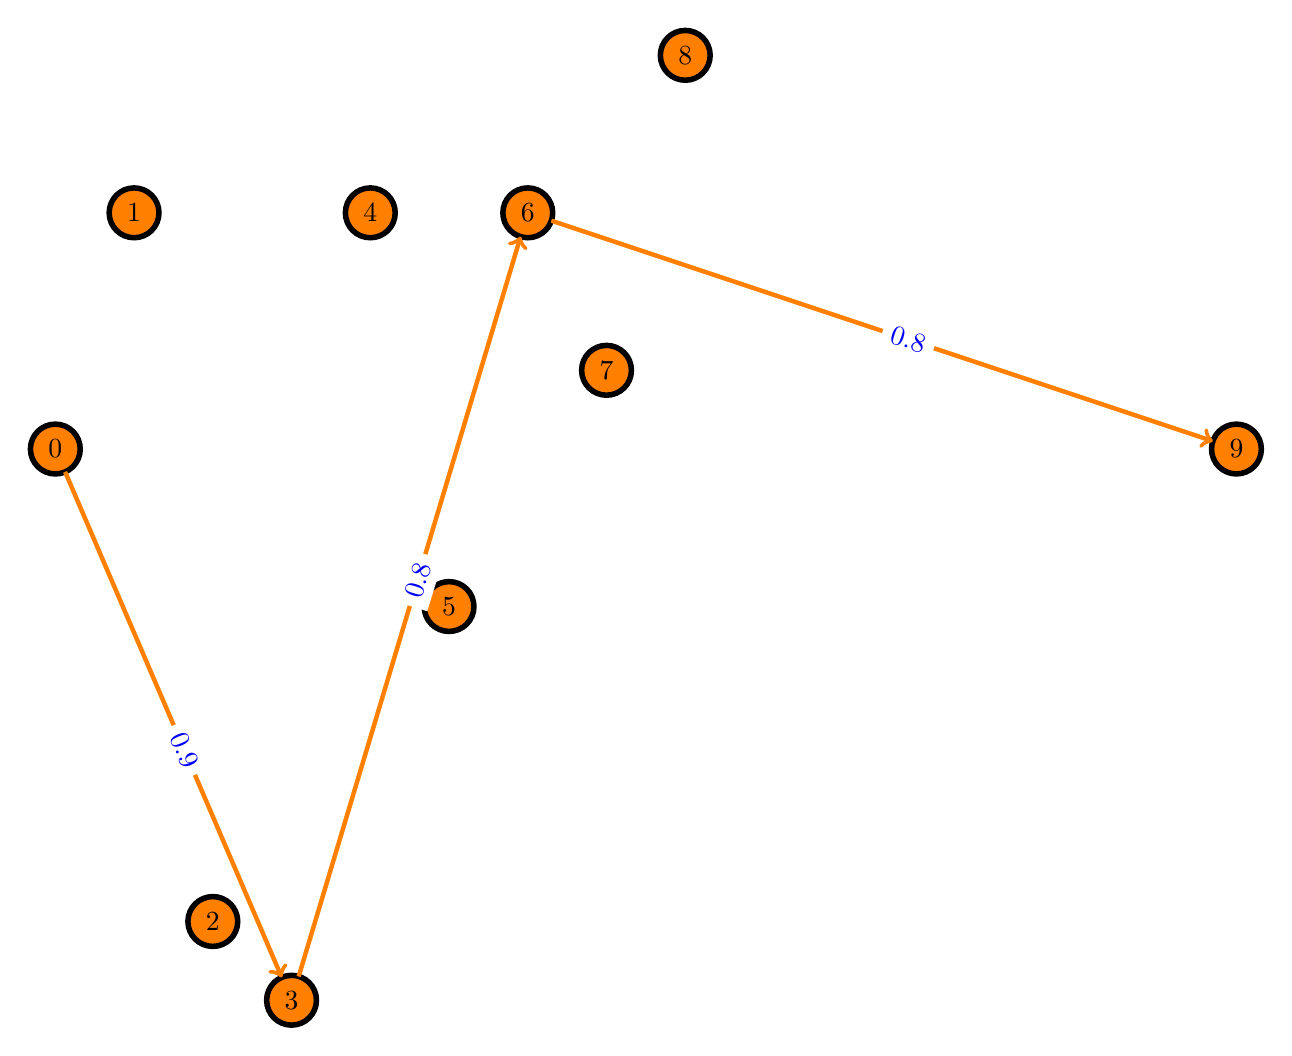
\begin{tikzpicture}
\SetVertexNormal[Shape      = circle,
FillColor  = orange,
LineWidth  = 2pt]
\SetUpEdge[lw         = 0.5pt,
color      = black,
labelcolor = white,
labeltext  = red,
labelstyle = {sloped,text=blue}]
\tikzstyle{TempStyle}=[double = orange]
\Vertex[x=-10, y=8]{0}
\Vertex[x=-9, y=11]{1}
\Vertex[x=-8, y=2]{2}
\Vertex[x=-7, y=1]{3}
\Vertex[x=-6, y=11]{4}
\Vertex[x=-5, y=6]{5}
\Vertex[x=-4, y=11]{6}
\Vertex[x=-3, y=9]{7}
\Vertex[x=-2, y=13]{8}
\Vertex[x=5, y=8]{9}
\tikzset{EdgeStyle/.style={->,TempStyle,relative=false,right=60,color=orange}}
\Edge[label=$0.9$](0)(3)
\tikzset{EdgeStyle/.style={->,TempStyle,relative=false,right=60,color=orange}}
\Edge[label=$0.8$](3)(6)
\tikzset{EdgeStyle/.style={->,TempStyle,relative=false,right=60,color=orange}}
\Edge[label=$0.8$](6)(9)
\end{tikzpicture}\\
\begin{center}\begin{tabular}{l c}\\
\textcolor{orange}{\LARGE$\rightarrow$} & Chemin \\
 \textcolor{red}{\LARGE$\rightarrow$} & Créations arcs\\
 \textcolor{green}{\LARGE$\rightarrow$} & Modification flot\\
\end{tabular}
\end{center}
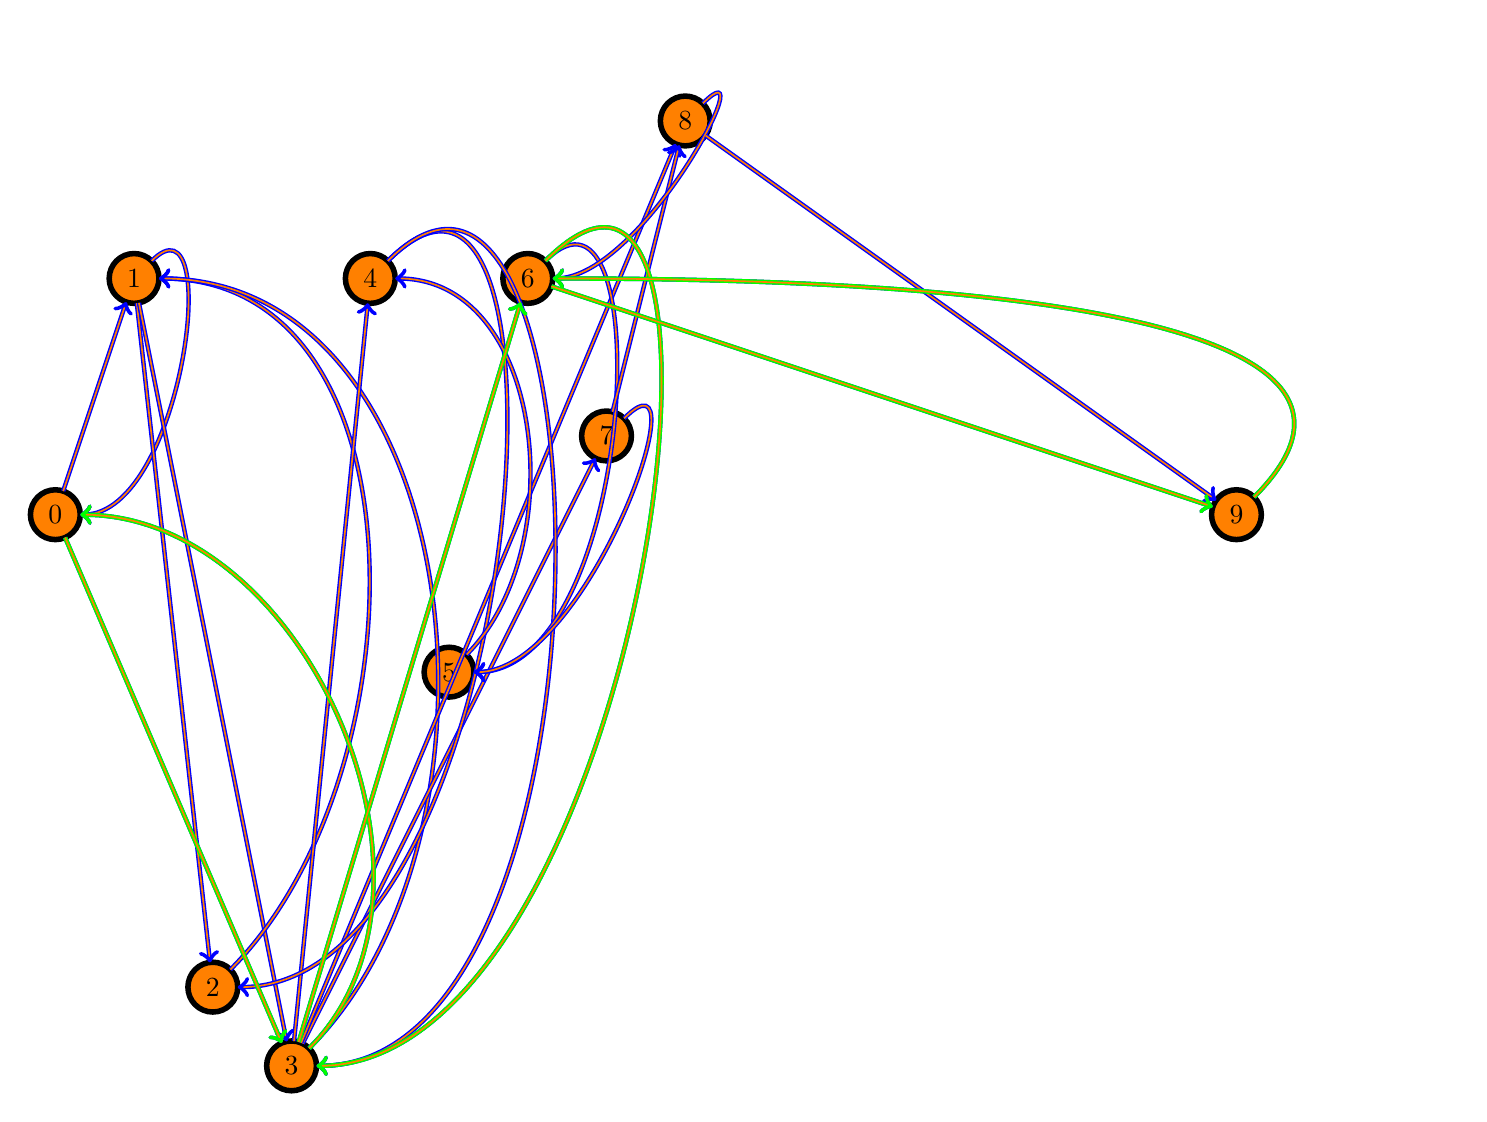
\begin{tikzpicture}
\SetVertexNormal[Shape      = circle,
FillColor  = orange,
LineWidth  = 2pt]
\SetUpEdge[lw         = 0.5pt,
color      = black,
labelcolor = white,
labeltext  = red,
labelstyle = {sloped,text=blue}]
\tikzstyle{TempStyle}=[double = orange]
\Vertex[x=-10, y=8]{0}
\Vertex[x=-9, y=11]{1}
\Vertex[x=-8, y=2]{2}
\Vertex[x=-7, y=1]{3}
\Vertex[x=-6, y=11]{4}
\Vertex[x=-5, y=6]{5}
\Vertex[x=-4, y=11]{6}
\Vertex[x=-3, y=9]{7}
\Vertex[x=-2, y=13]{8}
\Vertex[x=5, y=8]{9}
\tikzset{EdgeStyle/.style={->,TempStyle,relative=false,right=60,color=blue}}
\Edge(0)(1)
\tikzset{EdgeStyle/.style={->,TempStyle,relative=false,right=60,color=blue}}
\Edge(0)(3)
\tikzset{EdgeStyle/.style={->,TempStyle,relative=false,left=60,color=blue,in=0,draw}}
\Edge(1)(0)
\tikzset{EdgeStyle/.style={->,TempStyle,relative=false,right=60,color=blue}}
\Edge(1)(2)
\tikzset{EdgeStyle/.style={->,TempStyle,relative=false,right=60,color=blue}}
\Edge(1)(3)
\tikzset{EdgeStyle/.style={->,TempStyle,relative=false,left=60,color=blue,in=0,draw}}
\Edge(2)(1)
\tikzset{EdgeStyle/.style={->,TempStyle,relative=false,left=60,color=blue,in=0,draw}}
\Edge(3)(0)
\tikzset{EdgeStyle/.style={->,TempStyle,relative=false,left=60,color=blue,in=0,draw}}
\Edge(3)(1)
\tikzset{EdgeStyle/.style={->,TempStyle,relative=false,right=60,color=blue}}
\Edge(3)(4)
\tikzset{EdgeStyle/.style={->,TempStyle,relative=false,right=60,color=blue}}
\Edge(3)(6)
\tikzset{EdgeStyle/.style={->,TempStyle,relative=false,right=60,color=blue}}
\Edge(3)(7)
\tikzset{EdgeStyle/.style={->,TempStyle,relative=false,right=60,color=blue}}
\Edge(3)(8)
\tikzset{EdgeStyle/.style={->,TempStyle,relative=false,left=60,color=blue,in=0,draw}}
\Edge(4)(2)
\tikzset{EdgeStyle/.style={->,TempStyle,relative=false,left=60,color=blue,in=0,draw}}
\Edge(4)(3)
\tikzset{EdgeStyle/.style={->,TempStyle,relative=false,left=60,color=blue,in=0,draw}}
\Edge(5)(4)
\tikzset{EdgeStyle/.style={->,TempStyle,relative=false,left=60,color=blue,in=0,draw}}
\Edge(6)(3)
\tikzset{EdgeStyle/.style={->,TempStyle,relative=false,left=60,color=blue,in=0,draw}}
\Edge(6)(5)
\tikzset{EdgeStyle/.style={->,TempStyle,relative=false,right=60,color=blue}}
\Edge(6)(9)
\tikzset{EdgeStyle/.style={->,TempStyle,relative=false,left=60,color=blue,in=0,draw}}
\Edge(7)(5)
\tikzset{EdgeStyle/.style={->,TempStyle,relative=false,right=60,color=blue}}
\Edge(7)(8)
\tikzset{EdgeStyle/.style={->,TempStyle,relative=false,left=60,color=blue,in=0,draw}}
\Edge(8)(6)
\tikzset{EdgeStyle/.style={->,TempStyle,relative=false,right=60,color=blue}}
\Edge(8)(9)
\tikzset{EdgeStyle/.style={->,TempStyle,relative=false,left=60,color=blue,in=0,draw}}
\Edge(9)(6)
\tikzset{EdgeStyle/.style={->,TempStyle,relative=false,right=60,color=green}}
\Edge(0)(3)
\tikzset{EdgeStyle/.style={->,TempStyle,relative=false,right=60,in=0,color=green}}
\Edge(3)(0)
\tikzset{EdgeStyle/.style={->,TempStyle,relative=false,right=60,color=green}}
\Edge(3)(6)
\tikzset{EdgeStyle/.style={->,TempStyle,relative=false,right=60,in=0,color=green}}
\Edge(6)(3)
\tikzset{EdgeStyle/.style={->,TempStyle,relative=false,right=60,color=green}}
\Edge(6)(9)
\tikzset{EdgeStyle/.style={->,TempStyle,relative=false,right=60,in=0,color=green}}
\Edge(9)(6)
\end{tikzpicture}\\
\begin{center}\begin{tabular}{l c}\\
\textcolor{orange}{\LARGE$\rightarrow$} & Chemin \\
 \textcolor{red}{\LARGE$\rightarrow$} & Créations arcs\\
 \textcolor{green}{\LARGE$\rightarrow$} & Modification flot\\
\end{tabular}
\end{center}
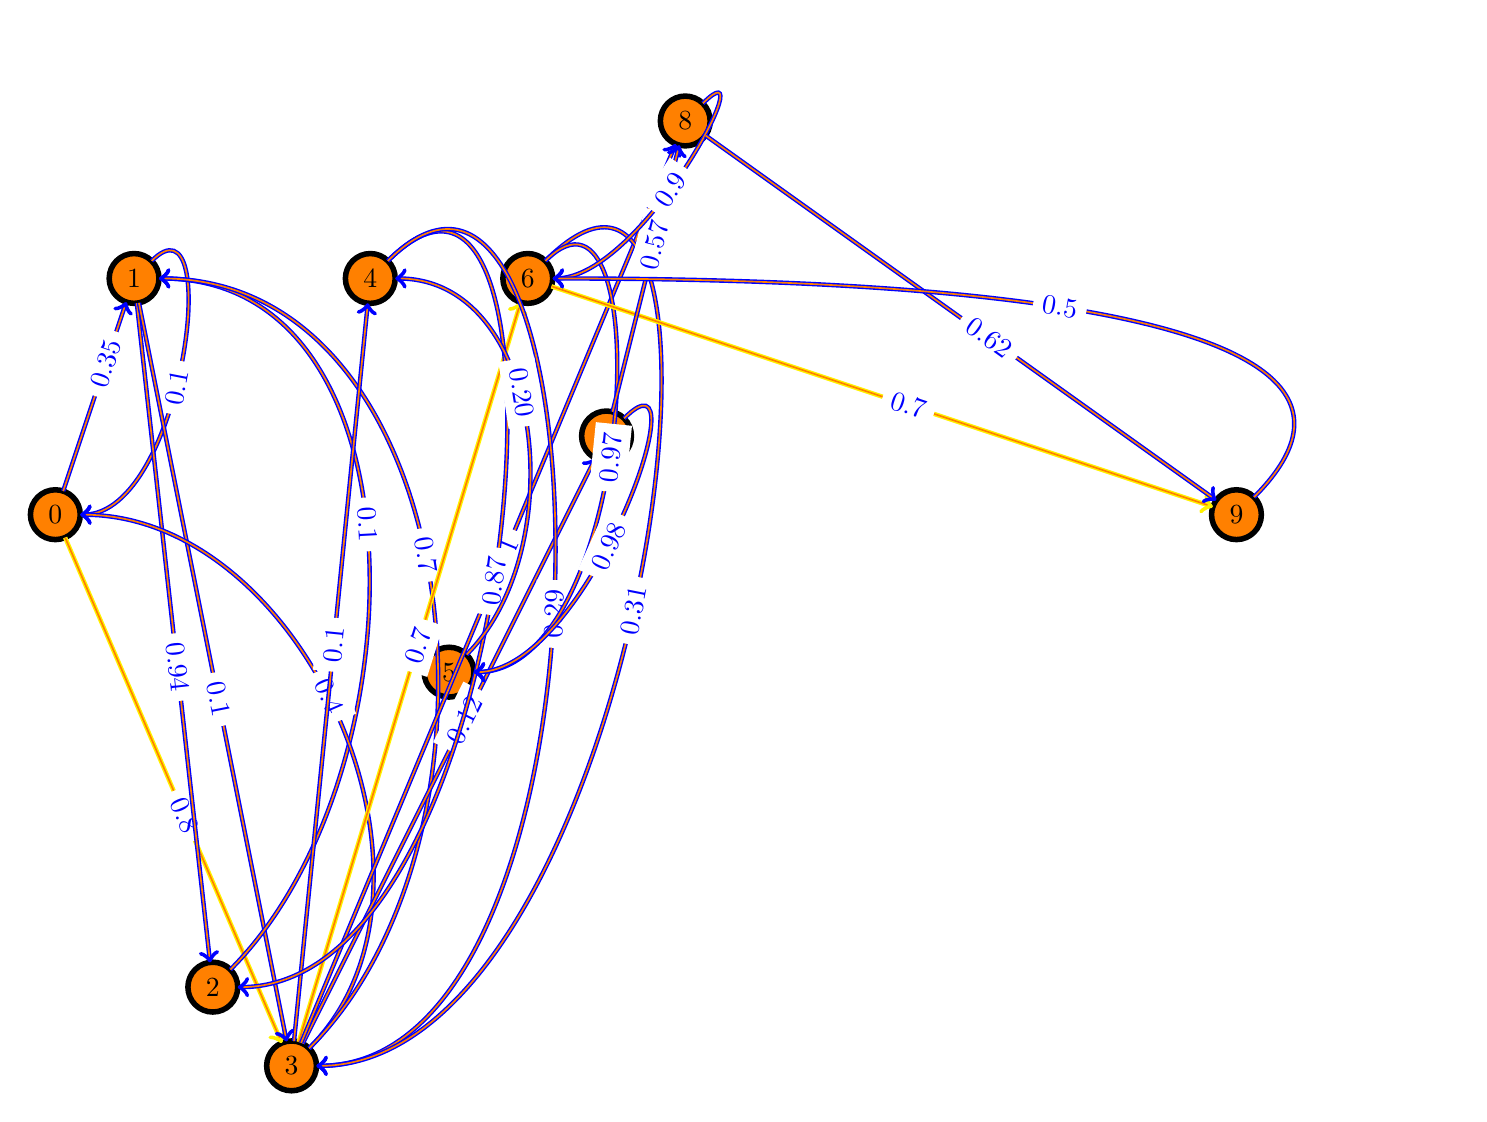
\begin{tikzpicture}
\SetVertexNormal[Shape      = circle,
FillColor  = orange,
LineWidth  = 2pt]
\SetUpEdge[lw         = 0.5pt,
color      = black,
labelcolor = white,
labeltext  = red,
labelstyle = {sloped,text=blue}]
\tikzstyle{TempStyle}=[double = orange]
\Vertex[x=-10, y=8]{0}
\Vertex[x=-9, y=11]{1}
\Vertex[x=-8, y=2]{2}
\Vertex[x=-7, y=1]{3}
\Vertex[x=-6, y=11]{4}
\Vertex[x=-5, y=6]{5}
\Vertex[x=-4, y=11]{6}
\Vertex[x=-3, y=9]{7}
\Vertex[x=-2, y=13]{8}
\Vertex[x=5, y=8]{9}
\tikzset{EdgeStyle/.style={->,TempStyle,relative=false,right=60,color=blue}}
\Edge[label=$0.35$](0)(1)
\tikzset{EdgeStyle/.style={->,TempStyle,relative=false,right=60,color=yellow}}
\Edge[label=$0.8$](0)(3)
\tikzset{EdgeStyle/.style={->,TempStyle,relative=false,left=60,color=blue,in=0,draw}}
\Edge[label=$0.1$](1)(0)
\tikzset{EdgeStyle/.style={->,TempStyle,relative=false,right=60,color=blue}}
\Edge[label=$0.94$](1)(2)
\tikzset{EdgeStyle/.style={->,TempStyle,relative=false,right=60,color=blue}}
\Edge[label=$0.1$](1)(3)
\tikzset{EdgeStyle/.style={->,TempStyle,relative=false,left=60,color=blue,in=0,draw}}
\Edge[label=$0.1$](2)(1)
\tikzset{EdgeStyle/.style={->,TempStyle,relative=false,left=60,color=blue,in=0,draw}}
\Edge[label=$0.4$](3)(0)
\tikzset{EdgeStyle/.style={->,TempStyle,relative=false,left=60,color=blue,in=0,draw}}
\Edge[label=$0.7$](3)(1)
\tikzset{EdgeStyle/.style={->,TempStyle,relative=false,right=60,color=blue}}
\Edge[label=$0.1$](3)(4)
\tikzset{EdgeStyle/.style={->,TempStyle,relative=false,right=60,color=yellow}}
\Edge[label=$0.7$](3)(6)
\tikzset{EdgeStyle/.style={->,TempStyle,relative=false,right=60,color=blue}}
\Edge[label=$0.12$](3)(7)
\tikzset{EdgeStyle/.style={->,TempStyle,relative=false,right=60,color=blue}}
\Edge[label=$0.61$](3)(8)
\tikzset{EdgeStyle/.style={->,TempStyle,relative=false,left=60,color=blue,in=0,draw}}
\Edge[label=$0.87$](4)(2)
\tikzset{EdgeStyle/.style={->,TempStyle,relative=false,left=60,color=blue,in=0,draw}}
\Edge[label=$0.29$](4)(3)
\tikzset{EdgeStyle/.style={->,TempStyle,relative=false,left=60,color=blue,in=0,draw}}
\Edge[label=$0.20$](5)(4)
\tikzset{EdgeStyle/.style={->,TempStyle,relative=false,left=60,color=blue,in=0,draw}}
\Edge[label=$0.31$](6)(3)
\tikzset{EdgeStyle/.style={->,TempStyle,relative=false,left=60,color=blue,in=0,draw}}
\Edge[label=$0.97$](6)(5)
\tikzset{EdgeStyle/.style={->,TempStyle,relative=false,right=60,color=yellow}}
\Edge[label=$0.7$](6)(9)
\tikzset{EdgeStyle/.style={->,TempStyle,relative=false,left=60,color=blue,in=0,draw}}
\Edge[label=$0.98$](7)(5)
\tikzset{EdgeStyle/.style={->,TempStyle,relative=false,right=60,color=blue}}
\Edge[label=$0.57$](7)(8)
\tikzset{EdgeStyle/.style={->,TempStyle,relative=false,left=60,color=blue,in=0,draw}}
\Edge[label=$0.9$](8)(6)
\tikzset{EdgeStyle/.style={->,TempStyle,relative=false,right=60,color=blue}}
\Edge[label=$0.62$](8)(9)
\tikzset{EdgeStyle/.style={->,TempStyle,relative=false,left=60,color=blue,in=0,draw}}
\Edge[label=$0.5$](9)(6)
\end{tikzpicture}\\
\begin{center}\begin{tabular}{l c}\\
\textcolor{orange}{\LARGE$\rightarrow$} & Chemin \\
 \textcolor{red}{\LARGE$\rightarrow$} & Créations arcs\\
 \textcolor{green}{\LARGE$\rightarrow$} & Modification flot\\
\end{tabular}
\end{center}
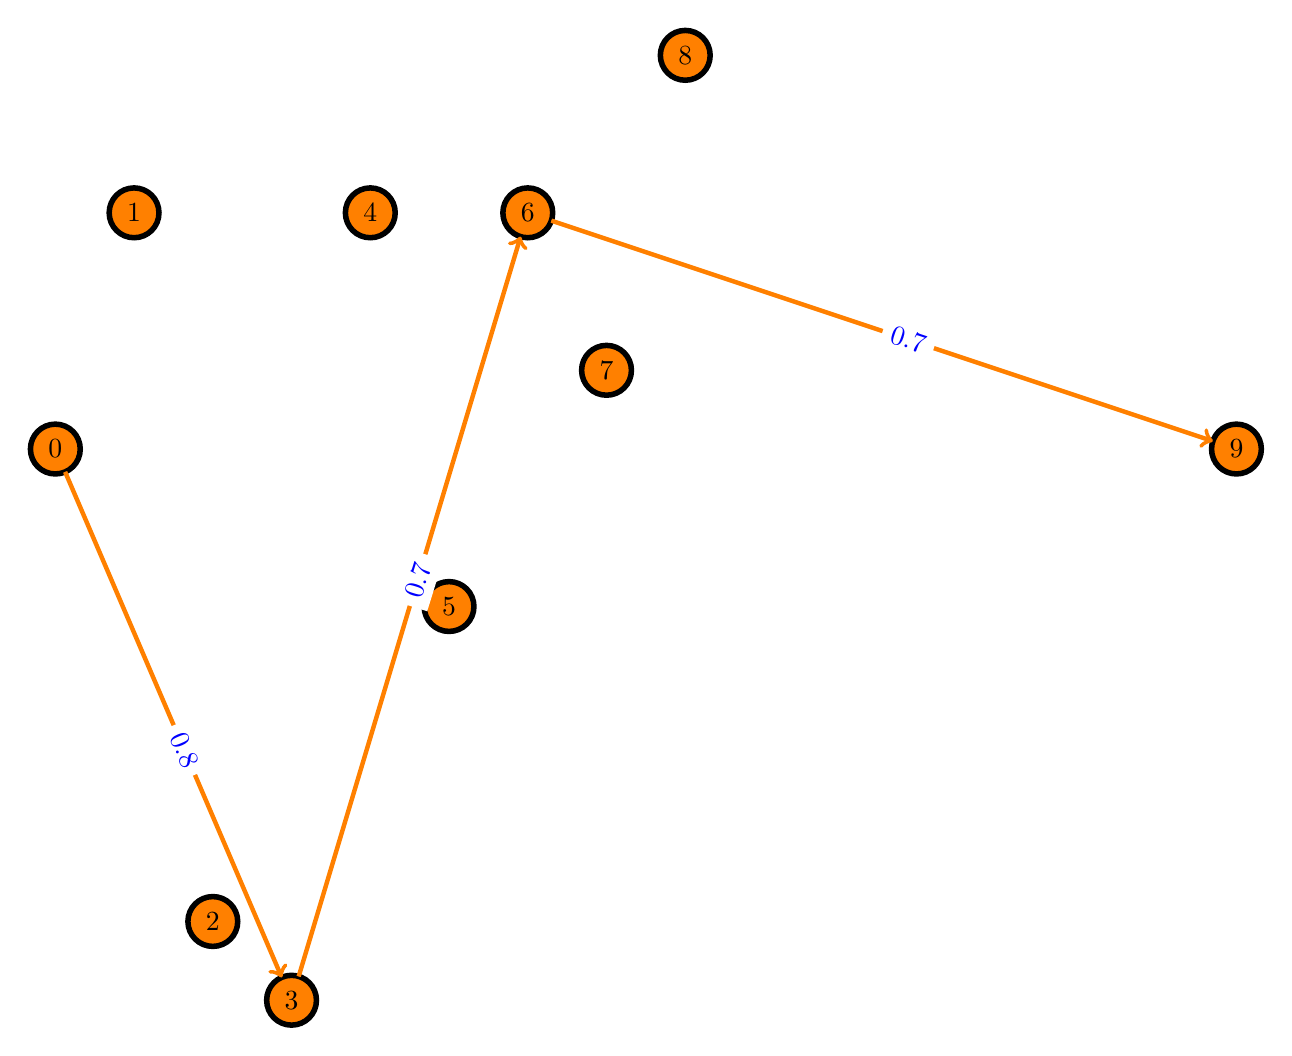
\begin{tikzpicture}
\SetVertexNormal[Shape      = circle,
FillColor  = orange,
LineWidth  = 2pt]
\SetUpEdge[lw         = 0.5pt,
color      = black,
labelcolor = white,
labeltext  = red,
labelstyle = {sloped,text=blue}]
\tikzstyle{TempStyle}=[double = orange]
\Vertex[x=-10, y=8]{0}
\Vertex[x=-9, y=11]{1}
\Vertex[x=-8, y=2]{2}
\Vertex[x=-7, y=1]{3}
\Vertex[x=-6, y=11]{4}
\Vertex[x=-5, y=6]{5}
\Vertex[x=-4, y=11]{6}
\Vertex[x=-3, y=9]{7}
\Vertex[x=-2, y=13]{8}
\Vertex[x=5, y=8]{9}
\tikzset{EdgeStyle/.style={->,TempStyle,relative=false,right=60,color=orange}}
\Edge[label=$0.8$](0)(3)
\tikzset{EdgeStyle/.style={->,TempStyle,relative=false,right=60,color=orange}}
\Edge[label=$0.7$](3)(6)
\tikzset{EdgeStyle/.style={->,TempStyle,relative=false,right=60,color=orange}}
\Edge[label=$0.7$](6)(9)
\end{tikzpicture}\\
\begin{center}\begin{tabular}{l c}\\
\textcolor{orange}{\LARGE$\rightarrow$} & Chemin \\
 \textcolor{red}{\LARGE$\rightarrow$} & Créations arcs\\
 \textcolor{green}{\LARGE$\rightarrow$} & Modification flot\\
\end{tabular}
\end{center}
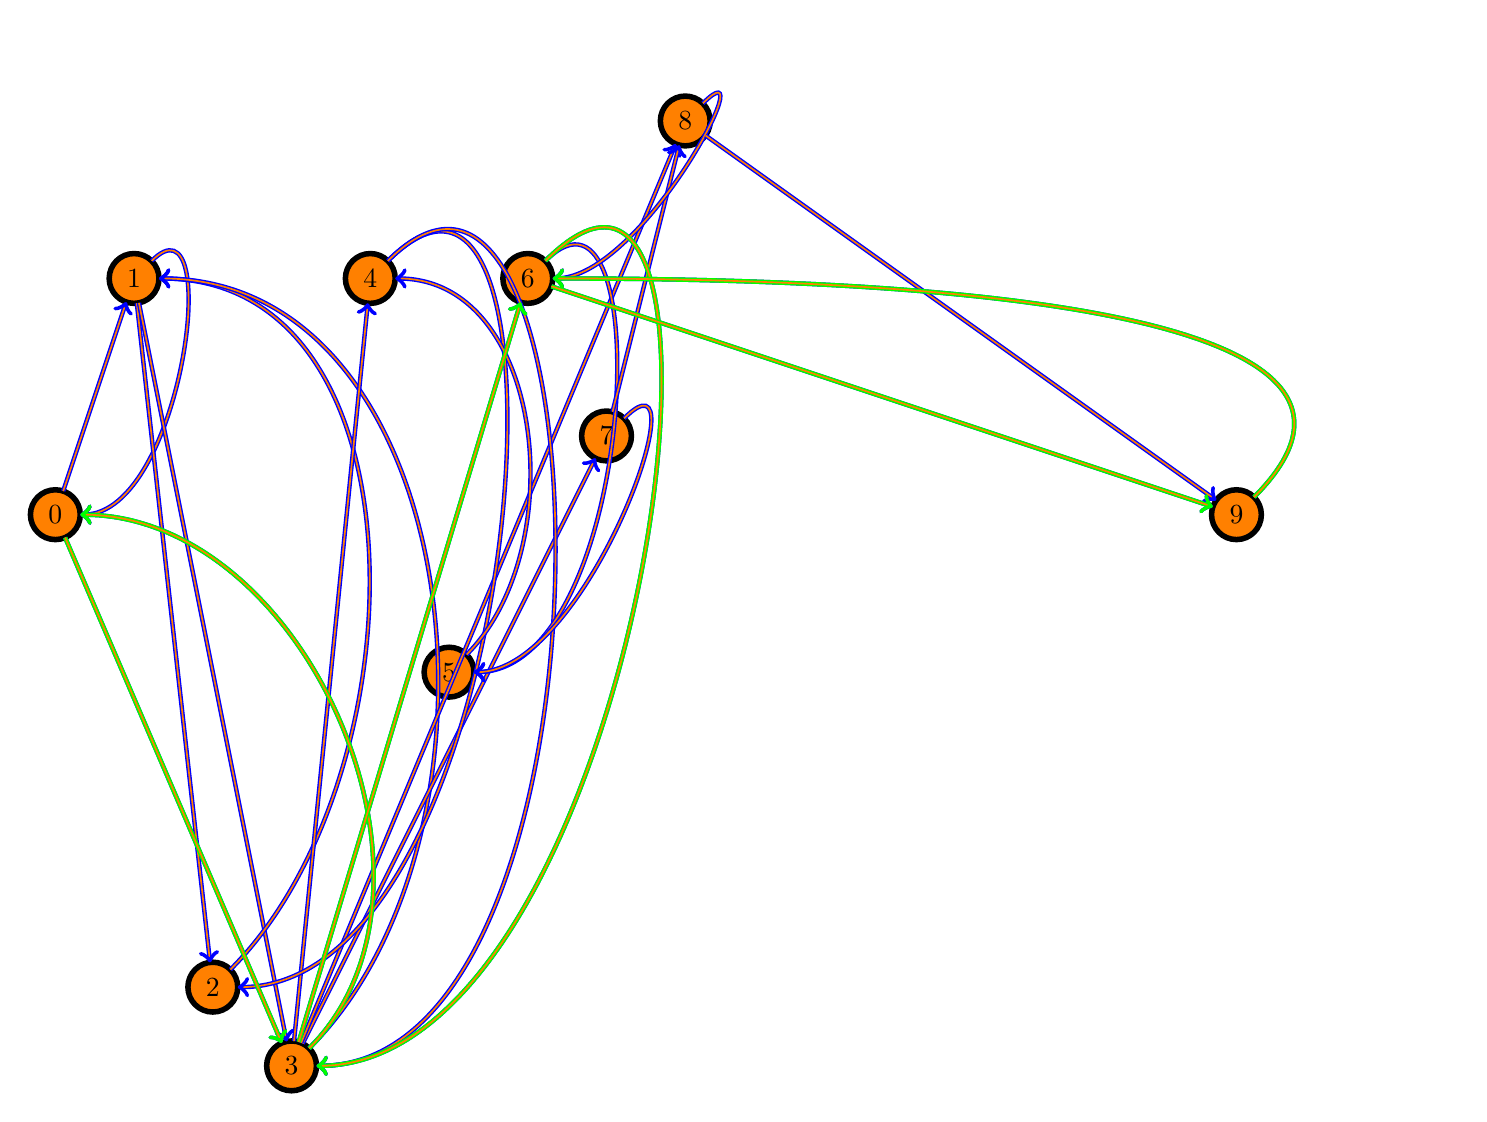
\begin{tikzpicture}
\SetVertexNormal[Shape      = circle,
FillColor  = orange,
LineWidth  = 2pt]
\SetUpEdge[lw         = 0.5pt,
color      = black,
labelcolor = white,
labeltext  = red,
labelstyle = {sloped,text=blue}]
\tikzstyle{TempStyle}=[double = orange]
\Vertex[x=-10, y=8]{0}
\Vertex[x=-9, y=11]{1}
\Vertex[x=-8, y=2]{2}
\Vertex[x=-7, y=1]{3}
\Vertex[x=-6, y=11]{4}
\Vertex[x=-5, y=6]{5}
\Vertex[x=-4, y=11]{6}
\Vertex[x=-3, y=9]{7}
\Vertex[x=-2, y=13]{8}
\Vertex[x=5, y=8]{9}
\tikzset{EdgeStyle/.style={->,TempStyle,relative=false,right=60,color=blue}}
\Edge(0)(1)
\tikzset{EdgeStyle/.style={->,TempStyle,relative=false,right=60,color=blue}}
\Edge(0)(3)
\tikzset{EdgeStyle/.style={->,TempStyle,relative=false,left=60,color=blue,in=0,draw}}
\Edge(1)(0)
\tikzset{EdgeStyle/.style={->,TempStyle,relative=false,right=60,color=blue}}
\Edge(1)(2)
\tikzset{EdgeStyle/.style={->,TempStyle,relative=false,right=60,color=blue}}
\Edge(1)(3)
\tikzset{EdgeStyle/.style={->,TempStyle,relative=false,left=60,color=blue,in=0,draw}}
\Edge(2)(1)
\tikzset{EdgeStyle/.style={->,TempStyle,relative=false,left=60,color=blue,in=0,draw}}
\Edge(3)(0)
\tikzset{EdgeStyle/.style={->,TempStyle,relative=false,left=60,color=blue,in=0,draw}}
\Edge(3)(1)
\tikzset{EdgeStyle/.style={->,TempStyle,relative=false,right=60,color=blue}}
\Edge(3)(4)
\tikzset{EdgeStyle/.style={->,TempStyle,relative=false,right=60,color=blue}}
\Edge(3)(6)
\tikzset{EdgeStyle/.style={->,TempStyle,relative=false,right=60,color=blue}}
\Edge(3)(7)
\tikzset{EdgeStyle/.style={->,TempStyle,relative=false,right=60,color=blue}}
\Edge(3)(8)
\tikzset{EdgeStyle/.style={->,TempStyle,relative=false,left=60,color=blue,in=0,draw}}
\Edge(4)(2)
\tikzset{EdgeStyle/.style={->,TempStyle,relative=false,left=60,color=blue,in=0,draw}}
\Edge(4)(3)
\tikzset{EdgeStyle/.style={->,TempStyle,relative=false,left=60,color=blue,in=0,draw}}
\Edge(5)(4)
\tikzset{EdgeStyle/.style={->,TempStyle,relative=false,left=60,color=blue,in=0,draw}}
\Edge(6)(3)
\tikzset{EdgeStyle/.style={->,TempStyle,relative=false,left=60,color=blue,in=0,draw}}
\Edge(6)(5)
\tikzset{EdgeStyle/.style={->,TempStyle,relative=false,right=60,color=blue}}
\Edge(6)(9)
\tikzset{EdgeStyle/.style={->,TempStyle,relative=false,left=60,color=blue,in=0,draw}}
\Edge(7)(5)
\tikzset{EdgeStyle/.style={->,TempStyle,relative=false,right=60,color=blue}}
\Edge(7)(8)
\tikzset{EdgeStyle/.style={->,TempStyle,relative=false,left=60,color=blue,in=0,draw}}
\Edge(8)(6)
\tikzset{EdgeStyle/.style={->,TempStyle,relative=false,right=60,color=blue}}
\Edge(8)(9)
\tikzset{EdgeStyle/.style={->,TempStyle,relative=false,left=60,color=blue,in=0,draw}}
\Edge(9)(6)
\tikzset{EdgeStyle/.style={->,TempStyle,relative=false,right=60,color=green}}
\Edge(0)(3)
\tikzset{EdgeStyle/.style={->,TempStyle,relative=false,right=60,in=0,color=green}}
\Edge(3)(0)
\tikzset{EdgeStyle/.style={->,TempStyle,relative=false,right=60,color=green}}
\Edge(3)(6)
\tikzset{EdgeStyle/.style={->,TempStyle,relative=false,right=60,in=0,color=green}}
\Edge(6)(3)
\tikzset{EdgeStyle/.style={->,TempStyle,relative=false,right=60,color=green}}
\Edge(6)(9)
\tikzset{EdgeStyle/.style={->,TempStyle,relative=false,right=60,in=0,color=green}}
\Edge(9)(6)
\end{tikzpicture}\\
\begin{center}\begin{tabular}{l c}\\
\textcolor{orange}{\LARGE$\rightarrow$} & Chemin \\
 \textcolor{red}{\LARGE$\rightarrow$} & Créations arcs\\
 \textcolor{green}{\LARGE$\rightarrow$} & Modification flot\\
\end{tabular}
\end{center}
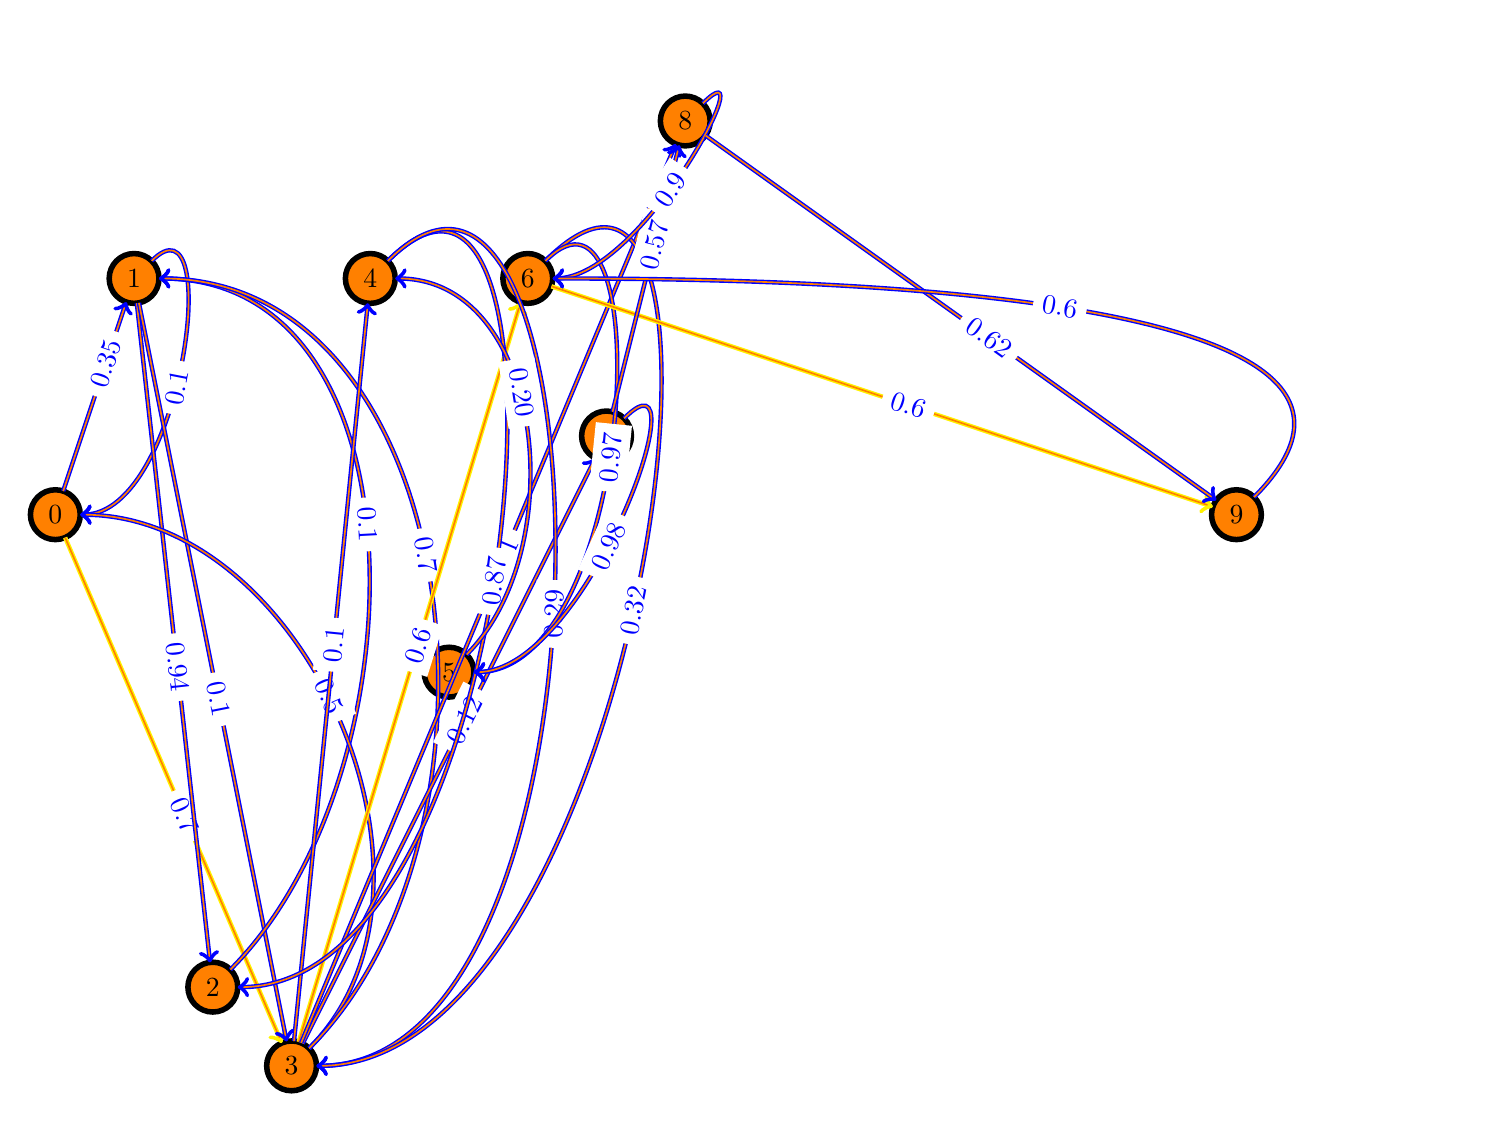
\begin{tikzpicture}
\SetVertexNormal[Shape      = circle,
FillColor  = orange,
LineWidth  = 2pt]
\SetUpEdge[lw         = 0.5pt,
color      = black,
labelcolor = white,
labeltext  = red,
labelstyle = {sloped,text=blue}]
\tikzstyle{TempStyle}=[double = orange]
\Vertex[x=-10, y=8]{0}
\Vertex[x=-9, y=11]{1}
\Vertex[x=-8, y=2]{2}
\Vertex[x=-7, y=1]{3}
\Vertex[x=-6, y=11]{4}
\Vertex[x=-5, y=6]{5}
\Vertex[x=-4, y=11]{6}
\Vertex[x=-3, y=9]{7}
\Vertex[x=-2, y=13]{8}
\Vertex[x=5, y=8]{9}
\tikzset{EdgeStyle/.style={->,TempStyle,relative=false,right=60,color=blue}}
\Edge[label=$0.35$](0)(1)
\tikzset{EdgeStyle/.style={->,TempStyle,relative=false,right=60,color=yellow}}
\Edge[label=$0.7$](0)(3)
\tikzset{EdgeStyle/.style={->,TempStyle,relative=false,left=60,color=blue,in=0,draw}}
\Edge[label=$0.1$](1)(0)
\tikzset{EdgeStyle/.style={->,TempStyle,relative=false,right=60,color=blue}}
\Edge[label=$0.94$](1)(2)
\tikzset{EdgeStyle/.style={->,TempStyle,relative=false,right=60,color=blue}}
\Edge[label=$0.1$](1)(3)
\tikzset{EdgeStyle/.style={->,TempStyle,relative=false,left=60,color=blue,in=0,draw}}
\Edge[label=$0.1$](2)(1)
\tikzset{EdgeStyle/.style={->,TempStyle,relative=false,left=60,color=blue,in=0,draw}}
\Edge[label=$0.5$](3)(0)
\tikzset{EdgeStyle/.style={->,TempStyle,relative=false,left=60,color=blue,in=0,draw}}
\Edge[label=$0.7$](3)(1)
\tikzset{EdgeStyle/.style={->,TempStyle,relative=false,right=60,color=blue}}
\Edge[label=$0.1$](3)(4)
\tikzset{EdgeStyle/.style={->,TempStyle,relative=false,right=60,color=yellow}}
\Edge[label=$0.6$](3)(6)
\tikzset{EdgeStyle/.style={->,TempStyle,relative=false,right=60,color=blue}}
\Edge[label=$0.12$](3)(7)
\tikzset{EdgeStyle/.style={->,TempStyle,relative=false,right=60,color=blue}}
\Edge[label=$0.61$](3)(8)
\tikzset{EdgeStyle/.style={->,TempStyle,relative=false,left=60,color=blue,in=0,draw}}
\Edge[label=$0.87$](4)(2)
\tikzset{EdgeStyle/.style={->,TempStyle,relative=false,left=60,color=blue,in=0,draw}}
\Edge[label=$0.29$](4)(3)
\tikzset{EdgeStyle/.style={->,TempStyle,relative=false,left=60,color=blue,in=0,draw}}
\Edge[label=$0.20$](5)(4)
\tikzset{EdgeStyle/.style={->,TempStyle,relative=false,left=60,color=blue,in=0,draw}}
\Edge[label=$0.32$](6)(3)
\tikzset{EdgeStyle/.style={->,TempStyle,relative=false,left=60,color=blue,in=0,draw}}
\Edge[label=$0.97$](6)(5)
\tikzset{EdgeStyle/.style={->,TempStyle,relative=false,right=60,color=yellow}}
\Edge[label=$0.6$](6)(9)
\tikzset{EdgeStyle/.style={->,TempStyle,relative=false,left=60,color=blue,in=0,draw}}
\Edge[label=$0.98$](7)(5)
\tikzset{EdgeStyle/.style={->,TempStyle,relative=false,right=60,color=blue}}
\Edge[label=$0.57$](7)(8)
\tikzset{EdgeStyle/.style={->,TempStyle,relative=false,left=60,color=blue,in=0,draw}}
\Edge[label=$0.9$](8)(6)
\tikzset{EdgeStyle/.style={->,TempStyle,relative=false,right=60,color=blue}}
\Edge[label=$0.62$](8)(9)
\tikzset{EdgeStyle/.style={->,TempStyle,relative=false,left=60,color=blue,in=0,draw}}
\Edge[label=$0.6$](9)(6)
\end{tikzpicture}\\
\begin{center}\begin{tabular}{l c}\\
\textcolor{orange}{\LARGE$\rightarrow$} & Chemin \\
 \textcolor{red}{\LARGE$\rightarrow$} & Créations arcs\\
 \textcolor{green}{\LARGE$\rightarrow$} & Modification flot\\
\end{tabular}
\end{center}
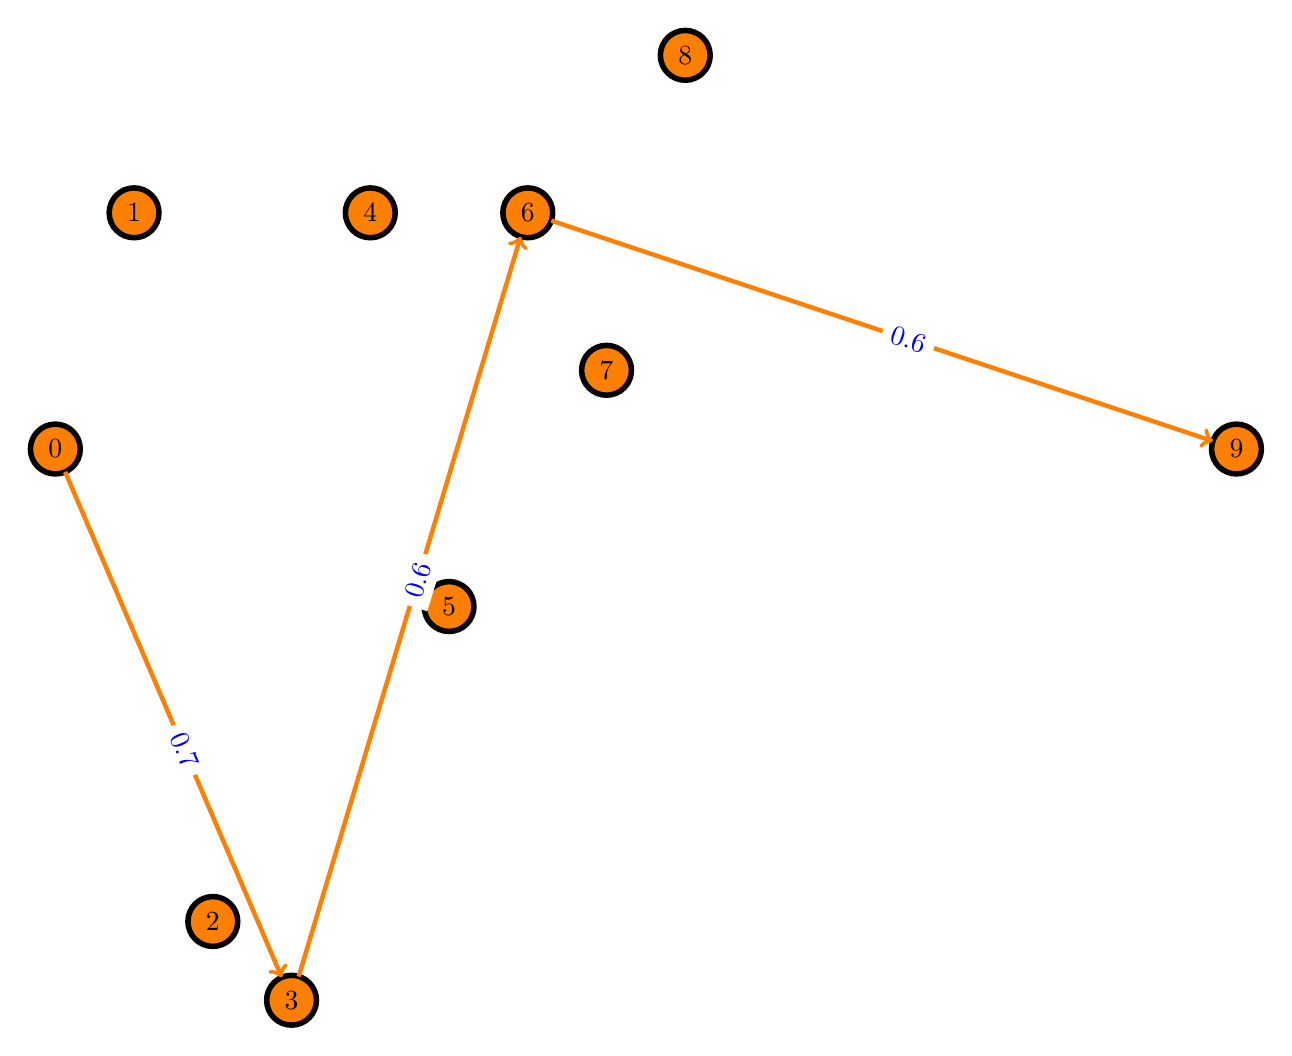
\begin{tikzpicture}
\SetVertexNormal[Shape      = circle,
FillColor  = orange,
LineWidth  = 2pt]
\SetUpEdge[lw         = 0.5pt,
color      = black,
labelcolor = white,
labeltext  = red,
labelstyle = {sloped,text=blue}]
\tikzstyle{TempStyle}=[double = orange]
\Vertex[x=-10, y=8]{0}
\Vertex[x=-9, y=11]{1}
\Vertex[x=-8, y=2]{2}
\Vertex[x=-7, y=1]{3}
\Vertex[x=-6, y=11]{4}
\Vertex[x=-5, y=6]{5}
\Vertex[x=-4, y=11]{6}
\Vertex[x=-3, y=9]{7}
\Vertex[x=-2, y=13]{8}
\Vertex[x=5, y=8]{9}
\tikzset{EdgeStyle/.style={->,TempStyle,relative=false,right=60,color=orange}}
\Edge[label=$0.7$](0)(3)
\tikzset{EdgeStyle/.style={->,TempStyle,relative=false,right=60,color=orange}}
\Edge[label=$0.6$](3)(6)
\tikzset{EdgeStyle/.style={->,TempStyle,relative=false,right=60,color=orange}}
\Edge[label=$0.6$](6)(9)
\end{tikzpicture}\\
\begin{center}\begin{tabular}{l c}\\
\textcolor{orange}{\LARGE$\rightarrow$} & Chemin \\
 \textcolor{red}{\LARGE$\rightarrow$} & Créations arcs\\
 \textcolor{green}{\LARGE$\rightarrow$} & Modification flot\\
\end{tabular}
\end{center}
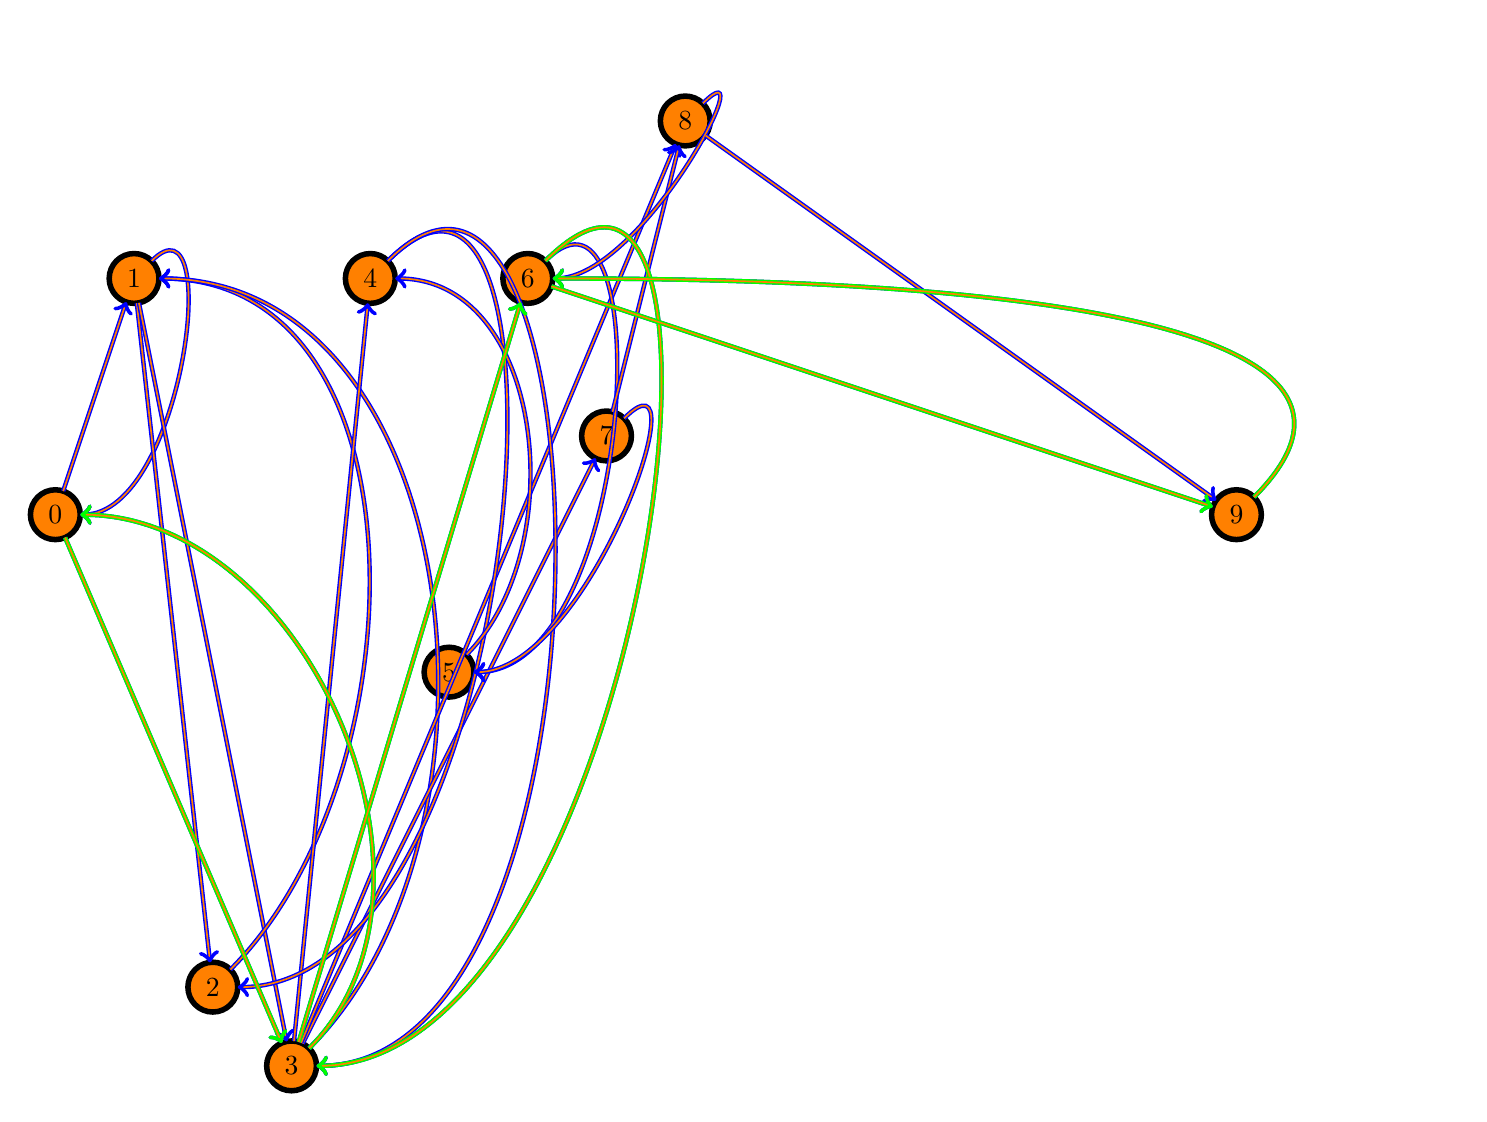
\begin{tikzpicture}
\SetVertexNormal[Shape      = circle,
FillColor  = orange,
LineWidth  = 2pt]
\SetUpEdge[lw         = 0.5pt,
color      = black,
labelcolor = white,
labeltext  = red,
labelstyle = {sloped,text=blue}]
\tikzstyle{TempStyle}=[double = orange]
\Vertex[x=-10, y=8]{0}
\Vertex[x=-9, y=11]{1}
\Vertex[x=-8, y=2]{2}
\Vertex[x=-7, y=1]{3}
\Vertex[x=-6, y=11]{4}
\Vertex[x=-5, y=6]{5}
\Vertex[x=-4, y=11]{6}
\Vertex[x=-3, y=9]{7}
\Vertex[x=-2, y=13]{8}
\Vertex[x=5, y=8]{9}
\tikzset{EdgeStyle/.style={->,TempStyle,relative=false,right=60,color=blue}}
\Edge(0)(1)
\tikzset{EdgeStyle/.style={->,TempStyle,relative=false,right=60,color=blue}}
\Edge(0)(3)
\tikzset{EdgeStyle/.style={->,TempStyle,relative=false,left=60,color=blue,in=0,draw}}
\Edge(1)(0)
\tikzset{EdgeStyle/.style={->,TempStyle,relative=false,right=60,color=blue}}
\Edge(1)(2)
\tikzset{EdgeStyle/.style={->,TempStyle,relative=false,right=60,color=blue}}
\Edge(1)(3)
\tikzset{EdgeStyle/.style={->,TempStyle,relative=false,left=60,color=blue,in=0,draw}}
\Edge(2)(1)
\tikzset{EdgeStyle/.style={->,TempStyle,relative=false,left=60,color=blue,in=0,draw}}
\Edge(3)(0)
\tikzset{EdgeStyle/.style={->,TempStyle,relative=false,left=60,color=blue,in=0,draw}}
\Edge(3)(1)
\tikzset{EdgeStyle/.style={->,TempStyle,relative=false,right=60,color=blue}}
\Edge(3)(4)
\tikzset{EdgeStyle/.style={->,TempStyle,relative=false,right=60,color=blue}}
\Edge(3)(6)
\tikzset{EdgeStyle/.style={->,TempStyle,relative=false,right=60,color=blue}}
\Edge(3)(7)
\tikzset{EdgeStyle/.style={->,TempStyle,relative=false,right=60,color=blue}}
\Edge(3)(8)
\tikzset{EdgeStyle/.style={->,TempStyle,relative=false,left=60,color=blue,in=0,draw}}
\Edge(4)(2)
\tikzset{EdgeStyle/.style={->,TempStyle,relative=false,left=60,color=blue,in=0,draw}}
\Edge(4)(3)
\tikzset{EdgeStyle/.style={->,TempStyle,relative=false,left=60,color=blue,in=0,draw}}
\Edge(5)(4)
\tikzset{EdgeStyle/.style={->,TempStyle,relative=false,left=60,color=blue,in=0,draw}}
\Edge(6)(3)
\tikzset{EdgeStyle/.style={->,TempStyle,relative=false,left=60,color=blue,in=0,draw}}
\Edge(6)(5)
\tikzset{EdgeStyle/.style={->,TempStyle,relative=false,right=60,color=blue}}
\Edge(6)(9)
\tikzset{EdgeStyle/.style={->,TempStyle,relative=false,left=60,color=blue,in=0,draw}}
\Edge(7)(5)
\tikzset{EdgeStyle/.style={->,TempStyle,relative=false,right=60,color=blue}}
\Edge(7)(8)
\tikzset{EdgeStyle/.style={->,TempStyle,relative=false,left=60,color=blue,in=0,draw}}
\Edge(8)(6)
\tikzset{EdgeStyle/.style={->,TempStyle,relative=false,right=60,color=blue}}
\Edge(8)(9)
\tikzset{EdgeStyle/.style={->,TempStyle,relative=false,left=60,color=blue,in=0,draw}}
\Edge(9)(6)
\tikzset{EdgeStyle/.style={->,TempStyle,relative=false,right=60,color=green}}
\Edge(0)(3)
\tikzset{EdgeStyle/.style={->,TempStyle,relative=false,right=60,in=0,color=green}}
\Edge(3)(0)
\tikzset{EdgeStyle/.style={->,TempStyle,relative=false,right=60,color=green}}
\Edge(3)(6)
\tikzset{EdgeStyle/.style={->,TempStyle,relative=false,right=60,in=0,color=green}}
\Edge(6)(3)
\tikzset{EdgeStyle/.style={->,TempStyle,relative=false,right=60,color=green}}
\Edge(6)(9)
\tikzset{EdgeStyle/.style={->,TempStyle,relative=false,right=60,in=0,color=green}}
\Edge(9)(6)
\end{tikzpicture}\\
\begin{center}\begin{tabular}{l c}\\
\textcolor{orange}{\LARGE$\rightarrow$} & Chemin \\
 \textcolor{red}{\LARGE$\rightarrow$} & Créations arcs\\
 \textcolor{green}{\LARGE$\rightarrow$} & Modification flot\\
\end{tabular}
\end{center}
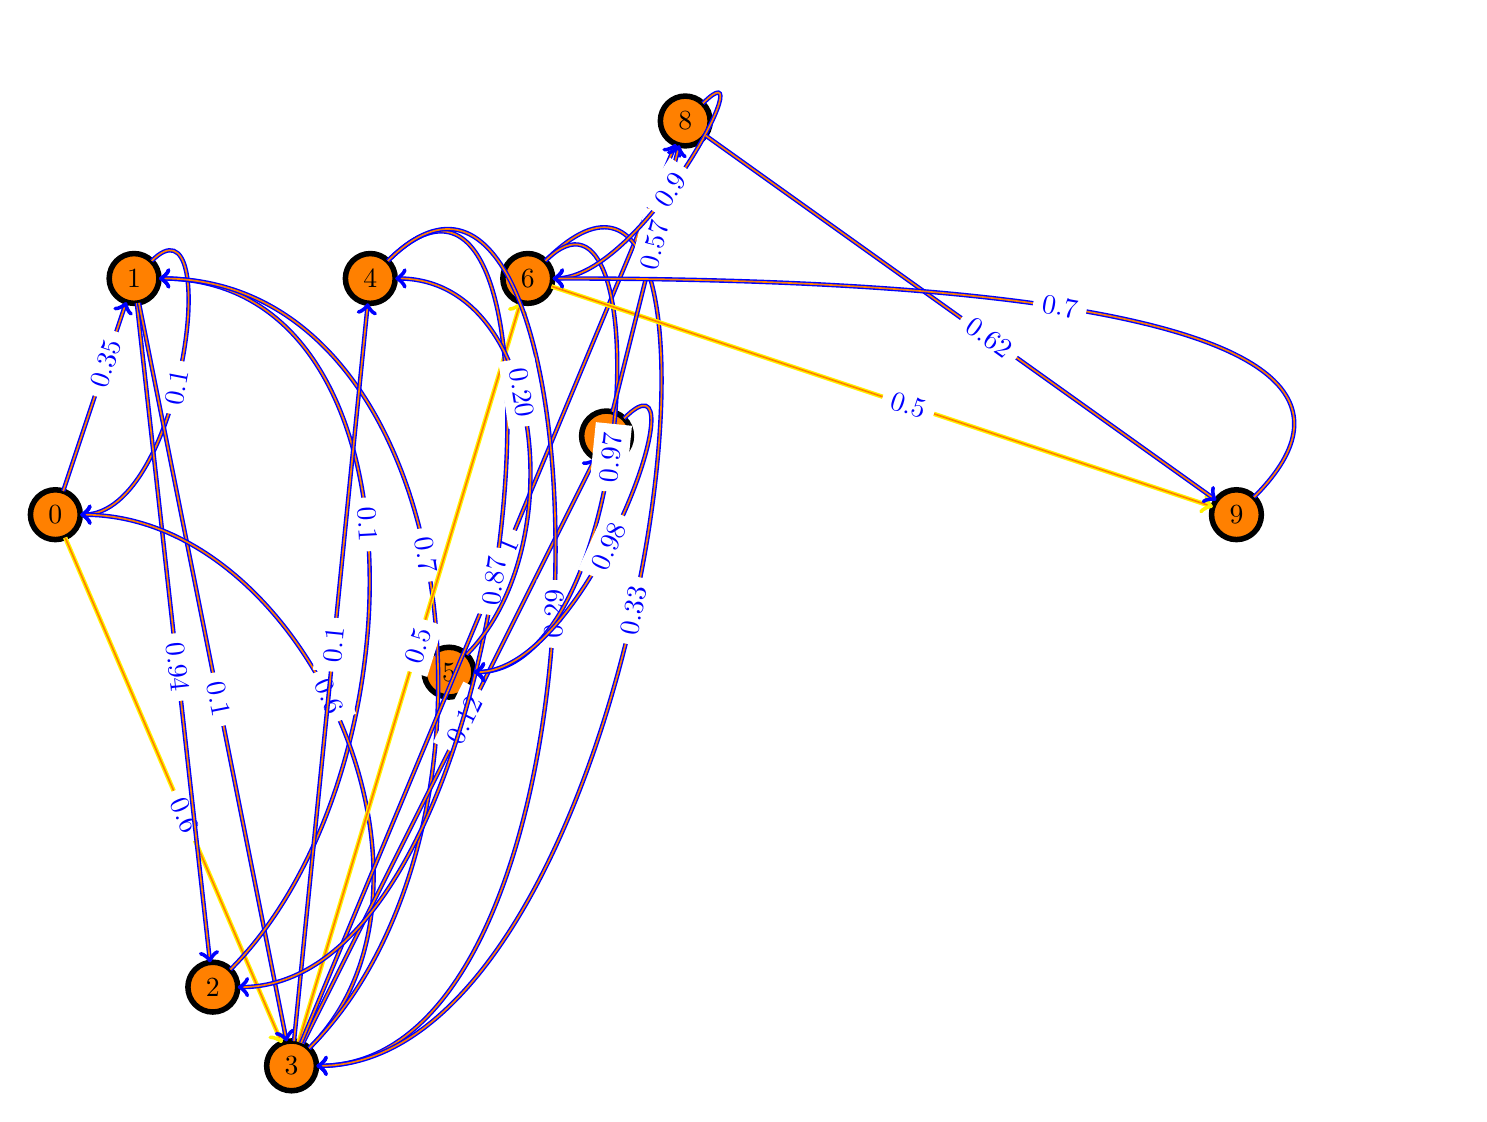
\begin{tikzpicture}
\SetVertexNormal[Shape      = circle,
FillColor  = orange,
LineWidth  = 2pt]
\SetUpEdge[lw         = 0.5pt,
color      = black,
labelcolor = white,
labeltext  = red,
labelstyle = {sloped,text=blue}]
\tikzstyle{TempStyle}=[double = orange]
\Vertex[x=-10, y=8]{0}
\Vertex[x=-9, y=11]{1}
\Vertex[x=-8, y=2]{2}
\Vertex[x=-7, y=1]{3}
\Vertex[x=-6, y=11]{4}
\Vertex[x=-5, y=6]{5}
\Vertex[x=-4, y=11]{6}
\Vertex[x=-3, y=9]{7}
\Vertex[x=-2, y=13]{8}
\Vertex[x=5, y=8]{9}
\tikzset{EdgeStyle/.style={->,TempStyle,relative=false,right=60,color=blue}}
\Edge[label=$0.35$](0)(1)
\tikzset{EdgeStyle/.style={->,TempStyle,relative=false,right=60,color=yellow}}
\Edge[label=$0.6$](0)(3)
\tikzset{EdgeStyle/.style={->,TempStyle,relative=false,left=60,color=blue,in=0,draw}}
\Edge[label=$0.1$](1)(0)
\tikzset{EdgeStyle/.style={->,TempStyle,relative=false,right=60,color=blue}}
\Edge[label=$0.94$](1)(2)
\tikzset{EdgeStyle/.style={->,TempStyle,relative=false,right=60,color=blue}}
\Edge[label=$0.1$](1)(3)
\tikzset{EdgeStyle/.style={->,TempStyle,relative=false,left=60,color=blue,in=0,draw}}
\Edge[label=$0.1$](2)(1)
\tikzset{EdgeStyle/.style={->,TempStyle,relative=false,left=60,color=blue,in=0,draw}}
\Edge[label=$0.6$](3)(0)
\tikzset{EdgeStyle/.style={->,TempStyle,relative=false,left=60,color=blue,in=0,draw}}
\Edge[label=$0.7$](3)(1)
\tikzset{EdgeStyle/.style={->,TempStyle,relative=false,right=60,color=blue}}
\Edge[label=$0.1$](3)(4)
\tikzset{EdgeStyle/.style={->,TempStyle,relative=false,right=60,color=yellow}}
\Edge[label=$0.5$](3)(6)
\tikzset{EdgeStyle/.style={->,TempStyle,relative=false,right=60,color=blue}}
\Edge[label=$0.12$](3)(7)
\tikzset{EdgeStyle/.style={->,TempStyle,relative=false,right=60,color=blue}}
\Edge[label=$0.61$](3)(8)
\tikzset{EdgeStyle/.style={->,TempStyle,relative=false,left=60,color=blue,in=0,draw}}
\Edge[label=$0.87$](4)(2)
\tikzset{EdgeStyle/.style={->,TempStyle,relative=false,left=60,color=blue,in=0,draw}}
\Edge[label=$0.29$](4)(3)
\tikzset{EdgeStyle/.style={->,TempStyle,relative=false,left=60,color=blue,in=0,draw}}
\Edge[label=$0.20$](5)(4)
\tikzset{EdgeStyle/.style={->,TempStyle,relative=false,left=60,color=blue,in=0,draw}}
\Edge[label=$0.33$](6)(3)
\tikzset{EdgeStyle/.style={->,TempStyle,relative=false,left=60,color=blue,in=0,draw}}
\Edge[label=$0.97$](6)(5)
\tikzset{EdgeStyle/.style={->,TempStyle,relative=false,right=60,color=yellow}}
\Edge[label=$0.5$](6)(9)
\tikzset{EdgeStyle/.style={->,TempStyle,relative=false,left=60,color=blue,in=0,draw}}
\Edge[label=$0.98$](7)(5)
\tikzset{EdgeStyle/.style={->,TempStyle,relative=false,right=60,color=blue}}
\Edge[label=$0.57$](7)(8)
\tikzset{EdgeStyle/.style={->,TempStyle,relative=false,left=60,color=blue,in=0,draw}}
\Edge[label=$0.9$](8)(6)
\tikzset{EdgeStyle/.style={->,TempStyle,relative=false,right=60,color=blue}}
\Edge[label=$0.62$](8)(9)
\tikzset{EdgeStyle/.style={->,TempStyle,relative=false,left=60,color=blue,in=0,draw}}
\Edge[label=$0.7$](9)(6)
\end{tikzpicture}\\
\begin{center}\begin{tabular}{l c}\\
\textcolor{orange}{\LARGE$\rightarrow$} & Chemin \\
 \textcolor{red}{\LARGE$\rightarrow$} & Créations arcs\\
 \textcolor{green}{\LARGE$\rightarrow$} & Modification flot\\
\end{tabular}
\end{center}
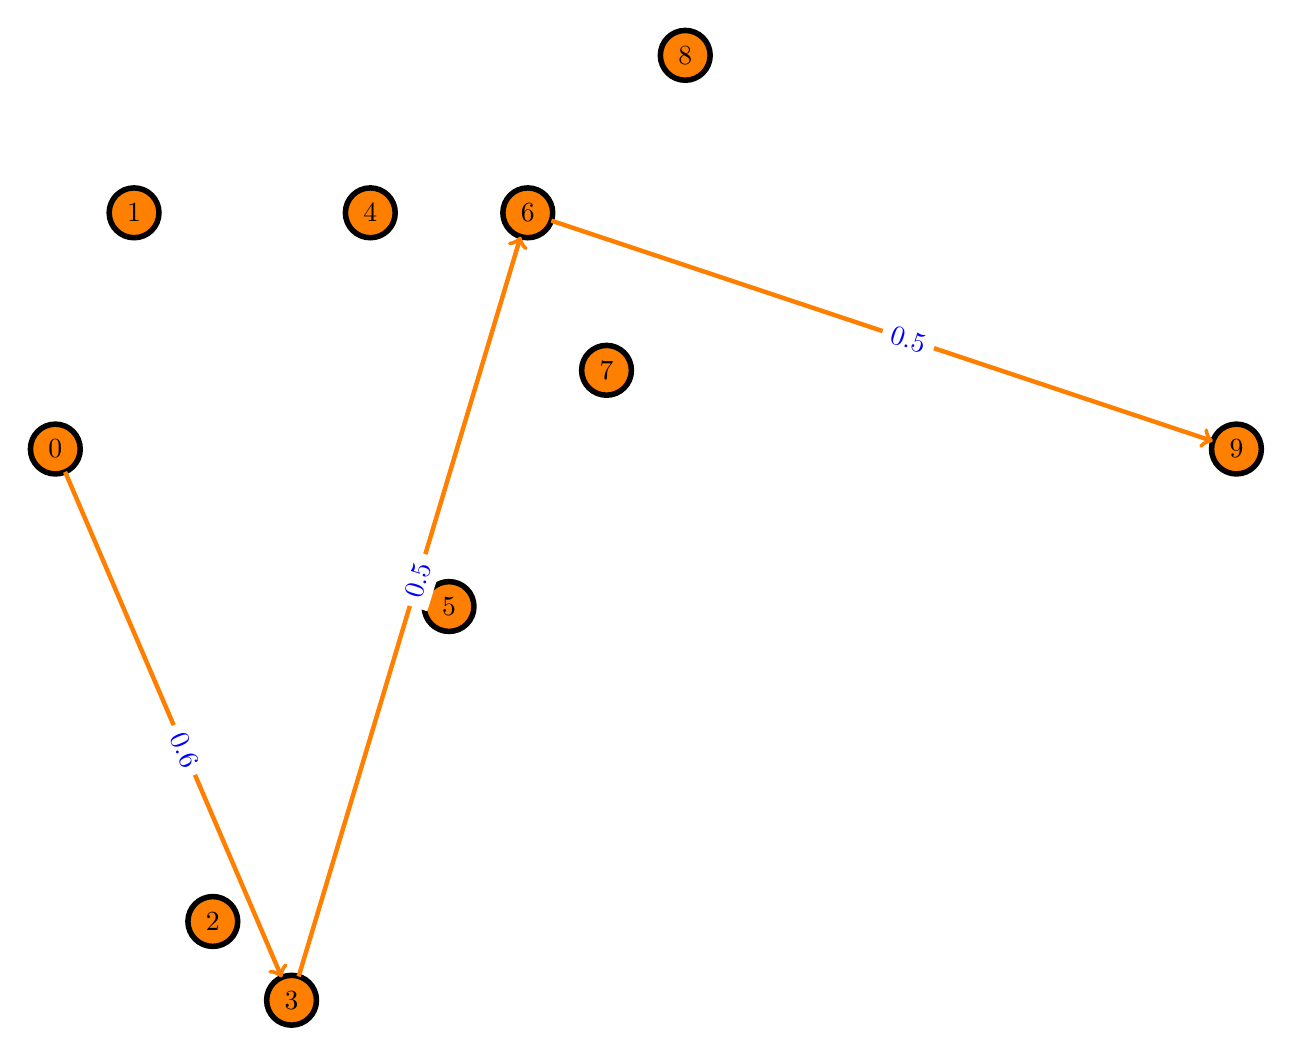
\begin{tikzpicture}
\SetVertexNormal[Shape      = circle,
FillColor  = orange,
LineWidth  = 2pt]
\SetUpEdge[lw         = 0.5pt,
color      = black,
labelcolor = white,
labeltext  = red,
labelstyle = {sloped,text=blue}]
\tikzstyle{TempStyle}=[double = orange]
\Vertex[x=-10, y=8]{0}
\Vertex[x=-9, y=11]{1}
\Vertex[x=-8, y=2]{2}
\Vertex[x=-7, y=1]{3}
\Vertex[x=-6, y=11]{4}
\Vertex[x=-5, y=6]{5}
\Vertex[x=-4, y=11]{6}
\Vertex[x=-3, y=9]{7}
\Vertex[x=-2, y=13]{8}
\Vertex[x=5, y=8]{9}
\tikzset{EdgeStyle/.style={->,TempStyle,relative=false,right=60,color=orange}}
\Edge[label=$0.6$](0)(3)
\tikzset{EdgeStyle/.style={->,TempStyle,relative=false,right=60,color=orange}}
\Edge[label=$0.5$](3)(6)
\tikzset{EdgeStyle/.style={->,TempStyle,relative=false,right=60,color=orange}}
\Edge[label=$0.5$](6)(9)
\end{tikzpicture}\\
\begin{center}\begin{tabular}{l c}\\
\textcolor{orange}{\LARGE$\rightarrow$} & Chemin \\
 \textcolor{red}{\LARGE$\rightarrow$} & Créations arcs\\
 \textcolor{green}{\LARGE$\rightarrow$} & Modification flot\\
\end{tabular}
\end{center}
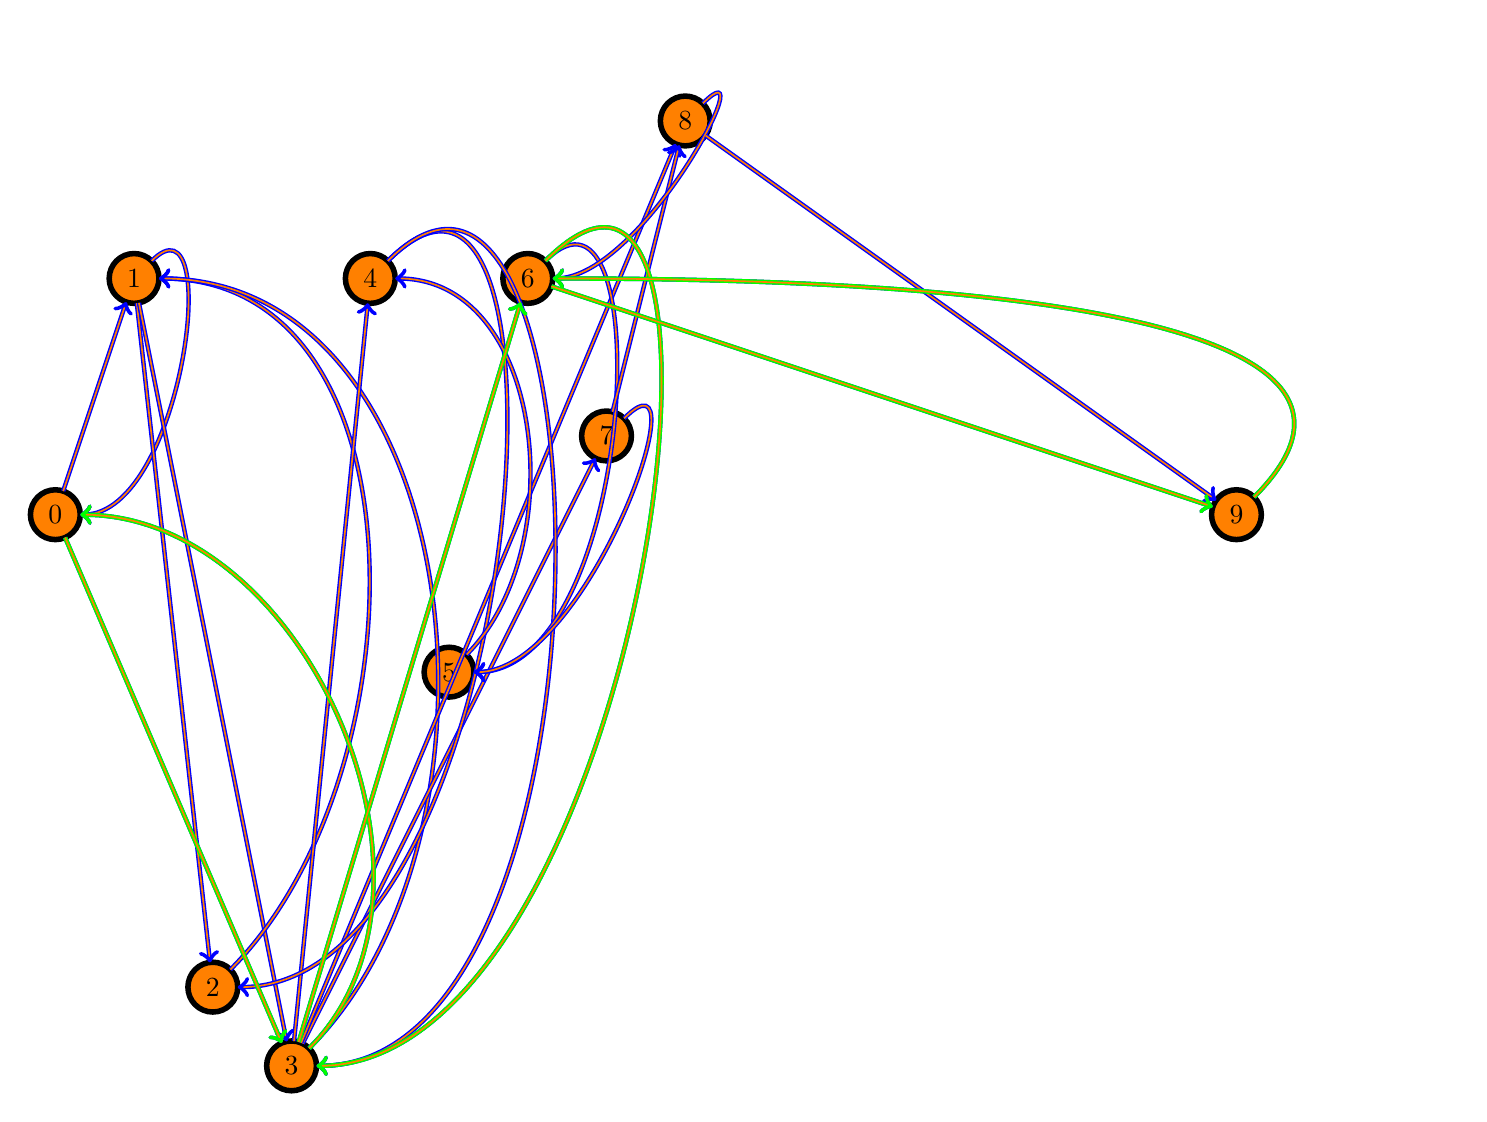
\begin{tikzpicture}
\SetVertexNormal[Shape      = circle,
FillColor  = orange,
LineWidth  = 2pt]
\SetUpEdge[lw         = 0.5pt,
color      = black,
labelcolor = white,
labeltext  = red,
labelstyle = {sloped,text=blue}]
\tikzstyle{TempStyle}=[double = orange]
\Vertex[x=-10, y=8]{0}
\Vertex[x=-9, y=11]{1}
\Vertex[x=-8, y=2]{2}
\Vertex[x=-7, y=1]{3}
\Vertex[x=-6, y=11]{4}
\Vertex[x=-5, y=6]{5}
\Vertex[x=-4, y=11]{6}
\Vertex[x=-3, y=9]{7}
\Vertex[x=-2, y=13]{8}
\Vertex[x=5, y=8]{9}
\tikzset{EdgeStyle/.style={->,TempStyle,relative=false,right=60,color=blue}}
\Edge(0)(1)
\tikzset{EdgeStyle/.style={->,TempStyle,relative=false,right=60,color=blue}}
\Edge(0)(3)
\tikzset{EdgeStyle/.style={->,TempStyle,relative=false,left=60,color=blue,in=0,draw}}
\Edge(1)(0)
\tikzset{EdgeStyle/.style={->,TempStyle,relative=false,right=60,color=blue}}
\Edge(1)(2)
\tikzset{EdgeStyle/.style={->,TempStyle,relative=false,right=60,color=blue}}
\Edge(1)(3)
\tikzset{EdgeStyle/.style={->,TempStyle,relative=false,left=60,color=blue,in=0,draw}}
\Edge(2)(1)
\tikzset{EdgeStyle/.style={->,TempStyle,relative=false,left=60,color=blue,in=0,draw}}
\Edge(3)(0)
\tikzset{EdgeStyle/.style={->,TempStyle,relative=false,left=60,color=blue,in=0,draw}}
\Edge(3)(1)
\tikzset{EdgeStyle/.style={->,TempStyle,relative=false,right=60,color=blue}}
\Edge(3)(4)
\tikzset{EdgeStyle/.style={->,TempStyle,relative=false,right=60,color=blue}}
\Edge(3)(6)
\tikzset{EdgeStyle/.style={->,TempStyle,relative=false,right=60,color=blue}}
\Edge(3)(7)
\tikzset{EdgeStyle/.style={->,TempStyle,relative=false,right=60,color=blue}}
\Edge(3)(8)
\tikzset{EdgeStyle/.style={->,TempStyle,relative=false,left=60,color=blue,in=0,draw}}
\Edge(4)(2)
\tikzset{EdgeStyle/.style={->,TempStyle,relative=false,left=60,color=blue,in=0,draw}}
\Edge(4)(3)
\tikzset{EdgeStyle/.style={->,TempStyle,relative=false,left=60,color=blue,in=0,draw}}
\Edge(5)(4)
\tikzset{EdgeStyle/.style={->,TempStyle,relative=false,left=60,color=blue,in=0,draw}}
\Edge(6)(3)
\tikzset{EdgeStyle/.style={->,TempStyle,relative=false,left=60,color=blue,in=0,draw}}
\Edge(6)(5)
\tikzset{EdgeStyle/.style={->,TempStyle,relative=false,right=60,color=blue}}
\Edge(6)(9)
\tikzset{EdgeStyle/.style={->,TempStyle,relative=false,left=60,color=blue,in=0,draw}}
\Edge(7)(5)
\tikzset{EdgeStyle/.style={->,TempStyle,relative=false,right=60,color=blue}}
\Edge(7)(8)
\tikzset{EdgeStyle/.style={->,TempStyle,relative=false,left=60,color=blue,in=0,draw}}
\Edge(8)(6)
\tikzset{EdgeStyle/.style={->,TempStyle,relative=false,right=60,color=blue}}
\Edge(8)(9)
\tikzset{EdgeStyle/.style={->,TempStyle,relative=false,left=60,color=blue,in=0,draw}}
\Edge(9)(6)
\tikzset{EdgeStyle/.style={->,TempStyle,relative=false,right=60,color=green}}
\Edge(0)(3)
\tikzset{EdgeStyle/.style={->,TempStyle,relative=false,right=60,in=0,color=green}}
\Edge(3)(0)
\tikzset{EdgeStyle/.style={->,TempStyle,relative=false,right=60,color=green}}
\Edge(3)(6)
\tikzset{EdgeStyle/.style={->,TempStyle,relative=false,right=60,in=0,color=green}}
\Edge(6)(3)
\tikzset{EdgeStyle/.style={->,TempStyle,relative=false,right=60,color=green}}
\Edge(6)(9)
\tikzset{EdgeStyle/.style={->,TempStyle,relative=false,right=60,in=0,color=green}}
\Edge(9)(6)
\end{tikzpicture}\\
\begin{center}\begin{tabular}{l c}\\
\textcolor{orange}{\LARGE$\rightarrow$} & Chemin \\
 \textcolor{red}{\LARGE$\rightarrow$} & Créations arcs\\
 \textcolor{green}{\LARGE$\rightarrow$} & Modification flot\\
\end{tabular}
\end{center}
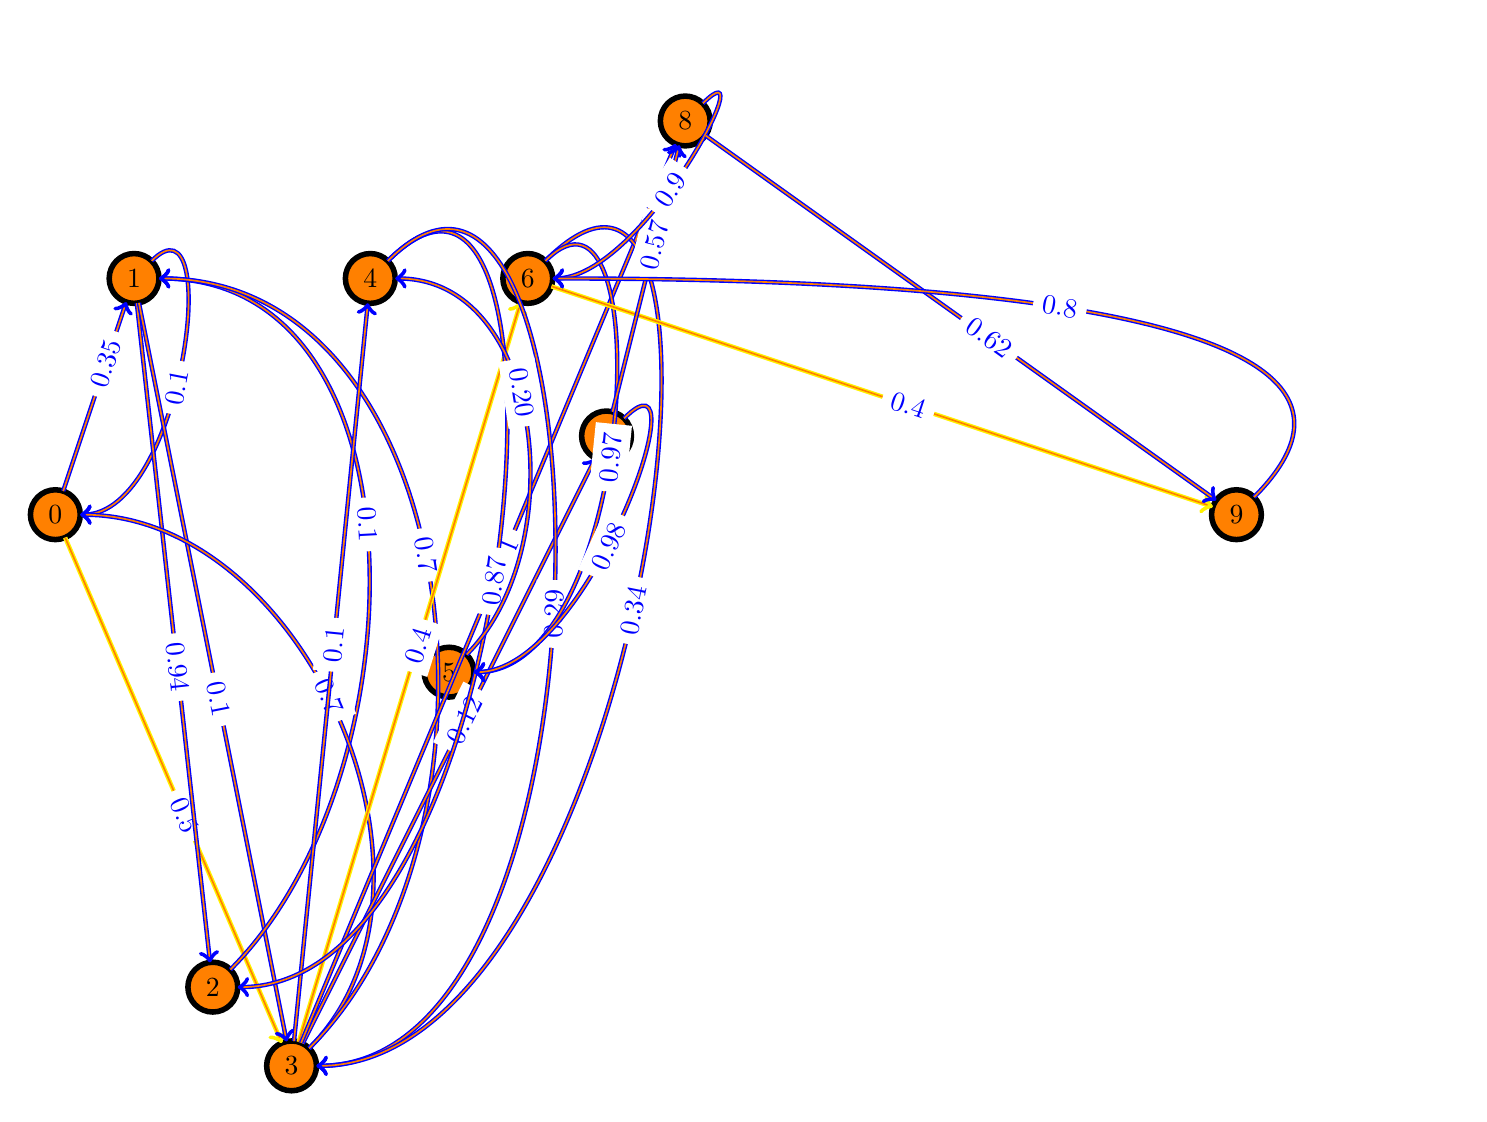
\begin{tikzpicture}
\SetVertexNormal[Shape      = circle,
FillColor  = orange,
LineWidth  = 2pt]
\SetUpEdge[lw         = 0.5pt,
color      = black,
labelcolor = white,
labeltext  = red,
labelstyle = {sloped,text=blue}]
\tikzstyle{TempStyle}=[double = orange]
\Vertex[x=-10, y=8]{0}
\Vertex[x=-9, y=11]{1}
\Vertex[x=-8, y=2]{2}
\Vertex[x=-7, y=1]{3}
\Vertex[x=-6, y=11]{4}
\Vertex[x=-5, y=6]{5}
\Vertex[x=-4, y=11]{6}
\Vertex[x=-3, y=9]{7}
\Vertex[x=-2, y=13]{8}
\Vertex[x=5, y=8]{9}
\tikzset{EdgeStyle/.style={->,TempStyle,relative=false,right=60,color=blue}}
\Edge[label=$0.35$](0)(1)
\tikzset{EdgeStyle/.style={->,TempStyle,relative=false,right=60,color=yellow}}
\Edge[label=$0.5$](0)(3)
\tikzset{EdgeStyle/.style={->,TempStyle,relative=false,left=60,color=blue,in=0,draw}}
\Edge[label=$0.1$](1)(0)
\tikzset{EdgeStyle/.style={->,TempStyle,relative=false,right=60,color=blue}}
\Edge[label=$0.94$](1)(2)
\tikzset{EdgeStyle/.style={->,TempStyle,relative=false,right=60,color=blue}}
\Edge[label=$0.1$](1)(3)
\tikzset{EdgeStyle/.style={->,TempStyle,relative=false,left=60,color=blue,in=0,draw}}
\Edge[label=$0.1$](2)(1)
\tikzset{EdgeStyle/.style={->,TempStyle,relative=false,left=60,color=blue,in=0,draw}}
\Edge[label=$0.7$](3)(0)
\tikzset{EdgeStyle/.style={->,TempStyle,relative=false,left=60,color=blue,in=0,draw}}
\Edge[label=$0.7$](3)(1)
\tikzset{EdgeStyle/.style={->,TempStyle,relative=false,right=60,color=blue}}
\Edge[label=$0.1$](3)(4)
\tikzset{EdgeStyle/.style={->,TempStyle,relative=false,right=60,color=yellow}}
\Edge[label=$0.4$](3)(6)
\tikzset{EdgeStyle/.style={->,TempStyle,relative=false,right=60,color=blue}}
\Edge[label=$0.12$](3)(7)
\tikzset{EdgeStyle/.style={->,TempStyle,relative=false,right=60,color=blue}}
\Edge[label=$0.61$](3)(8)
\tikzset{EdgeStyle/.style={->,TempStyle,relative=false,left=60,color=blue,in=0,draw}}
\Edge[label=$0.87$](4)(2)
\tikzset{EdgeStyle/.style={->,TempStyle,relative=false,left=60,color=blue,in=0,draw}}
\Edge[label=$0.29$](4)(3)
\tikzset{EdgeStyle/.style={->,TempStyle,relative=false,left=60,color=blue,in=0,draw}}
\Edge[label=$0.20$](5)(4)
\tikzset{EdgeStyle/.style={->,TempStyle,relative=false,left=60,color=blue,in=0,draw}}
\Edge[label=$0.34$](6)(3)
\tikzset{EdgeStyle/.style={->,TempStyle,relative=false,left=60,color=blue,in=0,draw}}
\Edge[label=$0.97$](6)(5)
\tikzset{EdgeStyle/.style={->,TempStyle,relative=false,right=60,color=yellow}}
\Edge[label=$0.4$](6)(9)
\tikzset{EdgeStyle/.style={->,TempStyle,relative=false,left=60,color=blue,in=0,draw}}
\Edge[label=$0.98$](7)(5)
\tikzset{EdgeStyle/.style={->,TempStyle,relative=false,right=60,color=blue}}
\Edge[label=$0.57$](7)(8)
\tikzset{EdgeStyle/.style={->,TempStyle,relative=false,left=60,color=blue,in=0,draw}}
\Edge[label=$0.9$](8)(6)
\tikzset{EdgeStyle/.style={->,TempStyle,relative=false,right=60,color=blue}}
\Edge[label=$0.62$](8)(9)
\tikzset{EdgeStyle/.style={->,TempStyle,relative=false,left=60,color=blue,in=0,draw}}
\Edge[label=$0.8$](9)(6)
\end{tikzpicture}\\
\begin{center}\begin{tabular}{l c}\\
\textcolor{orange}{\LARGE$\rightarrow$} & Chemin \\
 \textcolor{red}{\LARGE$\rightarrow$} & Créations arcs\\
 \textcolor{green}{\LARGE$\rightarrow$} & Modification flot\\
\end{tabular}
\end{center}
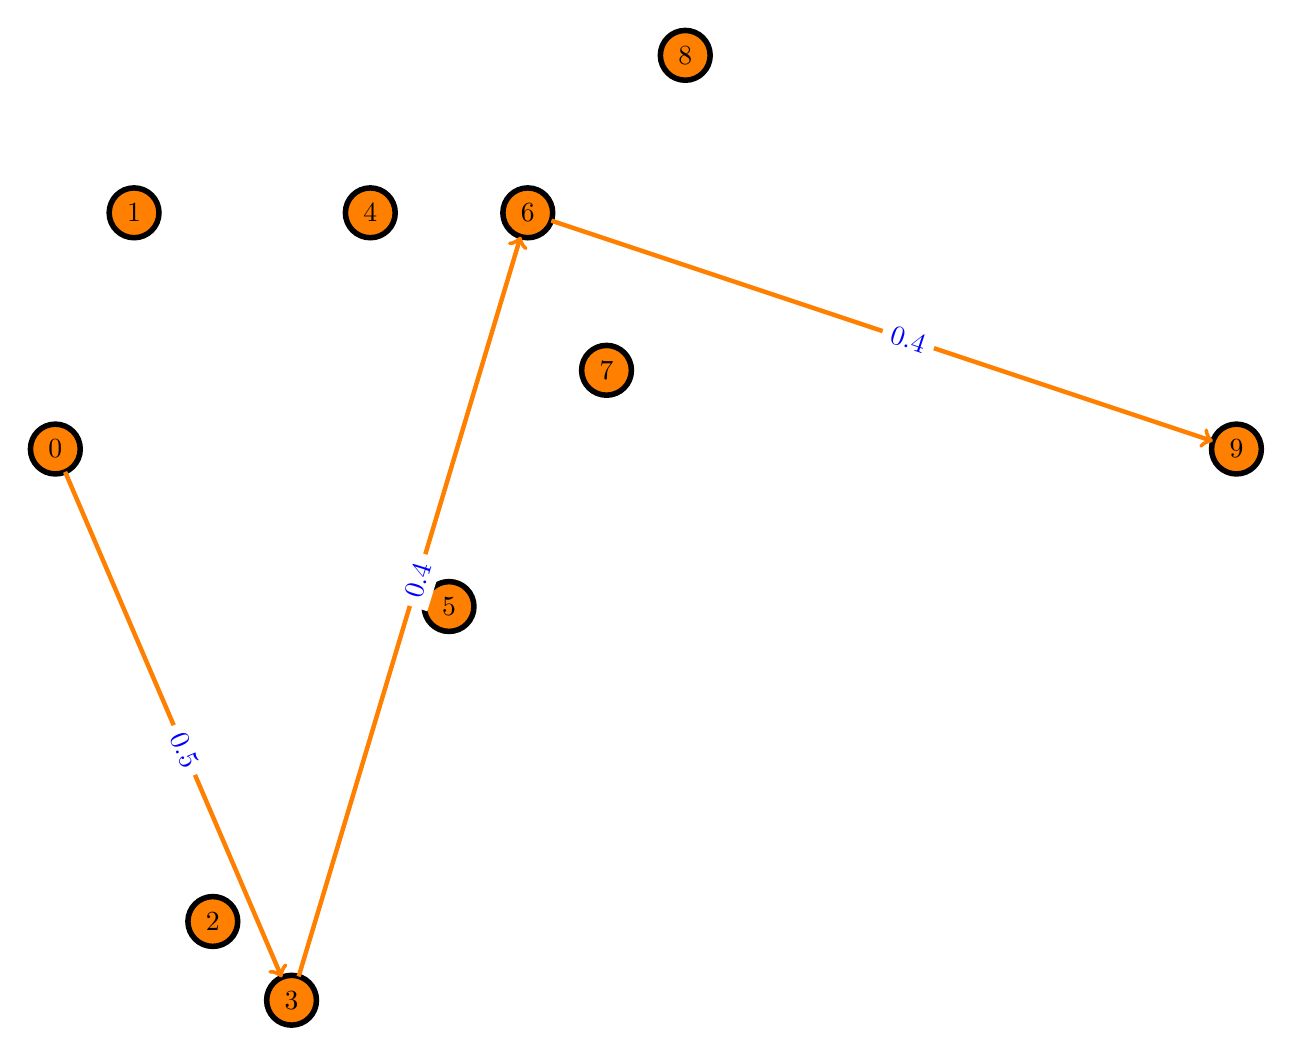
\begin{tikzpicture}
\SetVertexNormal[Shape      = circle,
FillColor  = orange,
LineWidth  = 2pt]
\SetUpEdge[lw         = 0.5pt,
color      = black,
labelcolor = white,
labeltext  = red,
labelstyle = {sloped,text=blue}]
\tikzstyle{TempStyle}=[double = orange]
\Vertex[x=-10, y=8]{0}
\Vertex[x=-9, y=11]{1}
\Vertex[x=-8, y=2]{2}
\Vertex[x=-7, y=1]{3}
\Vertex[x=-6, y=11]{4}
\Vertex[x=-5, y=6]{5}
\Vertex[x=-4, y=11]{6}
\Vertex[x=-3, y=9]{7}
\Vertex[x=-2, y=13]{8}
\Vertex[x=5, y=8]{9}
\tikzset{EdgeStyle/.style={->,TempStyle,relative=false,right=60,color=orange}}
\Edge[label=$0.5$](0)(3)
\tikzset{EdgeStyle/.style={->,TempStyle,relative=false,right=60,color=orange}}
\Edge[label=$0.4$](3)(6)
\tikzset{EdgeStyle/.style={->,TempStyle,relative=false,right=60,color=orange}}
\Edge[label=$0.4$](6)(9)
\end{tikzpicture}\\
\begin{center}\begin{tabular}{l c}\\
\textcolor{orange}{\LARGE$\rightarrow$} & Chemin \\
 \textcolor{red}{\LARGE$\rightarrow$} & Créations arcs\\
 \textcolor{green}{\LARGE$\rightarrow$} & Modification flot\\
\end{tabular}
\end{center}
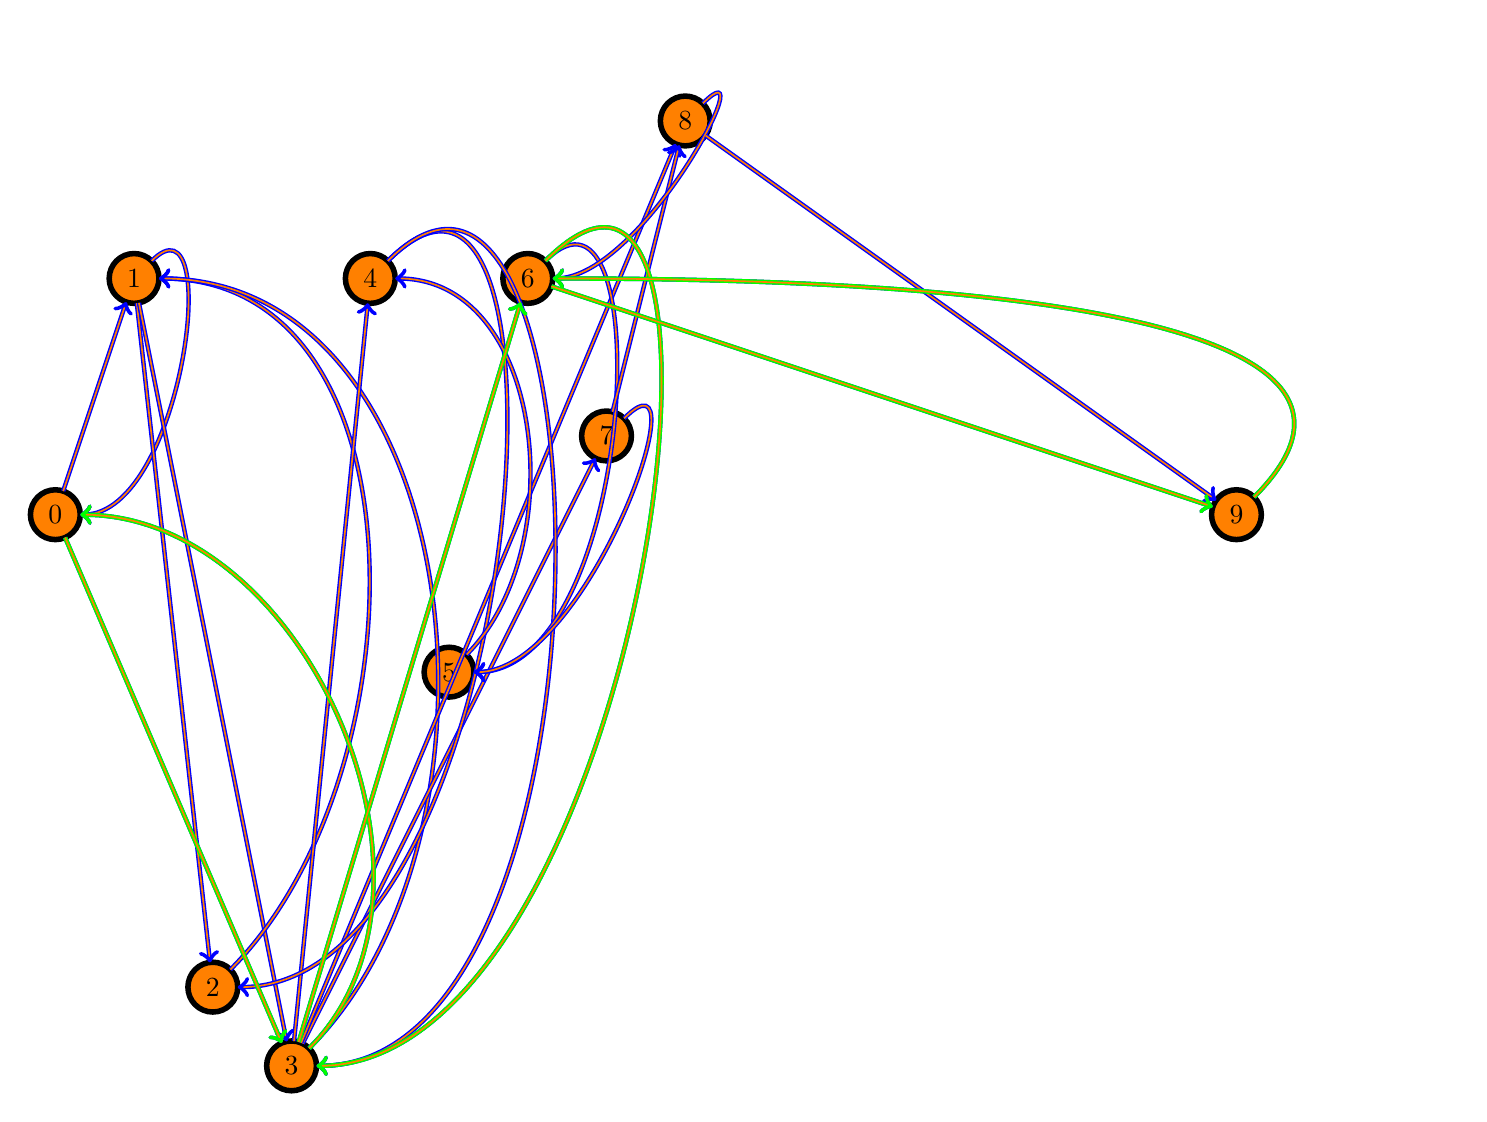
\begin{tikzpicture}
\SetVertexNormal[Shape      = circle,
FillColor  = orange,
LineWidth  = 2pt]
\SetUpEdge[lw         = 0.5pt,
color      = black,
labelcolor = white,
labeltext  = red,
labelstyle = {sloped,text=blue}]
\tikzstyle{TempStyle}=[double = orange]
\Vertex[x=-10, y=8]{0}
\Vertex[x=-9, y=11]{1}
\Vertex[x=-8, y=2]{2}
\Vertex[x=-7, y=1]{3}
\Vertex[x=-6, y=11]{4}
\Vertex[x=-5, y=6]{5}
\Vertex[x=-4, y=11]{6}
\Vertex[x=-3, y=9]{7}
\Vertex[x=-2, y=13]{8}
\Vertex[x=5, y=8]{9}
\tikzset{EdgeStyle/.style={->,TempStyle,relative=false,right=60,color=blue}}
\Edge(0)(1)
\tikzset{EdgeStyle/.style={->,TempStyle,relative=false,right=60,color=blue}}
\Edge(0)(3)
\tikzset{EdgeStyle/.style={->,TempStyle,relative=false,left=60,color=blue,in=0,draw}}
\Edge(1)(0)
\tikzset{EdgeStyle/.style={->,TempStyle,relative=false,right=60,color=blue}}
\Edge(1)(2)
\tikzset{EdgeStyle/.style={->,TempStyle,relative=false,right=60,color=blue}}
\Edge(1)(3)
\tikzset{EdgeStyle/.style={->,TempStyle,relative=false,left=60,color=blue,in=0,draw}}
\Edge(2)(1)
\tikzset{EdgeStyle/.style={->,TempStyle,relative=false,left=60,color=blue,in=0,draw}}
\Edge(3)(0)
\tikzset{EdgeStyle/.style={->,TempStyle,relative=false,left=60,color=blue,in=0,draw}}
\Edge(3)(1)
\tikzset{EdgeStyle/.style={->,TempStyle,relative=false,right=60,color=blue}}
\Edge(3)(4)
\tikzset{EdgeStyle/.style={->,TempStyle,relative=false,right=60,color=blue}}
\Edge(3)(6)
\tikzset{EdgeStyle/.style={->,TempStyle,relative=false,right=60,color=blue}}
\Edge(3)(7)
\tikzset{EdgeStyle/.style={->,TempStyle,relative=false,right=60,color=blue}}
\Edge(3)(8)
\tikzset{EdgeStyle/.style={->,TempStyle,relative=false,left=60,color=blue,in=0,draw}}
\Edge(4)(2)
\tikzset{EdgeStyle/.style={->,TempStyle,relative=false,left=60,color=blue,in=0,draw}}
\Edge(4)(3)
\tikzset{EdgeStyle/.style={->,TempStyle,relative=false,left=60,color=blue,in=0,draw}}
\Edge(5)(4)
\tikzset{EdgeStyle/.style={->,TempStyle,relative=false,left=60,color=blue,in=0,draw}}
\Edge(6)(3)
\tikzset{EdgeStyle/.style={->,TempStyle,relative=false,left=60,color=blue,in=0,draw}}
\Edge(6)(5)
\tikzset{EdgeStyle/.style={->,TempStyle,relative=false,right=60,color=blue}}
\Edge(6)(9)
\tikzset{EdgeStyle/.style={->,TempStyle,relative=false,left=60,color=blue,in=0,draw}}
\Edge(7)(5)
\tikzset{EdgeStyle/.style={->,TempStyle,relative=false,right=60,color=blue}}
\Edge(7)(8)
\tikzset{EdgeStyle/.style={->,TempStyle,relative=false,left=60,color=blue,in=0,draw}}
\Edge(8)(6)
\tikzset{EdgeStyle/.style={->,TempStyle,relative=false,right=60,color=blue}}
\Edge(8)(9)
\tikzset{EdgeStyle/.style={->,TempStyle,relative=false,left=60,color=blue,in=0,draw}}
\Edge(9)(6)
\tikzset{EdgeStyle/.style={->,TempStyle,relative=false,right=60,color=green}}
\Edge(0)(3)
\tikzset{EdgeStyle/.style={->,TempStyle,relative=false,right=60,in=0,color=green}}
\Edge(3)(0)
\tikzset{EdgeStyle/.style={->,TempStyle,relative=false,right=60,color=green}}
\Edge(3)(6)
\tikzset{EdgeStyle/.style={->,TempStyle,relative=false,right=60,in=0,color=green}}
\Edge(6)(3)
\tikzset{EdgeStyle/.style={->,TempStyle,relative=false,right=60,color=green}}
\Edge(6)(9)
\tikzset{EdgeStyle/.style={->,TempStyle,relative=false,right=60,in=0,color=green}}
\Edge(9)(6)
\end{tikzpicture}\\
\begin{center}\begin{tabular}{l c}\\
\textcolor{orange}{\LARGE$\rightarrow$} & Chemin \\
 \textcolor{red}{\LARGE$\rightarrow$} & Créations arcs\\
 \textcolor{green}{\LARGE$\rightarrow$} & Modification flot\\
\end{tabular}
\end{center}
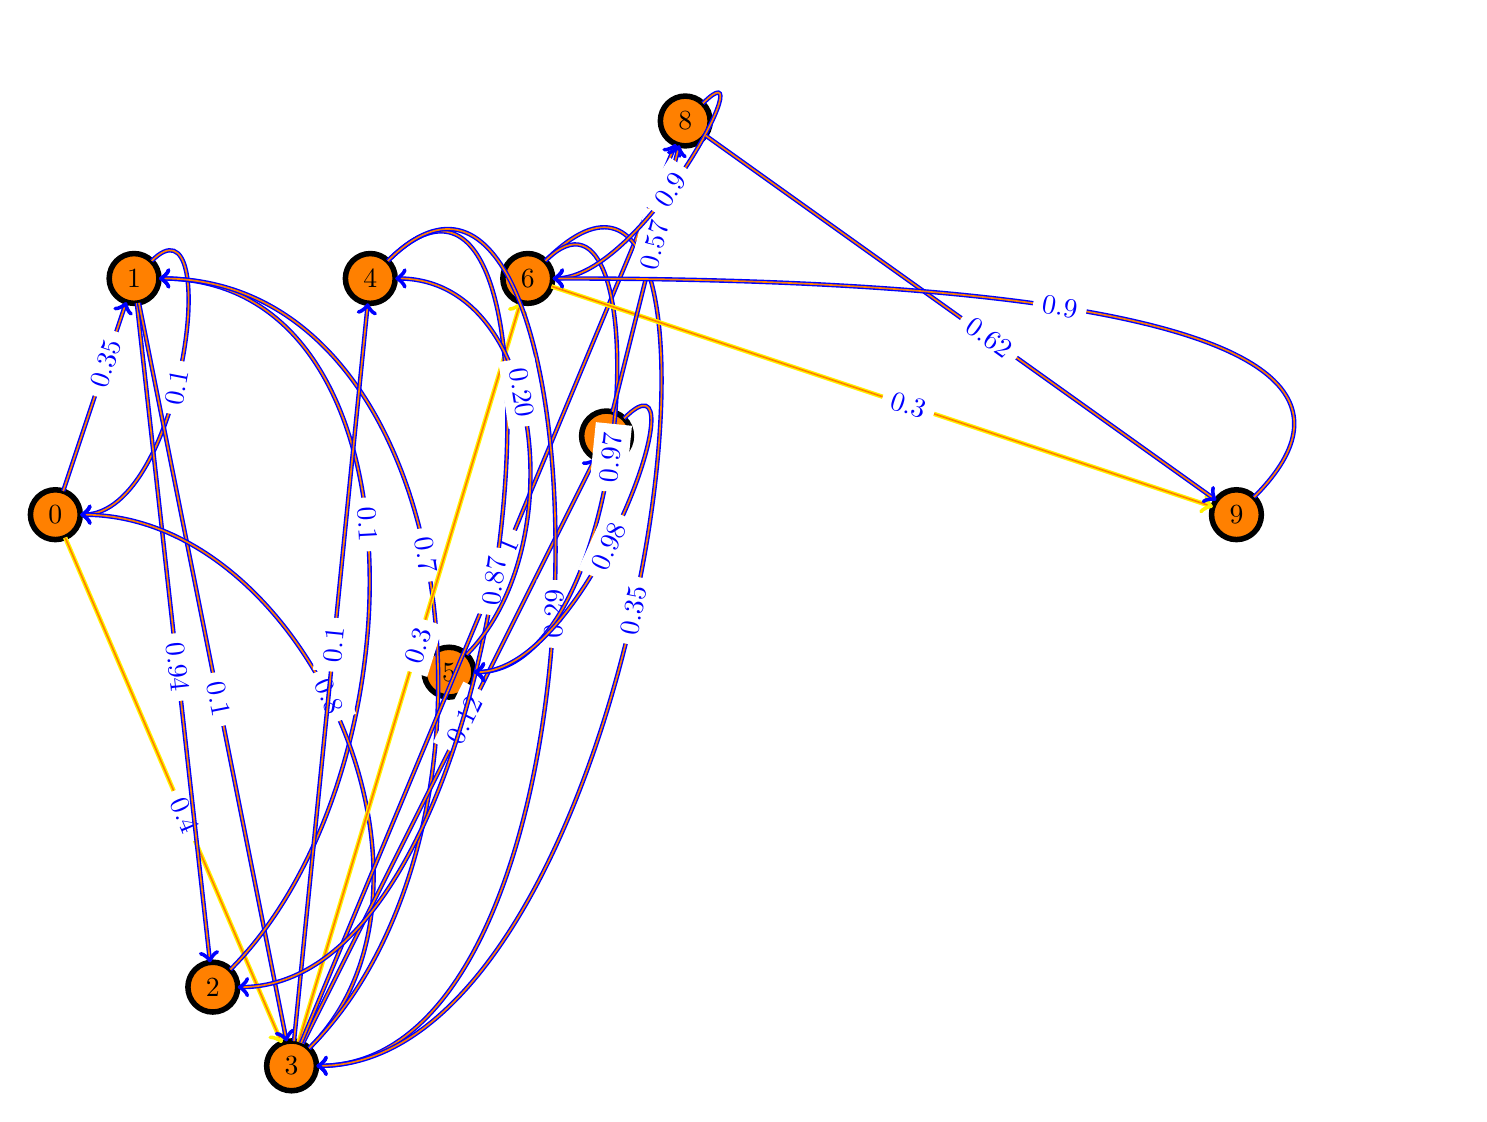
\begin{tikzpicture}
\SetVertexNormal[Shape      = circle,
FillColor  = orange,
LineWidth  = 2pt]
\SetUpEdge[lw         = 0.5pt,
color      = black,
labelcolor = white,
labeltext  = red,
labelstyle = {sloped,text=blue}]
\tikzstyle{TempStyle}=[double = orange]
\Vertex[x=-10, y=8]{0}
\Vertex[x=-9, y=11]{1}
\Vertex[x=-8, y=2]{2}
\Vertex[x=-7, y=1]{3}
\Vertex[x=-6, y=11]{4}
\Vertex[x=-5, y=6]{5}
\Vertex[x=-4, y=11]{6}
\Vertex[x=-3, y=9]{7}
\Vertex[x=-2, y=13]{8}
\Vertex[x=5, y=8]{9}
\tikzset{EdgeStyle/.style={->,TempStyle,relative=false,right=60,color=blue}}
\Edge[label=$0.35$](0)(1)
\tikzset{EdgeStyle/.style={->,TempStyle,relative=false,right=60,color=yellow}}
\Edge[label=$0.4$](0)(3)
\tikzset{EdgeStyle/.style={->,TempStyle,relative=false,left=60,color=blue,in=0,draw}}
\Edge[label=$0.1$](1)(0)
\tikzset{EdgeStyle/.style={->,TempStyle,relative=false,right=60,color=blue}}
\Edge[label=$0.94$](1)(2)
\tikzset{EdgeStyle/.style={->,TempStyle,relative=false,right=60,color=blue}}
\Edge[label=$0.1$](1)(3)
\tikzset{EdgeStyle/.style={->,TempStyle,relative=false,left=60,color=blue,in=0,draw}}
\Edge[label=$0.1$](2)(1)
\tikzset{EdgeStyle/.style={->,TempStyle,relative=false,left=60,color=blue,in=0,draw}}
\Edge[label=$0.8$](3)(0)
\tikzset{EdgeStyle/.style={->,TempStyle,relative=false,left=60,color=blue,in=0,draw}}
\Edge[label=$0.7$](3)(1)
\tikzset{EdgeStyle/.style={->,TempStyle,relative=false,right=60,color=blue}}
\Edge[label=$0.1$](3)(4)
\tikzset{EdgeStyle/.style={->,TempStyle,relative=false,right=60,color=yellow}}
\Edge[label=$0.3$](3)(6)
\tikzset{EdgeStyle/.style={->,TempStyle,relative=false,right=60,color=blue}}
\Edge[label=$0.12$](3)(7)
\tikzset{EdgeStyle/.style={->,TempStyle,relative=false,right=60,color=blue}}
\Edge[label=$0.61$](3)(8)
\tikzset{EdgeStyle/.style={->,TempStyle,relative=false,left=60,color=blue,in=0,draw}}
\Edge[label=$0.87$](4)(2)
\tikzset{EdgeStyle/.style={->,TempStyle,relative=false,left=60,color=blue,in=0,draw}}
\Edge[label=$0.29$](4)(3)
\tikzset{EdgeStyle/.style={->,TempStyle,relative=false,left=60,color=blue,in=0,draw}}
\Edge[label=$0.20$](5)(4)
\tikzset{EdgeStyle/.style={->,TempStyle,relative=false,left=60,color=blue,in=0,draw}}
\Edge[label=$0.35$](6)(3)
\tikzset{EdgeStyle/.style={->,TempStyle,relative=false,left=60,color=blue,in=0,draw}}
\Edge[label=$0.97$](6)(5)
\tikzset{EdgeStyle/.style={->,TempStyle,relative=false,right=60,color=yellow}}
\Edge[label=$0.3$](6)(9)
\tikzset{EdgeStyle/.style={->,TempStyle,relative=false,left=60,color=blue,in=0,draw}}
\Edge[label=$0.98$](7)(5)
\tikzset{EdgeStyle/.style={->,TempStyle,relative=false,right=60,color=blue}}
\Edge[label=$0.57$](7)(8)
\tikzset{EdgeStyle/.style={->,TempStyle,relative=false,left=60,color=blue,in=0,draw}}
\Edge[label=$0.9$](8)(6)
\tikzset{EdgeStyle/.style={->,TempStyle,relative=false,right=60,color=blue}}
\Edge[label=$0.62$](8)(9)
\tikzset{EdgeStyle/.style={->,TempStyle,relative=false,left=60,color=blue,in=0,draw}}
\Edge[label=$0.9$](9)(6)
\end{tikzpicture}\\
\begin{center}\begin{tabular}{l c}\\
\textcolor{orange}{\LARGE$\rightarrow$} & Chemin \\
 \textcolor{red}{\LARGE$\rightarrow$} & Créations arcs\\
 \textcolor{green}{\LARGE$\rightarrow$} & Modification flot\\
\end{tabular}
\end{center}
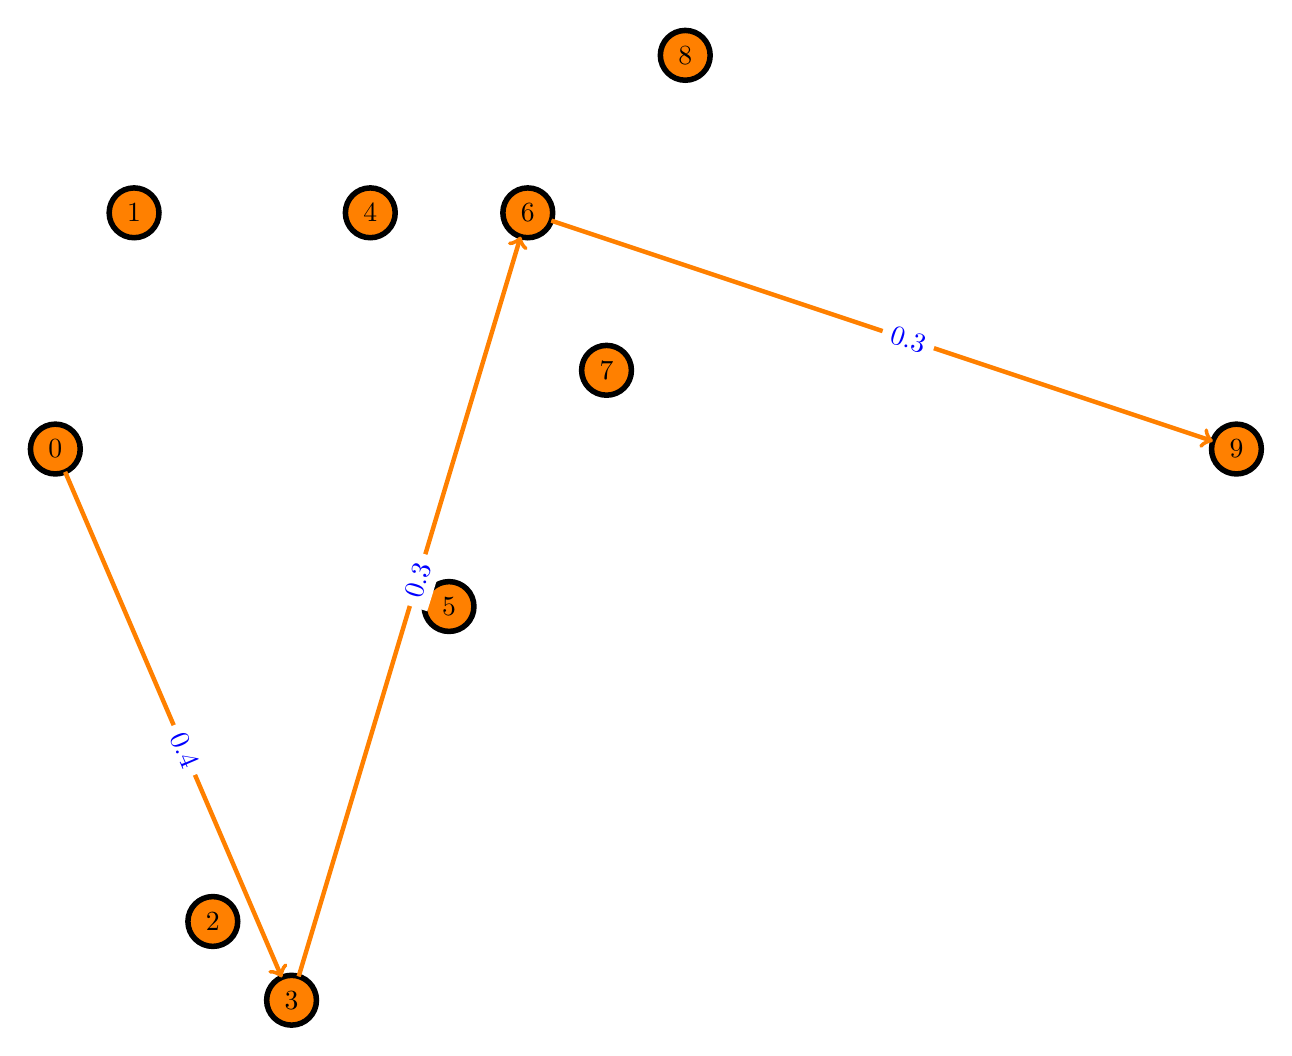
\begin{tikzpicture}
\SetVertexNormal[Shape      = circle,
FillColor  = orange,
LineWidth  = 2pt]
\SetUpEdge[lw         = 0.5pt,
color      = black,
labelcolor = white,
labeltext  = red,
labelstyle = {sloped,text=blue}]
\tikzstyle{TempStyle}=[double = orange]
\Vertex[x=-10, y=8]{0}
\Vertex[x=-9, y=11]{1}
\Vertex[x=-8, y=2]{2}
\Vertex[x=-7, y=1]{3}
\Vertex[x=-6, y=11]{4}
\Vertex[x=-5, y=6]{5}
\Vertex[x=-4, y=11]{6}
\Vertex[x=-3, y=9]{7}
\Vertex[x=-2, y=13]{8}
\Vertex[x=5, y=8]{9}
\tikzset{EdgeStyle/.style={->,TempStyle,relative=false,right=60,color=orange}}
\Edge[label=$0.4$](0)(3)
\tikzset{EdgeStyle/.style={->,TempStyle,relative=false,right=60,color=orange}}
\Edge[label=$0.3$](3)(6)
\tikzset{EdgeStyle/.style={->,TempStyle,relative=false,right=60,color=orange}}
\Edge[label=$0.3$](6)(9)
\end{tikzpicture}\\
\begin{center}\begin{tabular}{l c}\\
\textcolor{orange}{\LARGE$\rightarrow$} & Chemin \\
 \textcolor{red}{\LARGE$\rightarrow$} & Créations arcs\\
 \textcolor{green}{\LARGE$\rightarrow$} & Modification flot\\
\end{tabular}
\end{center}
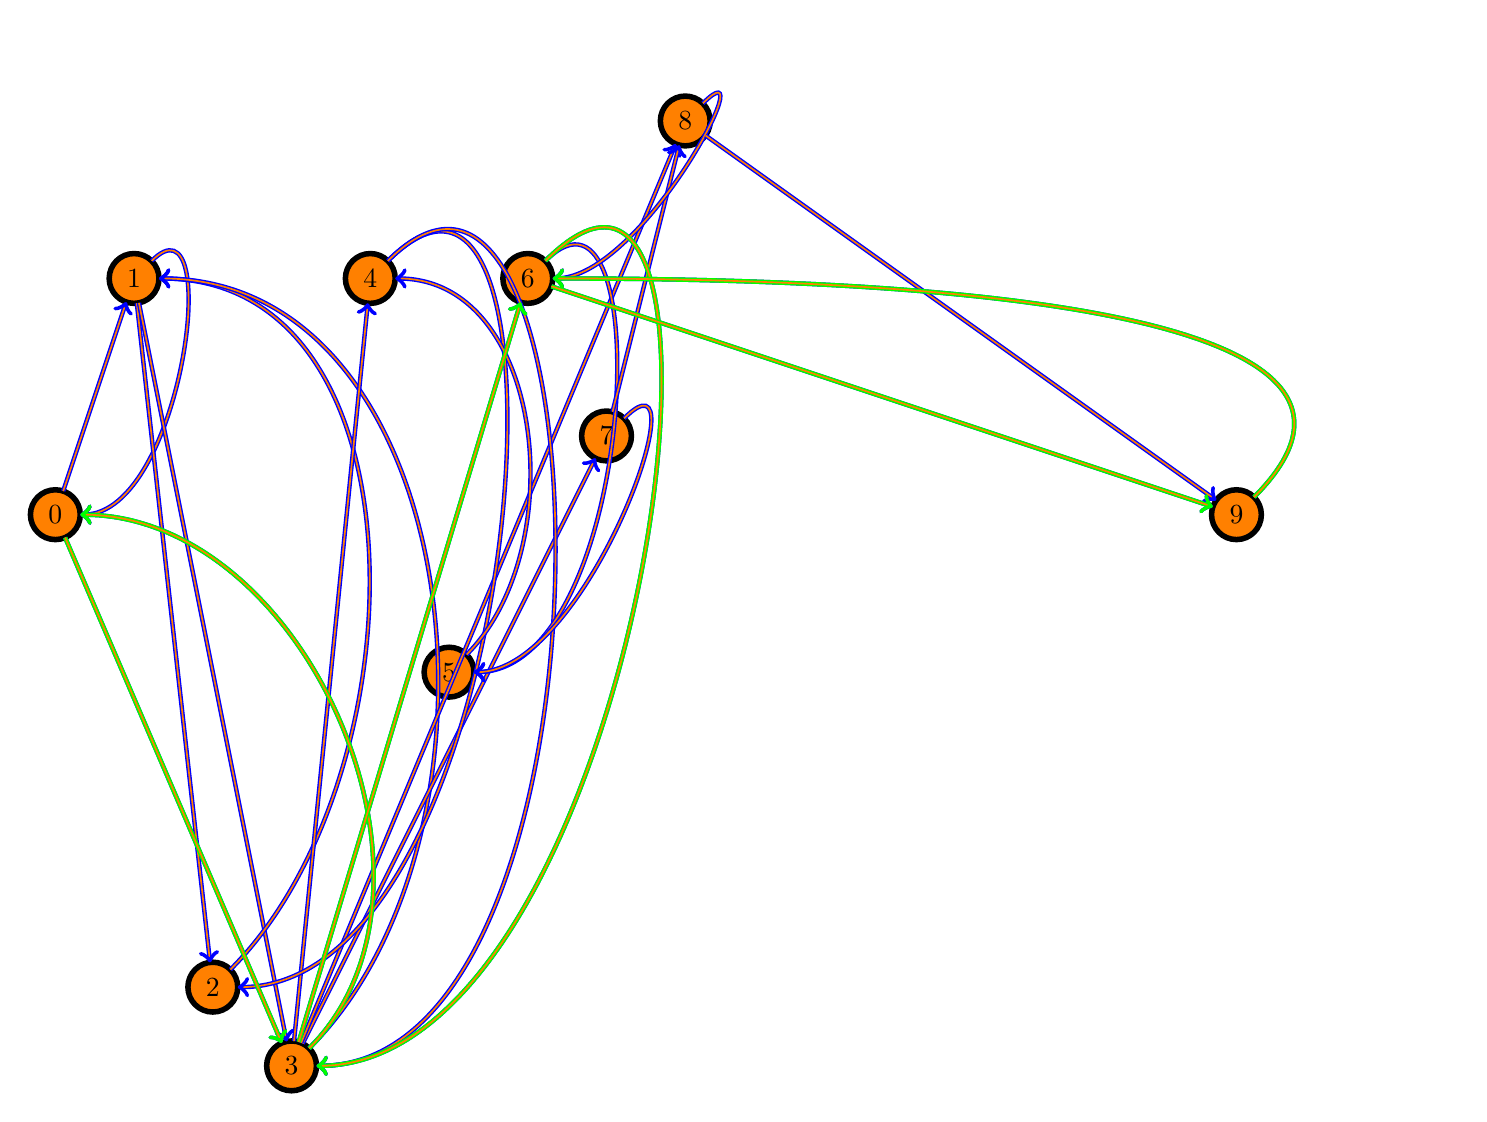
\begin{tikzpicture}
\SetVertexNormal[Shape      = circle,
FillColor  = orange,
LineWidth  = 2pt]
\SetUpEdge[lw         = 0.5pt,
color      = black,
labelcolor = white,
labeltext  = red,
labelstyle = {sloped,text=blue}]
\tikzstyle{TempStyle}=[double = orange]
\Vertex[x=-10, y=8]{0}
\Vertex[x=-9, y=11]{1}
\Vertex[x=-8, y=2]{2}
\Vertex[x=-7, y=1]{3}
\Vertex[x=-6, y=11]{4}
\Vertex[x=-5, y=6]{5}
\Vertex[x=-4, y=11]{6}
\Vertex[x=-3, y=9]{7}
\Vertex[x=-2, y=13]{8}
\Vertex[x=5, y=8]{9}
\tikzset{EdgeStyle/.style={->,TempStyle,relative=false,right=60,color=blue}}
\Edge(0)(1)
\tikzset{EdgeStyle/.style={->,TempStyle,relative=false,right=60,color=blue}}
\Edge(0)(3)
\tikzset{EdgeStyle/.style={->,TempStyle,relative=false,left=60,color=blue,in=0,draw}}
\Edge(1)(0)
\tikzset{EdgeStyle/.style={->,TempStyle,relative=false,right=60,color=blue}}
\Edge(1)(2)
\tikzset{EdgeStyle/.style={->,TempStyle,relative=false,right=60,color=blue}}
\Edge(1)(3)
\tikzset{EdgeStyle/.style={->,TempStyle,relative=false,left=60,color=blue,in=0,draw}}
\Edge(2)(1)
\tikzset{EdgeStyle/.style={->,TempStyle,relative=false,left=60,color=blue,in=0,draw}}
\Edge(3)(0)
\tikzset{EdgeStyle/.style={->,TempStyle,relative=false,left=60,color=blue,in=0,draw}}
\Edge(3)(1)
\tikzset{EdgeStyle/.style={->,TempStyle,relative=false,right=60,color=blue}}
\Edge(3)(4)
\tikzset{EdgeStyle/.style={->,TempStyle,relative=false,right=60,color=blue}}
\Edge(3)(6)
\tikzset{EdgeStyle/.style={->,TempStyle,relative=false,right=60,color=blue}}
\Edge(3)(7)
\tikzset{EdgeStyle/.style={->,TempStyle,relative=false,right=60,color=blue}}
\Edge(3)(8)
\tikzset{EdgeStyle/.style={->,TempStyle,relative=false,left=60,color=blue,in=0,draw}}
\Edge(4)(2)
\tikzset{EdgeStyle/.style={->,TempStyle,relative=false,left=60,color=blue,in=0,draw}}
\Edge(4)(3)
\tikzset{EdgeStyle/.style={->,TempStyle,relative=false,left=60,color=blue,in=0,draw}}
\Edge(5)(4)
\tikzset{EdgeStyle/.style={->,TempStyle,relative=false,left=60,color=blue,in=0,draw}}
\Edge(6)(3)
\tikzset{EdgeStyle/.style={->,TempStyle,relative=false,left=60,color=blue,in=0,draw}}
\Edge(6)(5)
\tikzset{EdgeStyle/.style={->,TempStyle,relative=false,right=60,color=blue}}
\Edge(6)(9)
\tikzset{EdgeStyle/.style={->,TempStyle,relative=false,left=60,color=blue,in=0,draw}}
\Edge(7)(5)
\tikzset{EdgeStyle/.style={->,TempStyle,relative=false,right=60,color=blue}}
\Edge(7)(8)
\tikzset{EdgeStyle/.style={->,TempStyle,relative=false,left=60,color=blue,in=0,draw}}
\Edge(8)(6)
\tikzset{EdgeStyle/.style={->,TempStyle,relative=false,right=60,color=blue}}
\Edge(8)(9)
\tikzset{EdgeStyle/.style={->,TempStyle,relative=false,left=60,color=blue,in=0,draw}}
\Edge(9)(6)
\tikzset{EdgeStyle/.style={->,TempStyle,relative=false,right=60,color=green}}
\Edge(0)(3)
\tikzset{EdgeStyle/.style={->,TempStyle,relative=false,right=60,in=0,color=green}}
\Edge(3)(0)
\tikzset{EdgeStyle/.style={->,TempStyle,relative=false,right=60,color=green}}
\Edge(3)(6)
\tikzset{EdgeStyle/.style={->,TempStyle,relative=false,right=60,in=0,color=green}}
\Edge(6)(3)
\tikzset{EdgeStyle/.style={->,TempStyle,relative=false,right=60,color=green}}
\Edge(6)(9)
\tikzset{EdgeStyle/.style={->,TempStyle,relative=false,right=60,in=0,color=green}}
\Edge(9)(6)
\end{tikzpicture}\\
\begin{center}\begin{tabular}{l c}\\
\textcolor{orange}{\LARGE$\rightarrow$} & Chemin \\
 \textcolor{red}{\LARGE$\rightarrow$} & Créations arcs\\
 \textcolor{green}{\LARGE$\rightarrow$} & Modification flot\\
\end{tabular}
\end{center}
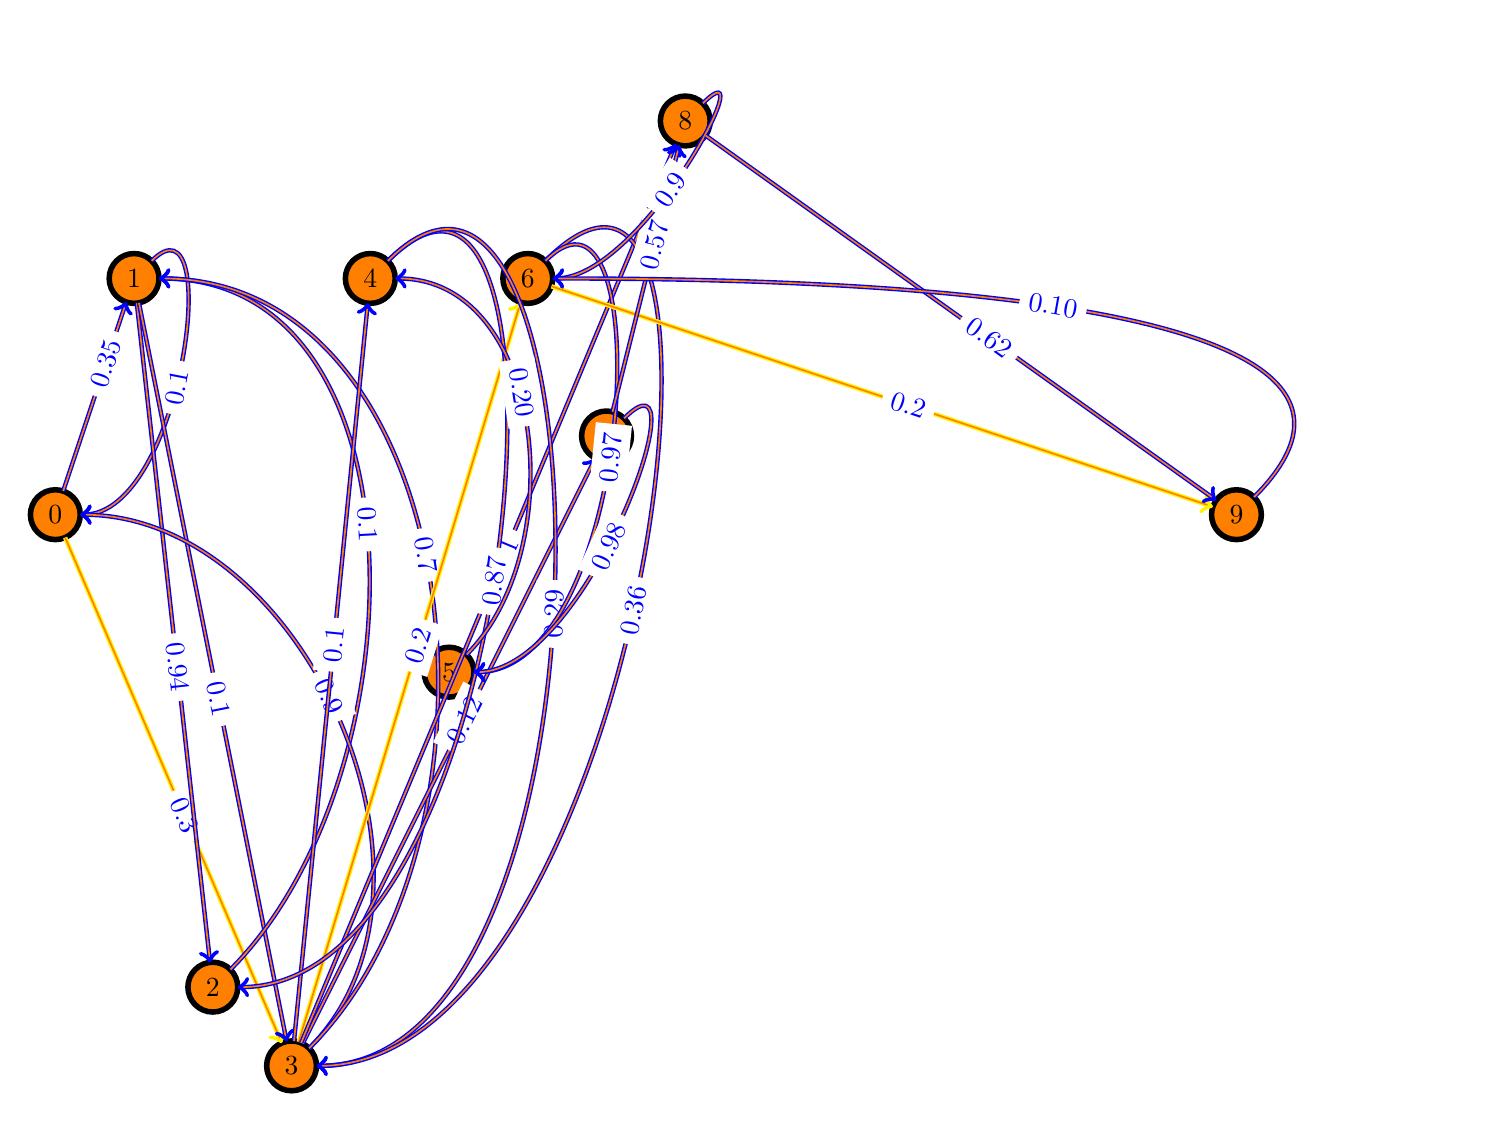
\begin{tikzpicture}
\SetVertexNormal[Shape      = circle,
FillColor  = orange,
LineWidth  = 2pt]
\SetUpEdge[lw         = 0.5pt,
color      = black,
labelcolor = white,
labeltext  = red,
labelstyle = {sloped,text=blue}]
\tikzstyle{TempStyle}=[double = orange]
\Vertex[x=-10, y=8]{0}
\Vertex[x=-9, y=11]{1}
\Vertex[x=-8, y=2]{2}
\Vertex[x=-7, y=1]{3}
\Vertex[x=-6, y=11]{4}
\Vertex[x=-5, y=6]{5}
\Vertex[x=-4, y=11]{6}
\Vertex[x=-3, y=9]{7}
\Vertex[x=-2, y=13]{8}
\Vertex[x=5, y=8]{9}
\tikzset{EdgeStyle/.style={->,TempStyle,relative=false,right=60,color=blue}}
\Edge[label=$0.35$](0)(1)
\tikzset{EdgeStyle/.style={->,TempStyle,relative=false,right=60,color=yellow}}
\Edge[label=$0.3$](0)(3)
\tikzset{EdgeStyle/.style={->,TempStyle,relative=false,left=60,color=blue,in=0,draw}}
\Edge[label=$0.1$](1)(0)
\tikzset{EdgeStyle/.style={->,TempStyle,relative=false,right=60,color=blue}}
\Edge[label=$0.94$](1)(2)
\tikzset{EdgeStyle/.style={->,TempStyle,relative=false,right=60,color=blue}}
\Edge[label=$0.1$](1)(3)
\tikzset{EdgeStyle/.style={->,TempStyle,relative=false,left=60,color=blue,in=0,draw}}
\Edge[label=$0.1$](2)(1)
\tikzset{EdgeStyle/.style={->,TempStyle,relative=false,left=60,color=blue,in=0,draw}}
\Edge[label=$0.9$](3)(0)
\tikzset{EdgeStyle/.style={->,TempStyle,relative=false,left=60,color=blue,in=0,draw}}
\Edge[label=$0.7$](3)(1)
\tikzset{EdgeStyle/.style={->,TempStyle,relative=false,right=60,color=blue}}
\Edge[label=$0.1$](3)(4)
\tikzset{EdgeStyle/.style={->,TempStyle,relative=false,right=60,color=yellow}}
\Edge[label=$0.2$](3)(6)
\tikzset{EdgeStyle/.style={->,TempStyle,relative=false,right=60,color=blue}}
\Edge[label=$0.12$](3)(7)
\tikzset{EdgeStyle/.style={->,TempStyle,relative=false,right=60,color=blue}}
\Edge[label=$0.61$](3)(8)
\tikzset{EdgeStyle/.style={->,TempStyle,relative=false,left=60,color=blue,in=0,draw}}
\Edge[label=$0.87$](4)(2)
\tikzset{EdgeStyle/.style={->,TempStyle,relative=false,left=60,color=blue,in=0,draw}}
\Edge[label=$0.29$](4)(3)
\tikzset{EdgeStyle/.style={->,TempStyle,relative=false,left=60,color=blue,in=0,draw}}
\Edge[label=$0.20$](5)(4)
\tikzset{EdgeStyle/.style={->,TempStyle,relative=false,left=60,color=blue,in=0,draw}}
\Edge[label=$0.36$](6)(3)
\tikzset{EdgeStyle/.style={->,TempStyle,relative=false,left=60,color=blue,in=0,draw}}
\Edge[label=$0.97$](6)(5)
\tikzset{EdgeStyle/.style={->,TempStyle,relative=false,right=60,color=yellow}}
\Edge[label=$0.2$](6)(9)
\tikzset{EdgeStyle/.style={->,TempStyle,relative=false,left=60,color=blue,in=0,draw}}
\Edge[label=$0.98$](7)(5)
\tikzset{EdgeStyle/.style={->,TempStyle,relative=false,right=60,color=blue}}
\Edge[label=$0.57$](7)(8)
\tikzset{EdgeStyle/.style={->,TempStyle,relative=false,left=60,color=blue,in=0,draw}}
\Edge[label=$0.9$](8)(6)
\tikzset{EdgeStyle/.style={->,TempStyle,relative=false,right=60,color=blue}}
\Edge[label=$0.62$](8)(9)
\tikzset{EdgeStyle/.style={->,TempStyle,relative=false,left=60,color=blue,in=0,draw}}
\Edge[label=$0.10$](9)(6)
\end{tikzpicture}\\
\begin{center}\begin{tabular}{l c}\\
\textcolor{orange}{\LARGE$\rightarrow$} & Chemin \\
 \textcolor{red}{\LARGE$\rightarrow$} & Créations arcs\\
 \textcolor{green}{\LARGE$\rightarrow$} & Modification flot\\
\end{tabular}
\end{center}
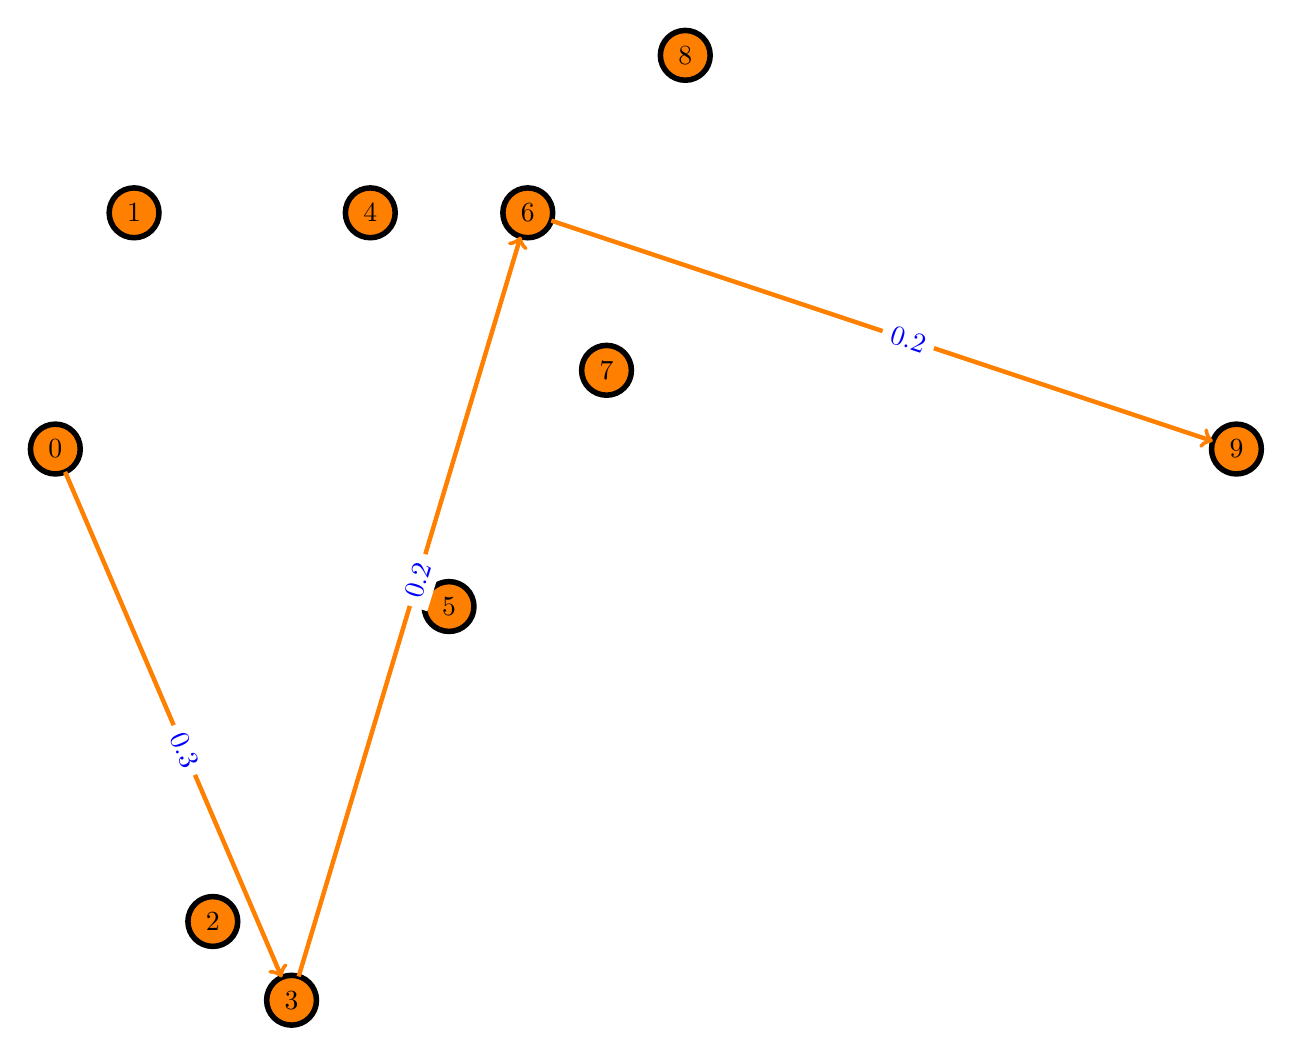
\begin{tikzpicture}
\SetVertexNormal[Shape      = circle,
FillColor  = orange,
LineWidth  = 2pt]
\SetUpEdge[lw         = 0.5pt,
color      = black,
labelcolor = white,
labeltext  = red,
labelstyle = {sloped,text=blue}]
\tikzstyle{TempStyle}=[double = orange]
\Vertex[x=-10, y=8]{0}
\Vertex[x=-9, y=11]{1}
\Vertex[x=-8, y=2]{2}
\Vertex[x=-7, y=1]{3}
\Vertex[x=-6, y=11]{4}
\Vertex[x=-5, y=6]{5}
\Vertex[x=-4, y=11]{6}
\Vertex[x=-3, y=9]{7}
\Vertex[x=-2, y=13]{8}
\Vertex[x=5, y=8]{9}
\tikzset{EdgeStyle/.style={->,TempStyle,relative=false,right=60,color=orange}}
\Edge[label=$0.3$](0)(3)
\tikzset{EdgeStyle/.style={->,TempStyle,relative=false,right=60,color=orange}}
\Edge[label=$0.2$](3)(6)
\tikzset{EdgeStyle/.style={->,TempStyle,relative=false,right=60,color=orange}}
\Edge[label=$0.2$](6)(9)
\end{tikzpicture}\\
\begin{center}\begin{tabular}{l c}\\
\textcolor{orange}{\LARGE$\rightarrow$} & Chemin \\
 \textcolor{red}{\LARGE$\rightarrow$} & Créations arcs\\
 \textcolor{green}{\LARGE$\rightarrow$} & Modification flot\\
\end{tabular}
\end{center}
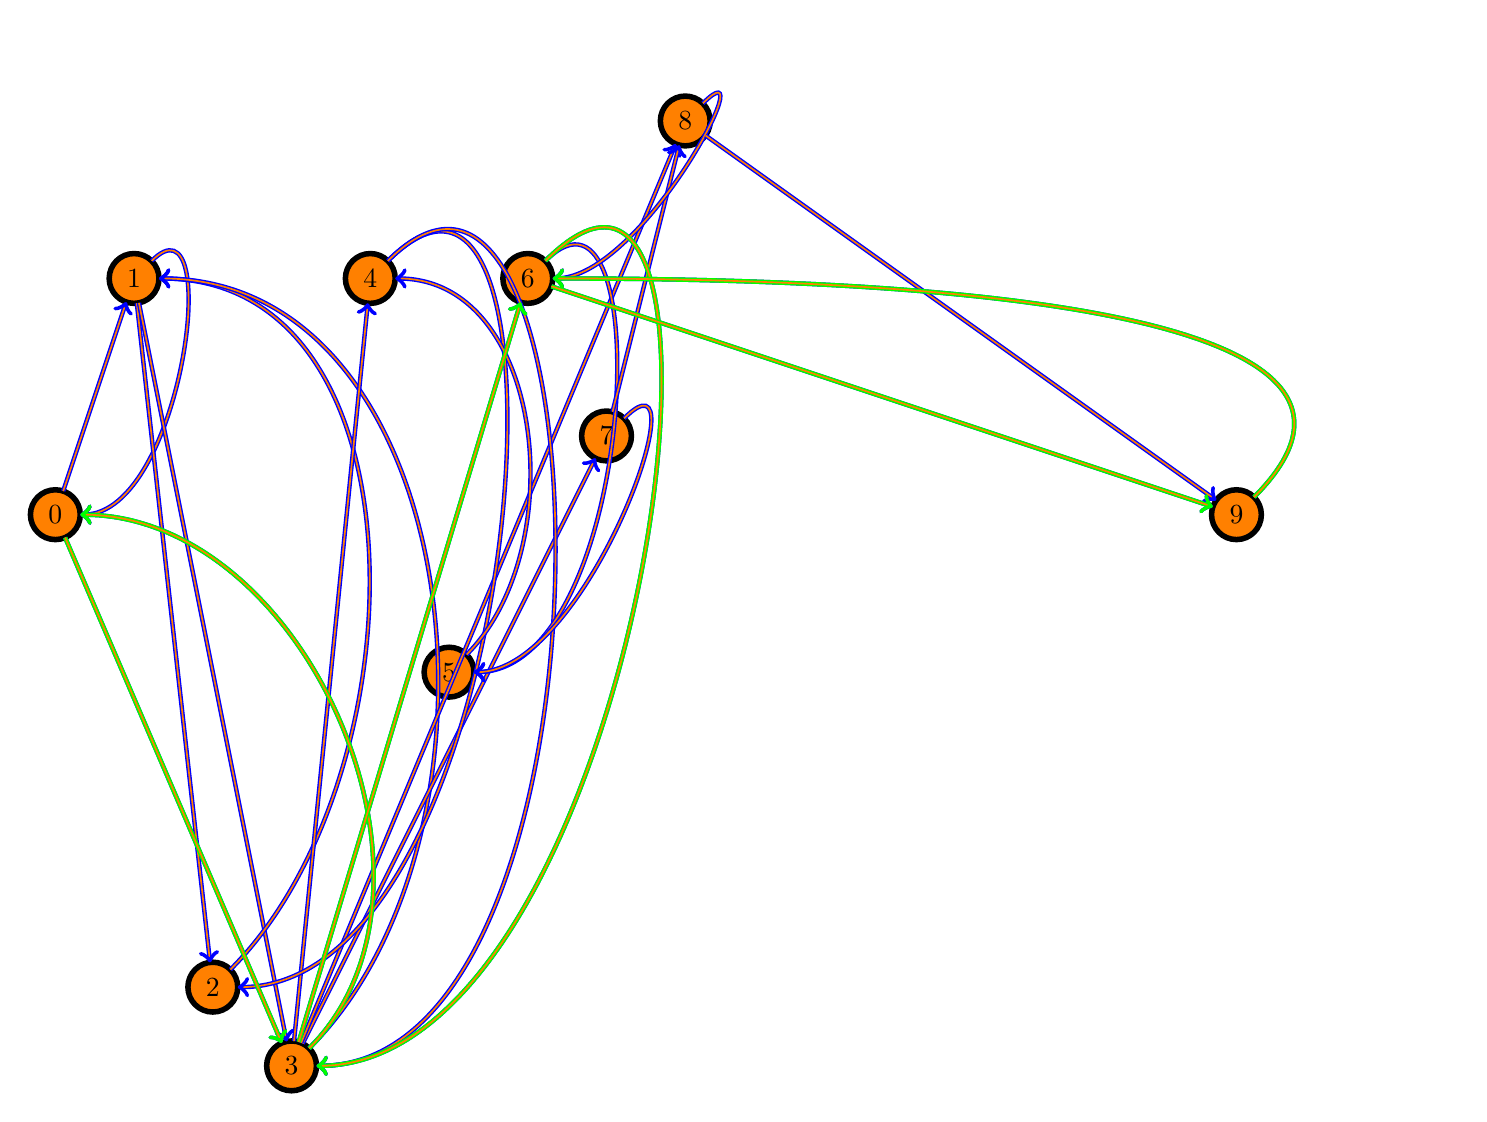
\begin{tikzpicture}
\SetVertexNormal[Shape      = circle,
FillColor  = orange,
LineWidth  = 2pt]
\SetUpEdge[lw         = 0.5pt,
color      = black,
labelcolor = white,
labeltext  = red,
labelstyle = {sloped,text=blue}]
\tikzstyle{TempStyle}=[double = orange]
\Vertex[x=-10, y=8]{0}
\Vertex[x=-9, y=11]{1}
\Vertex[x=-8, y=2]{2}
\Vertex[x=-7, y=1]{3}
\Vertex[x=-6, y=11]{4}
\Vertex[x=-5, y=6]{5}
\Vertex[x=-4, y=11]{6}
\Vertex[x=-3, y=9]{7}
\Vertex[x=-2, y=13]{8}
\Vertex[x=5, y=8]{9}
\tikzset{EdgeStyle/.style={->,TempStyle,relative=false,right=60,color=blue}}
\Edge(0)(1)
\tikzset{EdgeStyle/.style={->,TempStyle,relative=false,right=60,color=blue}}
\Edge(0)(3)
\tikzset{EdgeStyle/.style={->,TempStyle,relative=false,left=60,color=blue,in=0,draw}}
\Edge(1)(0)
\tikzset{EdgeStyle/.style={->,TempStyle,relative=false,right=60,color=blue}}
\Edge(1)(2)
\tikzset{EdgeStyle/.style={->,TempStyle,relative=false,right=60,color=blue}}
\Edge(1)(3)
\tikzset{EdgeStyle/.style={->,TempStyle,relative=false,left=60,color=blue,in=0,draw}}
\Edge(2)(1)
\tikzset{EdgeStyle/.style={->,TempStyle,relative=false,left=60,color=blue,in=0,draw}}
\Edge(3)(0)
\tikzset{EdgeStyle/.style={->,TempStyle,relative=false,left=60,color=blue,in=0,draw}}
\Edge(3)(1)
\tikzset{EdgeStyle/.style={->,TempStyle,relative=false,right=60,color=blue}}
\Edge(3)(4)
\tikzset{EdgeStyle/.style={->,TempStyle,relative=false,right=60,color=blue}}
\Edge(3)(6)
\tikzset{EdgeStyle/.style={->,TempStyle,relative=false,right=60,color=blue}}
\Edge(3)(7)
\tikzset{EdgeStyle/.style={->,TempStyle,relative=false,right=60,color=blue}}
\Edge(3)(8)
\tikzset{EdgeStyle/.style={->,TempStyle,relative=false,left=60,color=blue,in=0,draw}}
\Edge(4)(2)
\tikzset{EdgeStyle/.style={->,TempStyle,relative=false,left=60,color=blue,in=0,draw}}
\Edge(4)(3)
\tikzset{EdgeStyle/.style={->,TempStyle,relative=false,left=60,color=blue,in=0,draw}}
\Edge(5)(4)
\tikzset{EdgeStyle/.style={->,TempStyle,relative=false,left=60,color=blue,in=0,draw}}
\Edge(6)(3)
\tikzset{EdgeStyle/.style={->,TempStyle,relative=false,left=60,color=blue,in=0,draw}}
\Edge(6)(5)
\tikzset{EdgeStyle/.style={->,TempStyle,relative=false,right=60,color=blue}}
\Edge(6)(9)
\tikzset{EdgeStyle/.style={->,TempStyle,relative=false,left=60,color=blue,in=0,draw}}
\Edge(7)(5)
\tikzset{EdgeStyle/.style={->,TempStyle,relative=false,right=60,color=blue}}
\Edge(7)(8)
\tikzset{EdgeStyle/.style={->,TempStyle,relative=false,left=60,color=blue,in=0,draw}}
\Edge(8)(6)
\tikzset{EdgeStyle/.style={->,TempStyle,relative=false,right=60,color=blue}}
\Edge(8)(9)
\tikzset{EdgeStyle/.style={->,TempStyle,relative=false,left=60,color=blue,in=0,draw}}
\Edge(9)(6)
\tikzset{EdgeStyle/.style={->,TempStyle,relative=false,right=60,color=green}}
\Edge(0)(3)
\tikzset{EdgeStyle/.style={->,TempStyle,relative=false,right=60,in=0,color=green}}
\Edge(3)(0)
\tikzset{EdgeStyle/.style={->,TempStyle,relative=false,right=60,color=green}}
\Edge(3)(6)
\tikzset{EdgeStyle/.style={->,TempStyle,relative=false,right=60,in=0,color=green}}
\Edge(6)(3)
\tikzset{EdgeStyle/.style={->,TempStyle,relative=false,right=60,color=green}}
\Edge(6)(9)
\tikzset{EdgeStyle/.style={->,TempStyle,relative=false,right=60,in=0,color=green}}
\Edge(9)(6)
\end{tikzpicture}\\
\begin{center}\begin{tabular}{l c}\\
\textcolor{orange}{\LARGE$\rightarrow$} & Chemin \\
 \textcolor{red}{\LARGE$\rightarrow$} & Créations arcs\\
 \textcolor{green}{\LARGE$\rightarrow$} & Modification flot\\
\end{tabular}
\end{center}
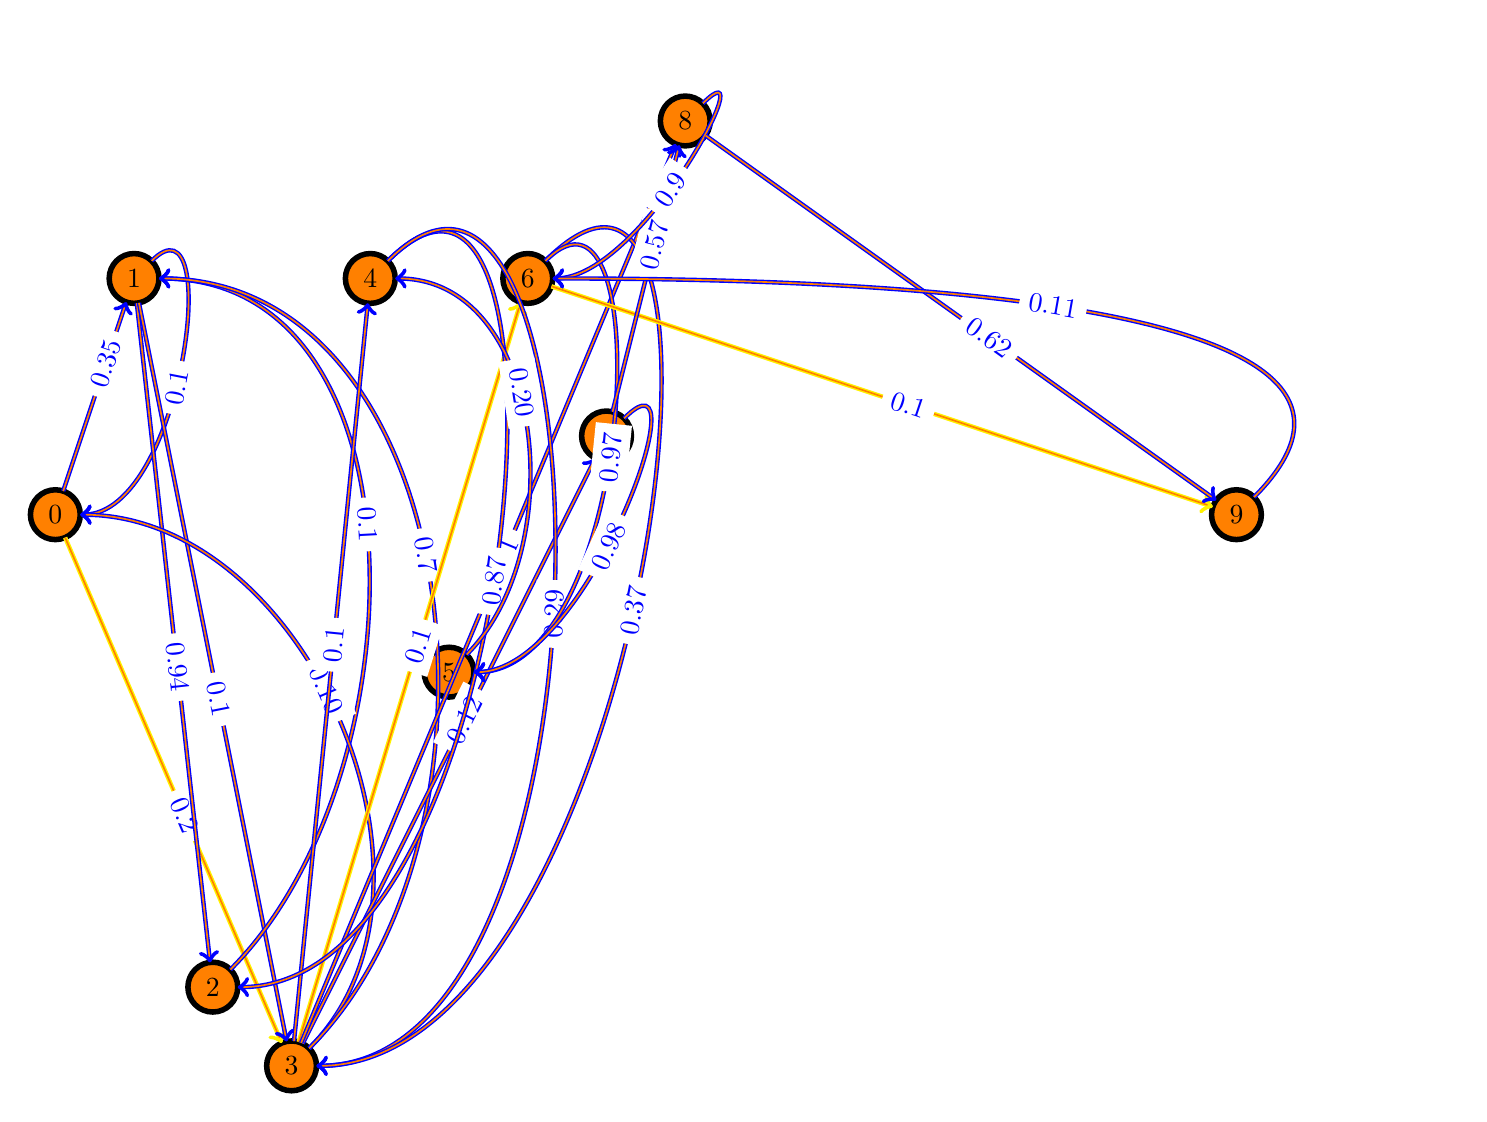
\begin{tikzpicture}
\SetVertexNormal[Shape      = circle,
FillColor  = orange,
LineWidth  = 2pt]
\SetUpEdge[lw         = 0.5pt,
color      = black,
labelcolor = white,
labeltext  = red,
labelstyle = {sloped,text=blue}]
\tikzstyle{TempStyle}=[double = orange]
\Vertex[x=-10, y=8]{0}
\Vertex[x=-9, y=11]{1}
\Vertex[x=-8, y=2]{2}
\Vertex[x=-7, y=1]{3}
\Vertex[x=-6, y=11]{4}
\Vertex[x=-5, y=6]{5}
\Vertex[x=-4, y=11]{6}
\Vertex[x=-3, y=9]{7}
\Vertex[x=-2, y=13]{8}
\Vertex[x=5, y=8]{9}
\tikzset{EdgeStyle/.style={->,TempStyle,relative=false,right=60,color=blue}}
\Edge[label=$0.35$](0)(1)
\tikzset{EdgeStyle/.style={->,TempStyle,relative=false,right=60,color=yellow}}
\Edge[label=$0.2$](0)(3)
\tikzset{EdgeStyle/.style={->,TempStyle,relative=false,left=60,color=blue,in=0,draw}}
\Edge[label=$0.1$](1)(0)
\tikzset{EdgeStyle/.style={->,TempStyle,relative=false,right=60,color=blue}}
\Edge[label=$0.94$](1)(2)
\tikzset{EdgeStyle/.style={->,TempStyle,relative=false,right=60,color=blue}}
\Edge[label=$0.1$](1)(3)
\tikzset{EdgeStyle/.style={->,TempStyle,relative=false,left=60,color=blue,in=0,draw}}
\Edge[label=$0.1$](2)(1)
\tikzset{EdgeStyle/.style={->,TempStyle,relative=false,left=60,color=blue,in=0,draw}}
\Edge[label=$0.10$](3)(0)
\tikzset{EdgeStyle/.style={->,TempStyle,relative=false,left=60,color=blue,in=0,draw}}
\Edge[label=$0.7$](3)(1)
\tikzset{EdgeStyle/.style={->,TempStyle,relative=false,right=60,color=blue}}
\Edge[label=$0.1$](3)(4)
\tikzset{EdgeStyle/.style={->,TempStyle,relative=false,right=60,color=yellow}}
\Edge[label=$0.1$](3)(6)
\tikzset{EdgeStyle/.style={->,TempStyle,relative=false,right=60,color=blue}}
\Edge[label=$0.12$](3)(7)
\tikzset{EdgeStyle/.style={->,TempStyle,relative=false,right=60,color=blue}}
\Edge[label=$0.61$](3)(8)
\tikzset{EdgeStyle/.style={->,TempStyle,relative=false,left=60,color=blue,in=0,draw}}
\Edge[label=$0.87$](4)(2)
\tikzset{EdgeStyle/.style={->,TempStyle,relative=false,left=60,color=blue,in=0,draw}}
\Edge[label=$0.29$](4)(3)
\tikzset{EdgeStyle/.style={->,TempStyle,relative=false,left=60,color=blue,in=0,draw}}
\Edge[label=$0.20$](5)(4)
\tikzset{EdgeStyle/.style={->,TempStyle,relative=false,left=60,color=blue,in=0,draw}}
\Edge[label=$0.37$](6)(3)
\tikzset{EdgeStyle/.style={->,TempStyle,relative=false,left=60,color=blue,in=0,draw}}
\Edge[label=$0.97$](6)(5)
\tikzset{EdgeStyle/.style={->,TempStyle,relative=false,right=60,color=yellow}}
\Edge[label=$0.1$](6)(9)
\tikzset{EdgeStyle/.style={->,TempStyle,relative=false,left=60,color=blue,in=0,draw}}
\Edge[label=$0.98$](7)(5)
\tikzset{EdgeStyle/.style={->,TempStyle,relative=false,right=60,color=blue}}
\Edge[label=$0.57$](7)(8)
\tikzset{EdgeStyle/.style={->,TempStyle,relative=false,left=60,color=blue,in=0,draw}}
\Edge[label=$0.9$](8)(6)
\tikzset{EdgeStyle/.style={->,TempStyle,relative=false,right=60,color=blue}}
\Edge[label=$0.62$](8)(9)
\tikzset{EdgeStyle/.style={->,TempStyle,relative=false,left=60,color=blue,in=0,draw}}
\Edge[label=$0.11$](9)(6)
\end{tikzpicture}\\
\begin{center}\begin{tabular}{l c}\\
\textcolor{orange}{\LARGE$\rightarrow$} & Chemin \\
 \textcolor{red}{\LARGE$\rightarrow$} & Créations arcs\\
 \textcolor{green}{\LARGE$\rightarrow$} & Modification flot\\
\end{tabular}
\end{center}
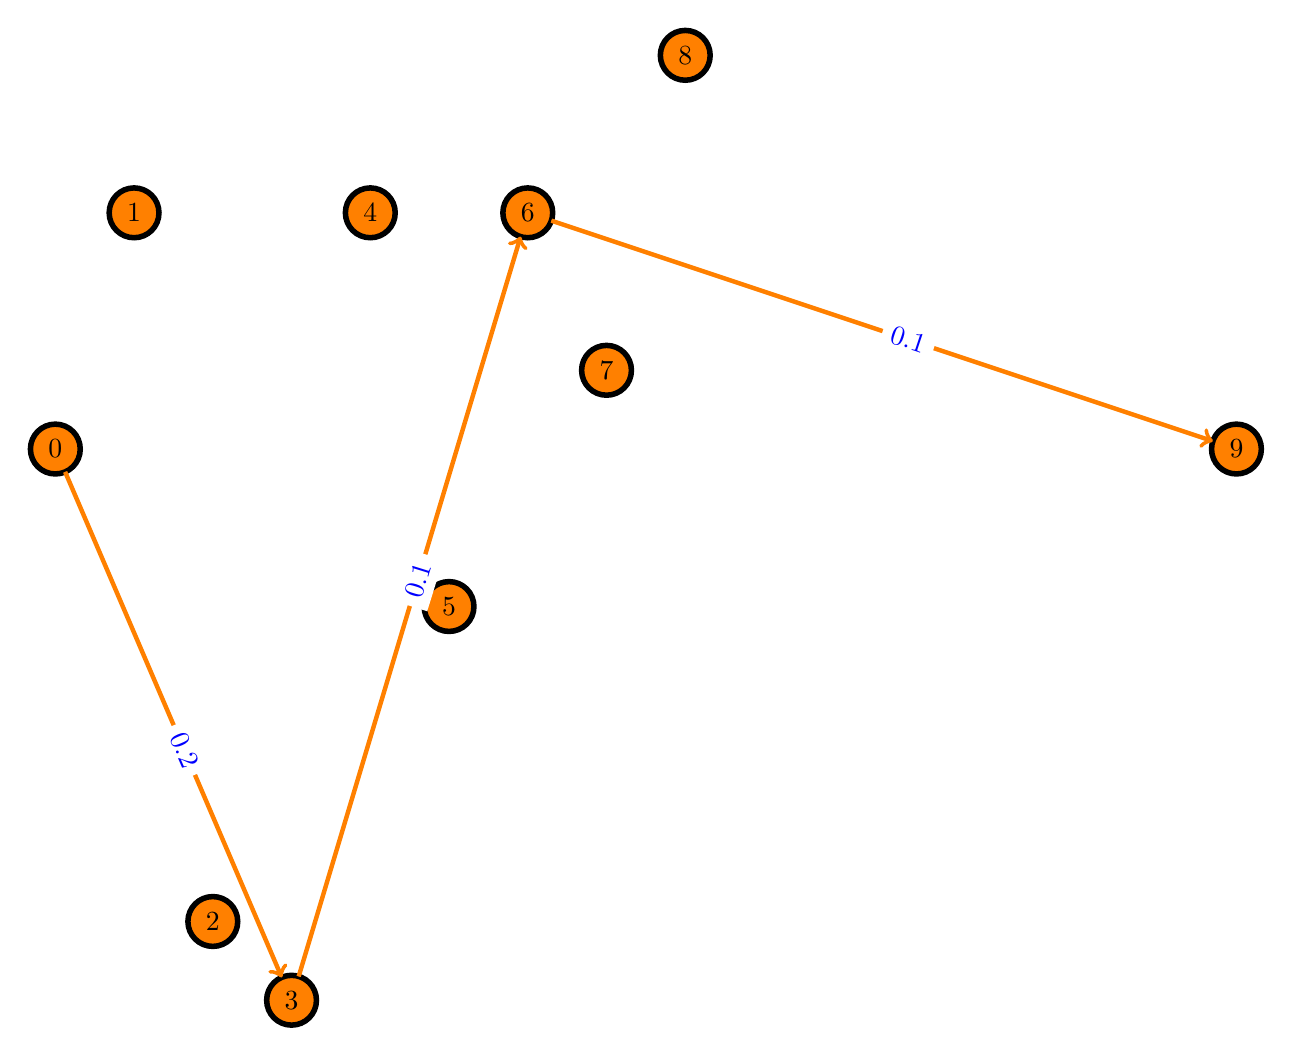
\begin{tikzpicture}
\SetVertexNormal[Shape      = circle,
FillColor  = orange,
LineWidth  = 2pt]
\SetUpEdge[lw         = 0.5pt,
color      = black,
labelcolor = white,
labeltext  = red,
labelstyle = {sloped,text=blue}]
\tikzstyle{TempStyle}=[double = orange]
\Vertex[x=-10, y=8]{0}
\Vertex[x=-9, y=11]{1}
\Vertex[x=-8, y=2]{2}
\Vertex[x=-7, y=1]{3}
\Vertex[x=-6, y=11]{4}
\Vertex[x=-5, y=6]{5}
\Vertex[x=-4, y=11]{6}
\Vertex[x=-3, y=9]{7}
\Vertex[x=-2, y=13]{8}
\Vertex[x=5, y=8]{9}
\tikzset{EdgeStyle/.style={->,TempStyle,relative=false,right=60,color=orange}}
\Edge[label=$0.2$](0)(3)
\tikzset{EdgeStyle/.style={->,TempStyle,relative=false,right=60,color=orange}}
\Edge[label=$0.1$](3)(6)
\tikzset{EdgeStyle/.style={->,TempStyle,relative=false,right=60,color=orange}}
\Edge[label=$0.1$](6)(9)
\end{tikzpicture}\\
\begin{center}\begin{tabular}{l c}\\
\textcolor{orange}{\LARGE$\rightarrow$} & Chemin \\
 \textcolor{red}{\LARGE$\rightarrow$} & Créations arcs\\
 \textcolor{green}{\LARGE$\rightarrow$} & Modification flot\\
\end{tabular}
\end{center}
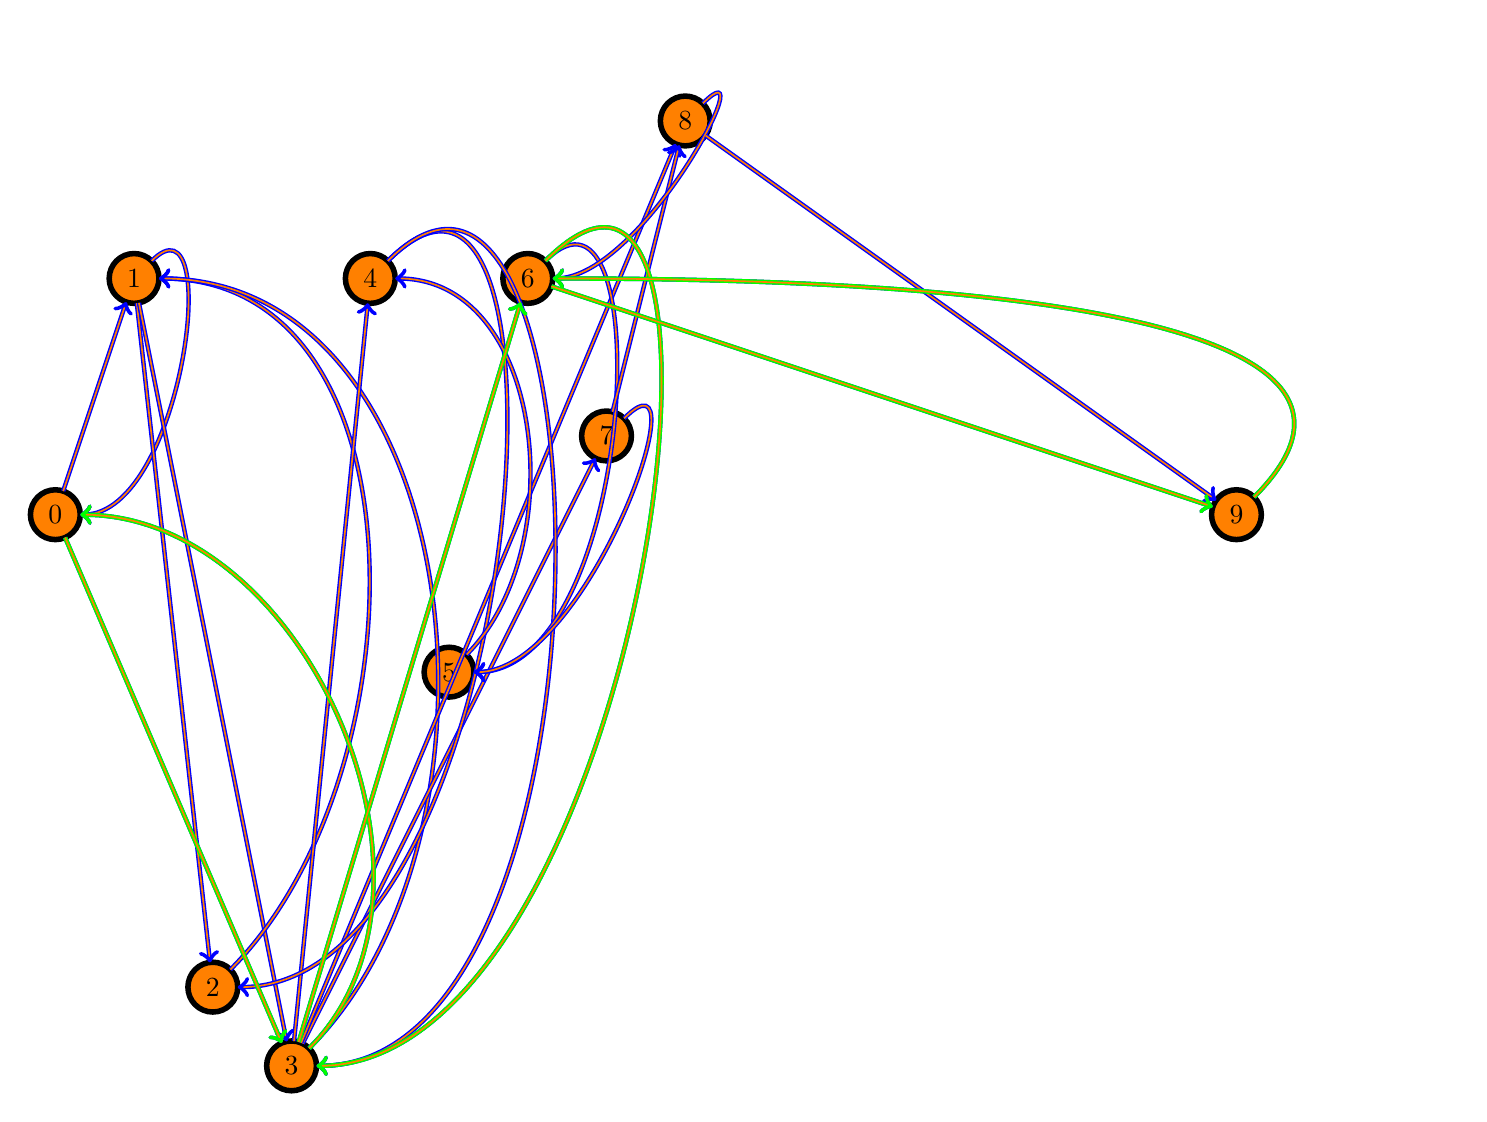
\begin{tikzpicture}
\SetVertexNormal[Shape      = circle,
FillColor  = orange,
LineWidth  = 2pt]
\SetUpEdge[lw         = 0.5pt,
color      = black,
labelcolor = white,
labeltext  = red,
labelstyle = {sloped,text=blue}]
\tikzstyle{TempStyle}=[double = orange]
\Vertex[x=-10, y=8]{0}
\Vertex[x=-9, y=11]{1}
\Vertex[x=-8, y=2]{2}
\Vertex[x=-7, y=1]{3}
\Vertex[x=-6, y=11]{4}
\Vertex[x=-5, y=6]{5}
\Vertex[x=-4, y=11]{6}
\Vertex[x=-3, y=9]{7}
\Vertex[x=-2, y=13]{8}
\Vertex[x=5, y=8]{9}
\tikzset{EdgeStyle/.style={->,TempStyle,relative=false,right=60,color=blue}}
\Edge(0)(1)
\tikzset{EdgeStyle/.style={->,TempStyle,relative=false,right=60,color=blue}}
\Edge(0)(3)
\tikzset{EdgeStyle/.style={->,TempStyle,relative=false,left=60,color=blue,in=0,draw}}
\Edge(1)(0)
\tikzset{EdgeStyle/.style={->,TempStyle,relative=false,right=60,color=blue}}
\Edge(1)(2)
\tikzset{EdgeStyle/.style={->,TempStyle,relative=false,right=60,color=blue}}
\Edge(1)(3)
\tikzset{EdgeStyle/.style={->,TempStyle,relative=false,left=60,color=blue,in=0,draw}}
\Edge(2)(1)
\tikzset{EdgeStyle/.style={->,TempStyle,relative=false,left=60,color=blue,in=0,draw}}
\Edge(3)(0)
\tikzset{EdgeStyle/.style={->,TempStyle,relative=false,left=60,color=blue,in=0,draw}}
\Edge(3)(1)
\tikzset{EdgeStyle/.style={->,TempStyle,relative=false,right=60,color=blue}}
\Edge(3)(4)
\tikzset{EdgeStyle/.style={->,TempStyle,relative=false,right=60,color=blue}}
\Edge(3)(6)
\tikzset{EdgeStyle/.style={->,TempStyle,relative=false,right=60,color=blue}}
\Edge(3)(7)
\tikzset{EdgeStyle/.style={->,TempStyle,relative=false,right=60,color=blue}}
\Edge(3)(8)
\tikzset{EdgeStyle/.style={->,TempStyle,relative=false,left=60,color=blue,in=0,draw}}
\Edge(4)(2)
\tikzset{EdgeStyle/.style={->,TempStyle,relative=false,left=60,color=blue,in=0,draw}}
\Edge(4)(3)
\tikzset{EdgeStyle/.style={->,TempStyle,relative=false,left=60,color=blue,in=0,draw}}
\Edge(5)(4)
\tikzset{EdgeStyle/.style={->,TempStyle,relative=false,left=60,color=blue,in=0,draw}}
\Edge(6)(3)
\tikzset{EdgeStyle/.style={->,TempStyle,relative=false,left=60,color=blue,in=0,draw}}
\Edge(6)(5)
\tikzset{EdgeStyle/.style={->,TempStyle,relative=false,right=60,color=blue}}
\Edge(6)(9)
\tikzset{EdgeStyle/.style={->,TempStyle,relative=false,left=60,color=blue,in=0,draw}}
\Edge(7)(5)
\tikzset{EdgeStyle/.style={->,TempStyle,relative=false,right=60,color=blue}}
\Edge(7)(8)
\tikzset{EdgeStyle/.style={->,TempStyle,relative=false,left=60,color=blue,in=0,draw}}
\Edge(8)(6)
\tikzset{EdgeStyle/.style={->,TempStyle,relative=false,right=60,color=blue}}
\Edge(8)(9)
\tikzset{EdgeStyle/.style={->,TempStyle,relative=false,left=60,color=blue,in=0,draw}}
\Edge(9)(6)
\tikzset{EdgeStyle/.style={->,TempStyle,relative=false,right=60,color=green}}
\Edge(0)(3)
\tikzset{EdgeStyle/.style={->,TempStyle,relative=false,right=60,in=0,color=green}}
\Edge(3)(0)
\tikzset{EdgeStyle/.style={->,TempStyle,relative=false,right=60,color=green}}
\Edge(3)(6)
\tikzset{EdgeStyle/.style={->,TempStyle,relative=false,right=60,in=0,color=green}}
\Edge(6)(3)
\tikzset{EdgeStyle/.style={->,TempStyle,relative=false,right=60,color=green}}
\Edge(6)(9)
\tikzset{EdgeStyle/.style={->,TempStyle,relative=false,right=60,in=0,color=green}}
\Edge(9)(6)
\end{tikzpicture}\\
\begin{center}\begin{tabular}{l c}\\
\textcolor{orange}{\LARGE$\rightarrow$} & Chemin \\
 \textcolor{red}{\LARGE$\rightarrow$} & Créations arcs\\
 \textcolor{green}{\LARGE$\rightarrow$} & Modification flot\\
\end{tabular}
\end{center}
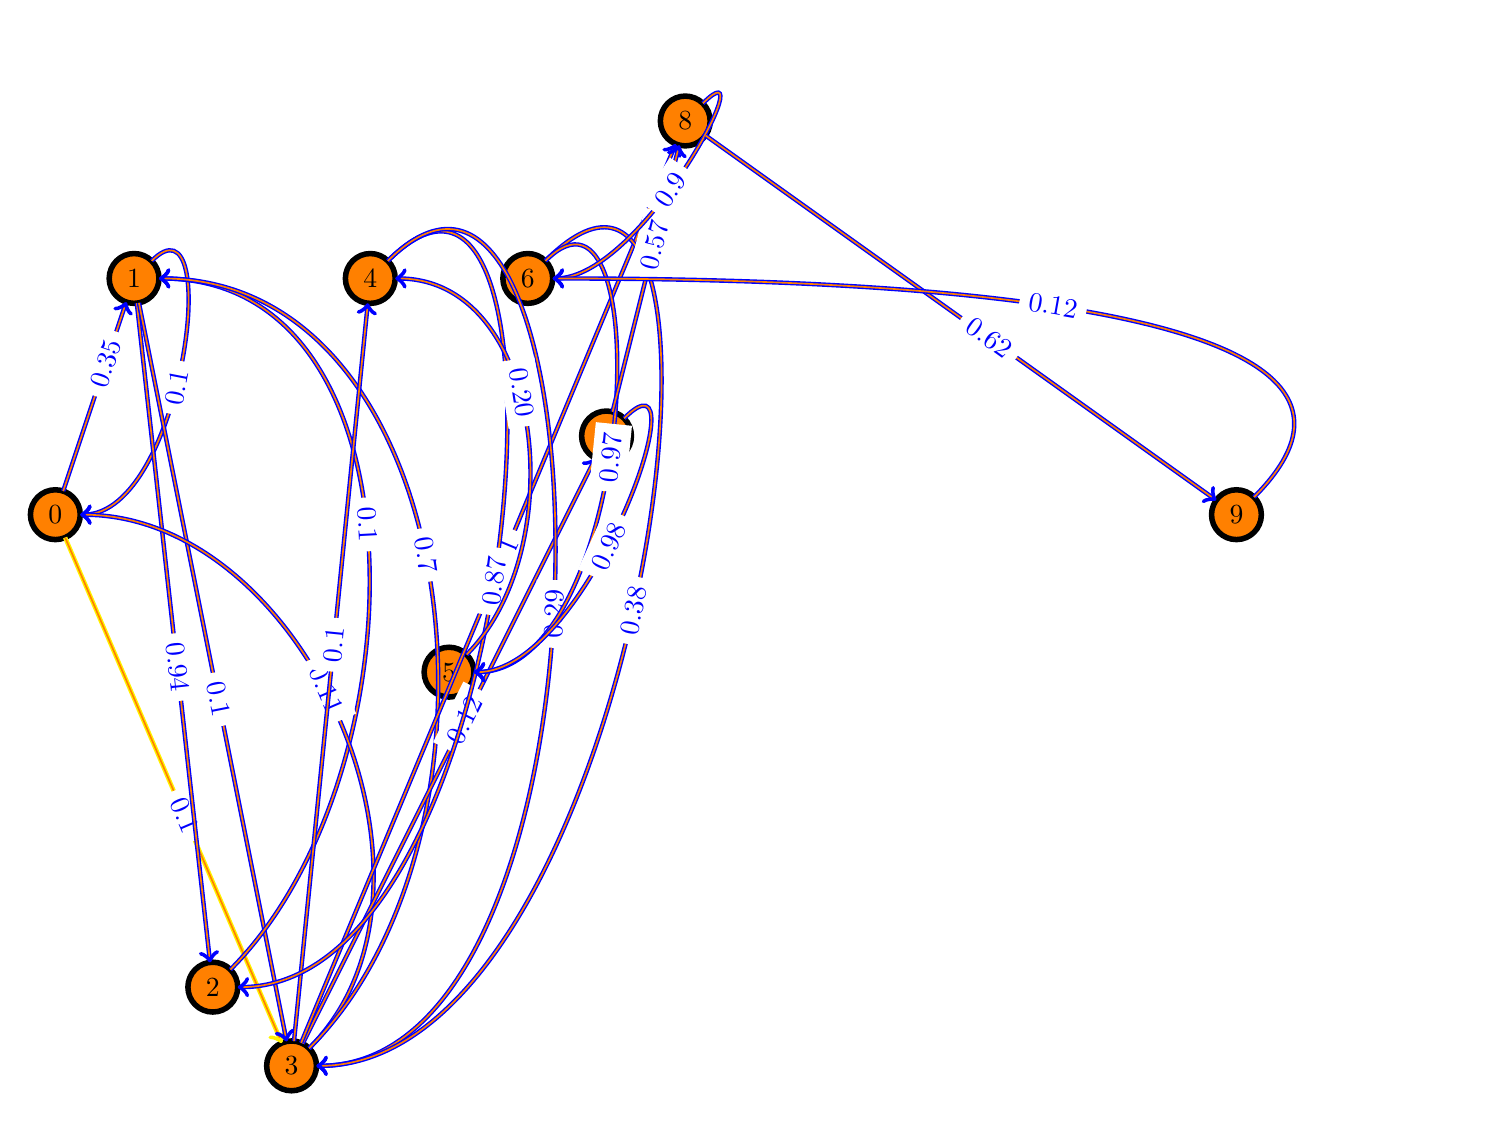
\begin{tikzpicture}
\SetVertexNormal[Shape      = circle,
FillColor  = orange,
LineWidth  = 2pt]
\SetUpEdge[lw         = 0.5pt,
color      = black,
labelcolor = white,
labeltext  = red,
labelstyle = {sloped,text=blue}]
\tikzstyle{TempStyle}=[double = orange]
\Vertex[x=-10, y=8]{0}
\Vertex[x=-9, y=11]{1}
\Vertex[x=-8, y=2]{2}
\Vertex[x=-7, y=1]{3}
\Vertex[x=-6, y=11]{4}
\Vertex[x=-5, y=6]{5}
\Vertex[x=-4, y=11]{6}
\Vertex[x=-3, y=9]{7}
\Vertex[x=-2, y=13]{8}
\Vertex[x=5, y=8]{9}
\tikzset{EdgeStyle/.style={->,TempStyle,relative=false,right=60,color=blue}}
\Edge[label=$0.35$](0)(1)
\tikzset{EdgeStyle/.style={->,TempStyle,relative=false,right=60,color=yellow}}
\Edge[label=$0.1$](0)(3)
\tikzset{EdgeStyle/.style={->,TempStyle,relative=false,left=60,color=blue,in=0,draw}}
\Edge[label=$0.1$](1)(0)
\tikzset{EdgeStyle/.style={->,TempStyle,relative=false,right=60,color=blue}}
\Edge[label=$0.94$](1)(2)
\tikzset{EdgeStyle/.style={->,TempStyle,relative=false,right=60,color=blue}}
\Edge[label=$0.1$](1)(3)
\tikzset{EdgeStyle/.style={->,TempStyle,relative=false,left=60,color=blue,in=0,draw}}
\Edge[label=$0.1$](2)(1)
\tikzset{EdgeStyle/.style={->,TempStyle,relative=false,left=60,color=blue,in=0,draw}}
\Edge[label=$0.11$](3)(0)
\tikzset{EdgeStyle/.style={->,TempStyle,relative=false,left=60,color=blue,in=0,draw}}
\Edge[label=$0.7$](3)(1)
\tikzset{EdgeStyle/.style={->,TempStyle,relative=false,right=60,color=blue}}
\Edge[label=$0.1$](3)(4)
\tikzset{EdgeStyle/.style={->,TempStyle,relative=false,right=60,color=blue}}
\Edge[label=$0.12$](3)(7)
\tikzset{EdgeStyle/.style={->,TempStyle,relative=false,right=60,color=blue}}
\Edge[label=$0.61$](3)(8)
\tikzset{EdgeStyle/.style={->,TempStyle,relative=false,left=60,color=blue,in=0,draw}}
\Edge[label=$0.87$](4)(2)
\tikzset{EdgeStyle/.style={->,TempStyle,relative=false,left=60,color=blue,in=0,draw}}
\Edge[label=$0.29$](4)(3)
\tikzset{EdgeStyle/.style={->,TempStyle,relative=false,left=60,color=blue,in=0,draw}}
\Edge[label=$0.20$](5)(4)
\tikzset{EdgeStyle/.style={->,TempStyle,relative=false,left=60,color=blue,in=0,draw}}
\Edge[label=$0.38$](6)(3)
\tikzset{EdgeStyle/.style={->,TempStyle,relative=false,left=60,color=blue,in=0,draw}}
\Edge[label=$0.97$](6)(5)
\tikzset{EdgeStyle/.style={->,TempStyle,relative=false,left=60,color=blue,in=0,draw}}
\Edge[label=$0.98$](7)(5)
\tikzset{EdgeStyle/.style={->,TempStyle,relative=false,right=60,color=blue}}
\Edge[label=$0.57$](7)(8)
\tikzset{EdgeStyle/.style={->,TempStyle,relative=false,left=60,color=blue,in=0,draw}}
\Edge[label=$0.9$](8)(6)
\tikzset{EdgeStyle/.style={->,TempStyle,relative=false,right=60,color=blue}}
\Edge[label=$0.62$](8)(9)
\tikzset{EdgeStyle/.style={->,TempStyle,relative=false,left=60,color=blue,in=0,draw}}
\Edge[label=$0.12$](9)(6)
\end{tikzpicture}\\
\begin{center}\begin{tabular}{l c}\\
\textcolor{orange}{\LARGE$\rightarrow$} & Chemin \\
 \textcolor{red}{\LARGE$\rightarrow$} & Créations arcs\\
 \textcolor{green}{\LARGE$\rightarrow$} & Modification flot\\
\end{tabular}
\end{center}
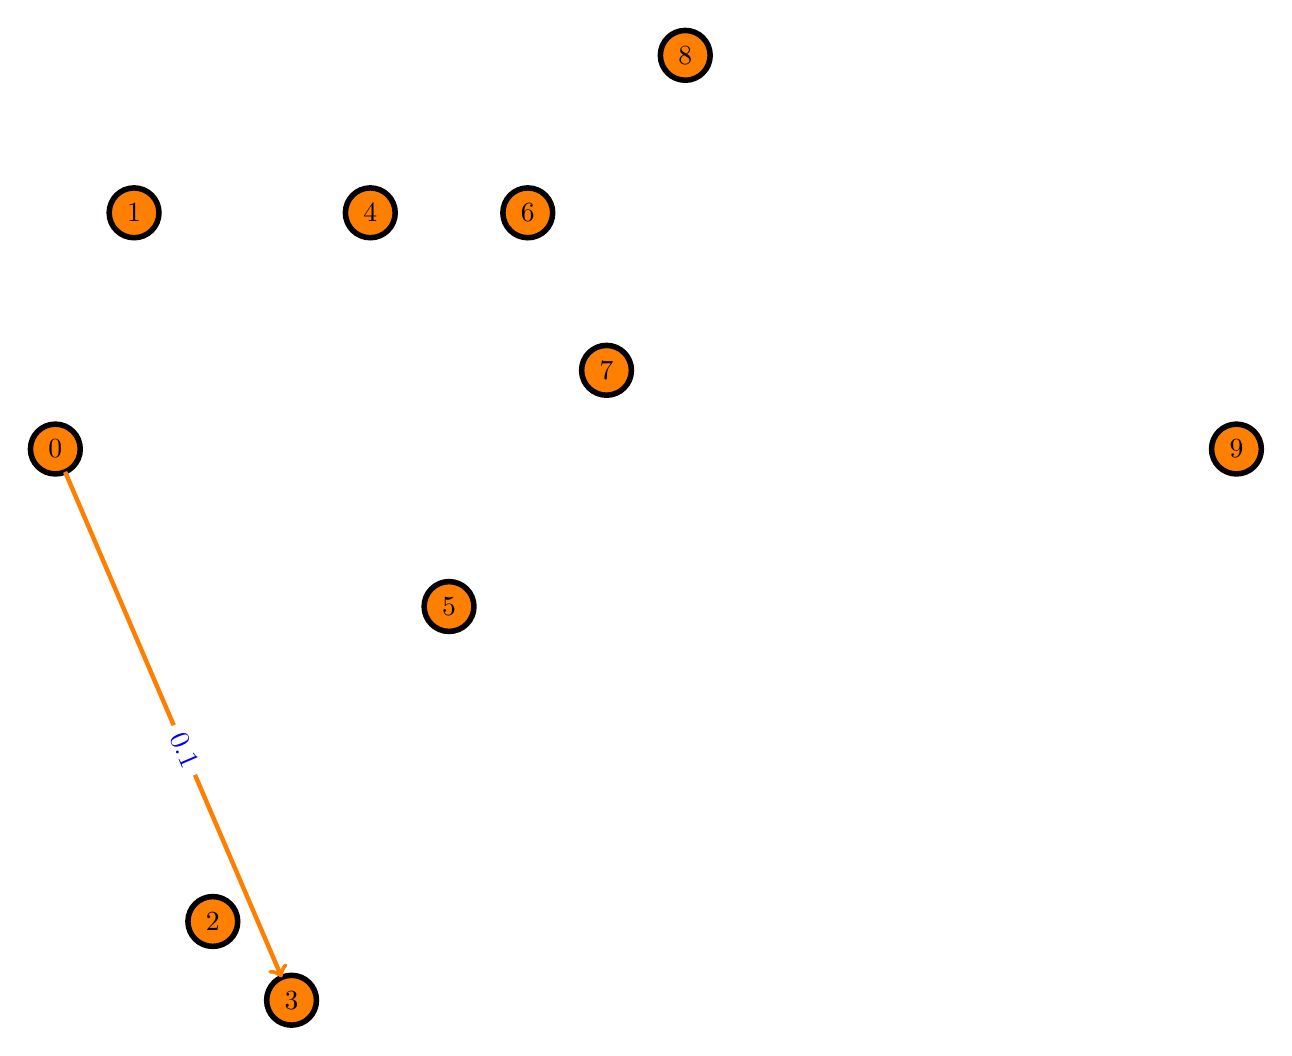
\begin{tikzpicture}
\SetVertexNormal[Shape      = circle,
FillColor  = orange,
LineWidth  = 2pt]
\SetUpEdge[lw         = 0.5pt,
color      = black,
labelcolor = white,
labeltext  = red,
labelstyle = {sloped,text=blue}]
\tikzstyle{TempStyle}=[double = orange]
\Vertex[x=-10, y=8]{0}
\Vertex[x=-9, y=11]{1}
\Vertex[x=-8, y=2]{2}
\Vertex[x=-7, y=1]{3}
\Vertex[x=-6, y=11]{4}
\Vertex[x=-5, y=6]{5}
\Vertex[x=-4, y=11]{6}
\Vertex[x=-3, y=9]{7}
\Vertex[x=-2, y=13]{8}
\Vertex[x=5, y=8]{9}
\tikzset{EdgeStyle/.style={->,TempStyle,relative=false,right=60,color=orange}}
\Edge[label=$0.1$](0)(3)
\end{tikzpicture}\\
\begin{center}\begin{tabular}{l c}\\
\textcolor{orange}{\LARGE$\rightarrow$} & Chemin \\
 \textcolor{red}{\LARGE$\rightarrow$} & Créations arcs\\
 \textcolor{green}{\LARGE$\rightarrow$} & Modification flot\\
\end{tabular}
\end{center}
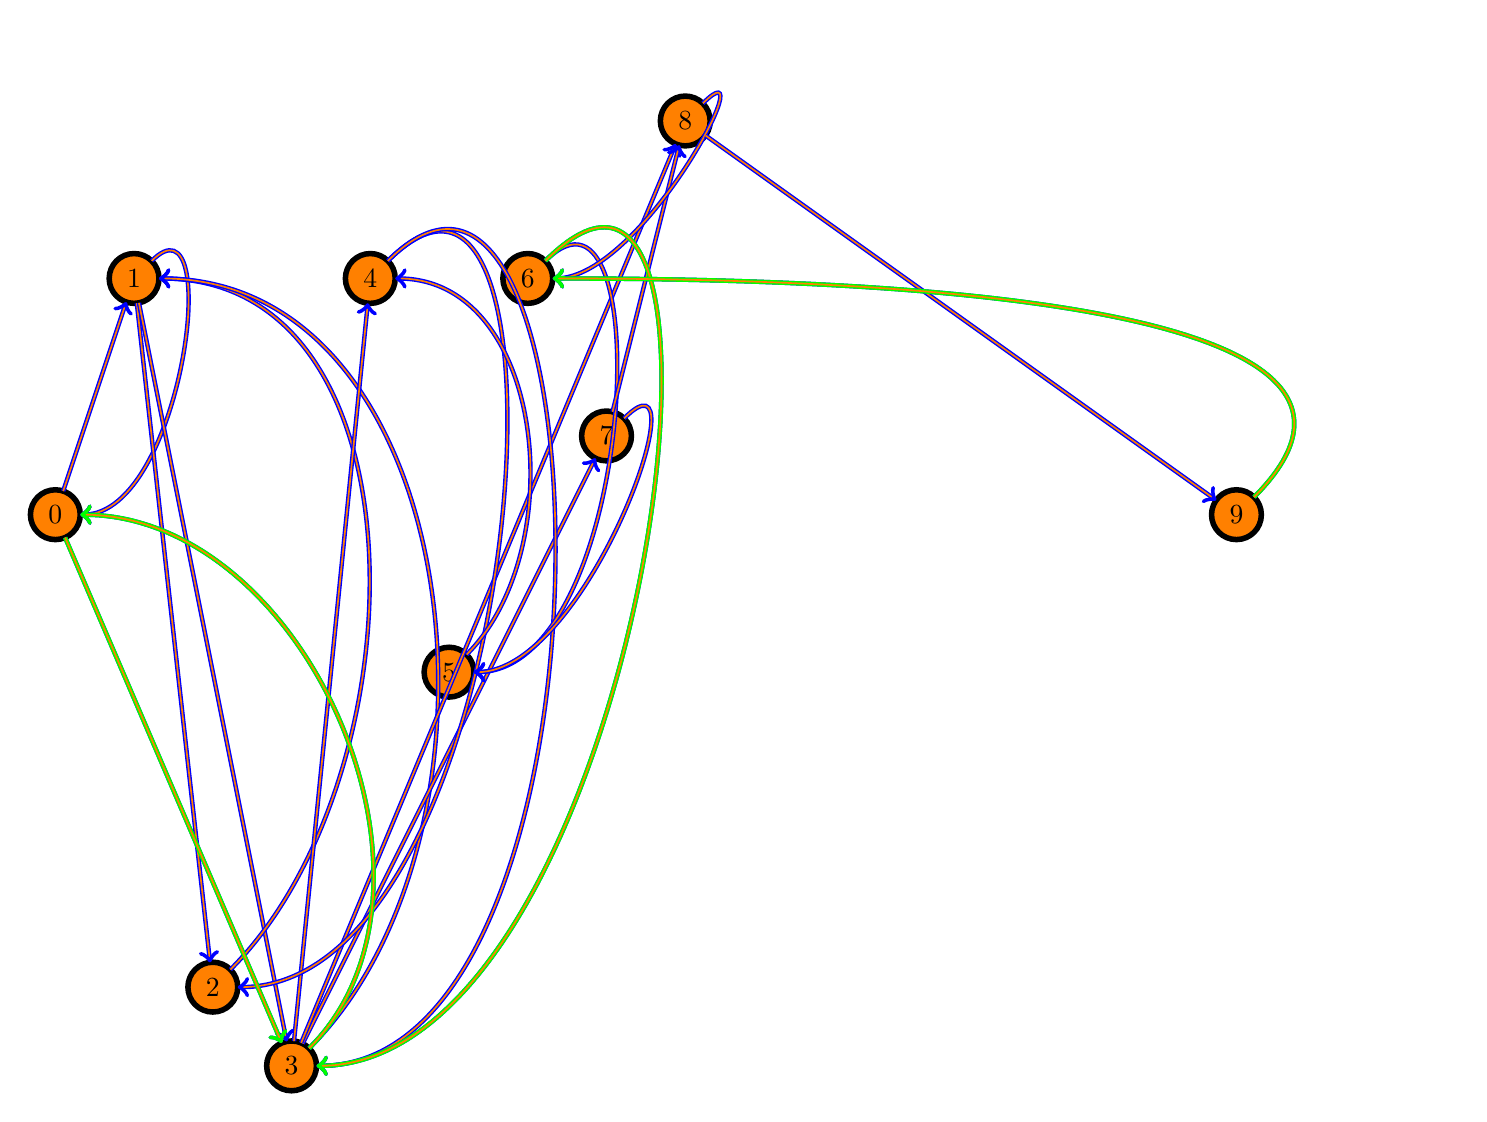
\begin{tikzpicture}
\SetVertexNormal[Shape      = circle,
FillColor  = orange,
LineWidth  = 2pt]
\SetUpEdge[lw         = 0.5pt,
color      = black,
labelcolor = white,
labeltext  = red,
labelstyle = {sloped,text=blue}]
\tikzstyle{TempStyle}=[double = orange]
\Vertex[x=-10, y=8]{0}
\Vertex[x=-9, y=11]{1}
\Vertex[x=-8, y=2]{2}
\Vertex[x=-7, y=1]{3}
\Vertex[x=-6, y=11]{4}
\Vertex[x=-5, y=6]{5}
\Vertex[x=-4, y=11]{6}
\Vertex[x=-3, y=9]{7}
\Vertex[x=-2, y=13]{8}
\Vertex[x=5, y=8]{9}
\tikzset{EdgeStyle/.style={->,TempStyle,relative=false,right=60,color=blue}}
\Edge(0)(1)
\tikzset{EdgeStyle/.style={->,TempStyle,relative=false,right=60,color=blue}}
\Edge(0)(3)
\tikzset{EdgeStyle/.style={->,TempStyle,relative=false,left=60,color=blue,in=0,draw}}
\Edge(1)(0)
\tikzset{EdgeStyle/.style={->,TempStyle,relative=false,right=60,color=blue}}
\Edge(1)(2)
\tikzset{EdgeStyle/.style={->,TempStyle,relative=false,right=60,color=blue}}
\Edge(1)(3)
\tikzset{EdgeStyle/.style={->,TempStyle,relative=false,left=60,color=blue,in=0,draw}}
\Edge(2)(1)
\tikzset{EdgeStyle/.style={->,TempStyle,relative=false,left=60,color=blue,in=0,draw}}
\Edge(3)(0)
\tikzset{EdgeStyle/.style={->,TempStyle,relative=false,left=60,color=blue,in=0,draw}}
\Edge(3)(1)
\tikzset{EdgeStyle/.style={->,TempStyle,relative=false,right=60,color=blue}}
\Edge(3)(4)
\tikzset{EdgeStyle/.style={->,TempStyle,relative=false,right=60,color=blue}}
\Edge(3)(7)
\tikzset{EdgeStyle/.style={->,TempStyle,relative=false,right=60,color=blue}}
\Edge(3)(8)
\tikzset{EdgeStyle/.style={->,TempStyle,relative=false,left=60,color=blue,in=0,draw}}
\Edge(4)(2)
\tikzset{EdgeStyle/.style={->,TempStyle,relative=false,left=60,color=blue,in=0,draw}}
\Edge(4)(3)
\tikzset{EdgeStyle/.style={->,TempStyle,relative=false,left=60,color=blue,in=0,draw}}
\Edge(5)(4)
\tikzset{EdgeStyle/.style={->,TempStyle,relative=false,left=60,color=blue,in=0,draw}}
\Edge(6)(3)
\tikzset{EdgeStyle/.style={->,TempStyle,relative=false,left=60,color=blue,in=0,draw}}
\Edge(6)(5)
\tikzset{EdgeStyle/.style={->,TempStyle,relative=false,left=60,color=blue,in=0,draw}}
\Edge(7)(5)
\tikzset{EdgeStyle/.style={->,TempStyle,relative=false,right=60,color=blue}}
\Edge(7)(8)
\tikzset{EdgeStyle/.style={->,TempStyle,relative=false,left=60,color=blue,in=0,draw}}
\Edge(8)(6)
\tikzset{EdgeStyle/.style={->,TempStyle,relative=false,right=60,color=blue}}
\Edge(8)(9)
\tikzset{EdgeStyle/.style={->,TempStyle,relative=false,left=60,color=blue,in=0,draw}}
\Edge(9)(6)
\tikzset{EdgeStyle/.style={->,TempStyle,relative=false,right=60,color=green}}
\Edge(0)(3)
\tikzset{EdgeStyle/.style={->,TempStyle,relative=false,right=60,in=0,color=green}}
\Edge(3)(0)
\tikzset{EdgeStyle/.style={->,TempStyle,relative=false,right=60,in=0,color=green}}
\Edge(6)(3)
\tikzset{EdgeStyle/.style={->,TempStyle,relative=false,right=60,in=0,color=green}}
\Edge(9)(6)
\end{tikzpicture}\\
\begin{center}\begin{tabular}{l c}\\
\textcolor{orange}{\LARGE$\rightarrow$} & Chemin \\
 \textcolor{red}{\LARGE$\rightarrow$} & Créations arcs\\
 \textcolor{green}{\LARGE$\rightarrow$} & Modification flot\\
\end{tabular}
\end{center}
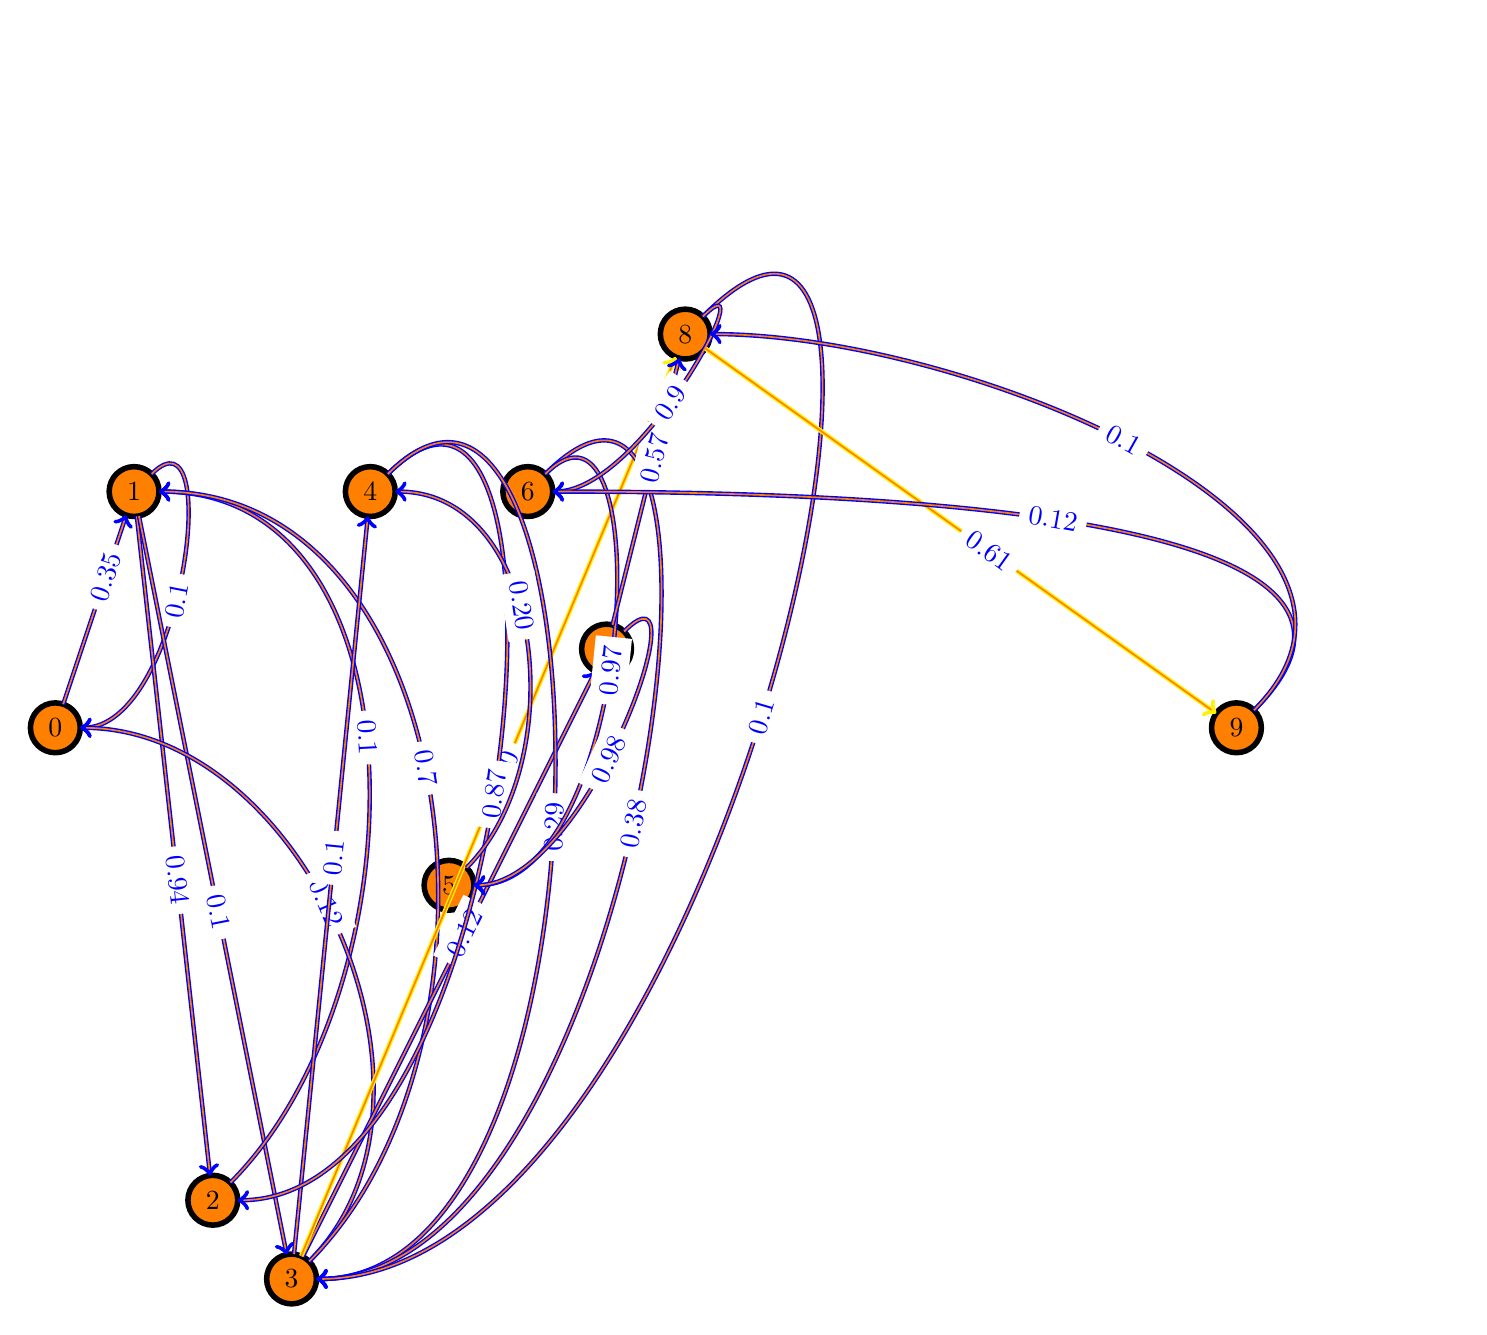
\begin{tikzpicture}
\SetVertexNormal[Shape      = circle,
FillColor  = orange,
LineWidth  = 2pt]
\SetUpEdge[lw         = 0.5pt,
color      = black,
labelcolor = white,
labeltext  = red,
labelstyle = {sloped,text=blue}]
\tikzstyle{TempStyle}=[double = orange]
\Vertex[x=-10, y=8]{0}
\Vertex[x=-9, y=11]{1}
\Vertex[x=-8, y=2]{2}
\Vertex[x=-7, y=1]{3}
\Vertex[x=-6, y=11]{4}
\Vertex[x=-5, y=6]{5}
\Vertex[x=-4, y=11]{6}
\Vertex[x=-3, y=9]{7}
\Vertex[x=-2, y=13]{8}
\Vertex[x=5, y=8]{9}
\tikzset{EdgeStyle/.style={->,TempStyle,relative=false,right=60,color=blue}}
\Edge[label=$0.35$](0)(1)
\tikzset{EdgeStyle/.style={->,TempStyle,relative=false,left=60,color=blue,in=0,draw}}
\Edge[label=$0.1$](1)(0)
\tikzset{EdgeStyle/.style={->,TempStyle,relative=false,right=60,color=blue}}
\Edge[label=$0.94$](1)(2)
\tikzset{EdgeStyle/.style={->,TempStyle,relative=false,right=60,color=blue}}
\Edge[label=$0.1$](1)(3)
\tikzset{EdgeStyle/.style={->,TempStyle,relative=false,left=60,color=blue,in=0,draw}}
\Edge[label=$0.1$](2)(1)
\tikzset{EdgeStyle/.style={->,TempStyle,relative=false,left=60,color=blue,in=0,draw}}
\Edge[label=$0.12$](3)(0)
\tikzset{EdgeStyle/.style={->,TempStyle,relative=false,left=60,color=blue,in=0,draw}}
\Edge[label=$0.7$](3)(1)
\tikzset{EdgeStyle/.style={->,TempStyle,relative=false,right=60,color=blue}}
\Edge[label=$0.1$](3)(4)
\tikzset{EdgeStyle/.style={->,TempStyle,relative=false,right=60,color=blue}}
\Edge[label=$0.12$](3)(7)
\tikzset{EdgeStyle/.style={->,TempStyle,relative=false,right=60,color=yellow}}
\Edge[label=$0.60$](3)(8)
\tikzset{EdgeStyle/.style={->,TempStyle,relative=false,left=60,color=blue,in=0,draw}}
\Edge[label=$0.87$](4)(2)
\tikzset{EdgeStyle/.style={->,TempStyle,relative=false,left=60,color=blue,in=0,draw}}
\Edge[label=$0.29$](4)(3)
\tikzset{EdgeStyle/.style={->,TempStyle,relative=false,left=60,color=blue,in=0,draw}}
\Edge[label=$0.20$](5)(4)
\tikzset{EdgeStyle/.style={->,TempStyle,relative=false,left=60,color=blue,in=0,draw}}
\Edge[label=$0.38$](6)(3)
\tikzset{EdgeStyle/.style={->,TempStyle,relative=false,left=60,color=blue,in=0,draw}}
\Edge[label=$0.97$](6)(5)
\tikzset{EdgeStyle/.style={->,TempStyle,relative=false,left=60,color=blue,in=0,draw}}
\Edge[label=$0.98$](7)(5)
\tikzset{EdgeStyle/.style={->,TempStyle,relative=false,right=60,color=blue}}
\Edge[label=$0.57$](7)(8)
\tikzset{EdgeStyle/.style={->,TempStyle,relative=false,left=60,color=blue,in=0,draw}}
\Edge[label=$0.1$](8)(3)
\tikzset{EdgeStyle/.style={->,TempStyle,relative=false,left=60,color=blue,in=0,draw}}
\Edge[label=$0.9$](8)(6)
\tikzset{EdgeStyle/.style={->,TempStyle,relative=false,right=60,color=yellow}}
\Edge[label=$0.61$](8)(9)
\tikzset{EdgeStyle/.style={->,TempStyle,relative=false,left=60,color=blue,in=0,draw}}
\Edge[label=$0.12$](9)(6)
\tikzset{EdgeStyle/.style={->,TempStyle,relative=false,left=60,color=blue,in=0,draw}}
\Edge[label=$0.1$](9)(8)
\end{tikzpicture}\\
\begin{center}\begin{tabular}{l c}\\
\textcolor{orange}{\LARGE$\rightarrow$} & Chemin \\
 \textcolor{red}{\LARGE$\rightarrow$} & Créations arcs\\
 \textcolor{green}{\LARGE$\rightarrow$} & Modification flot\\
\end{tabular}
\end{center}
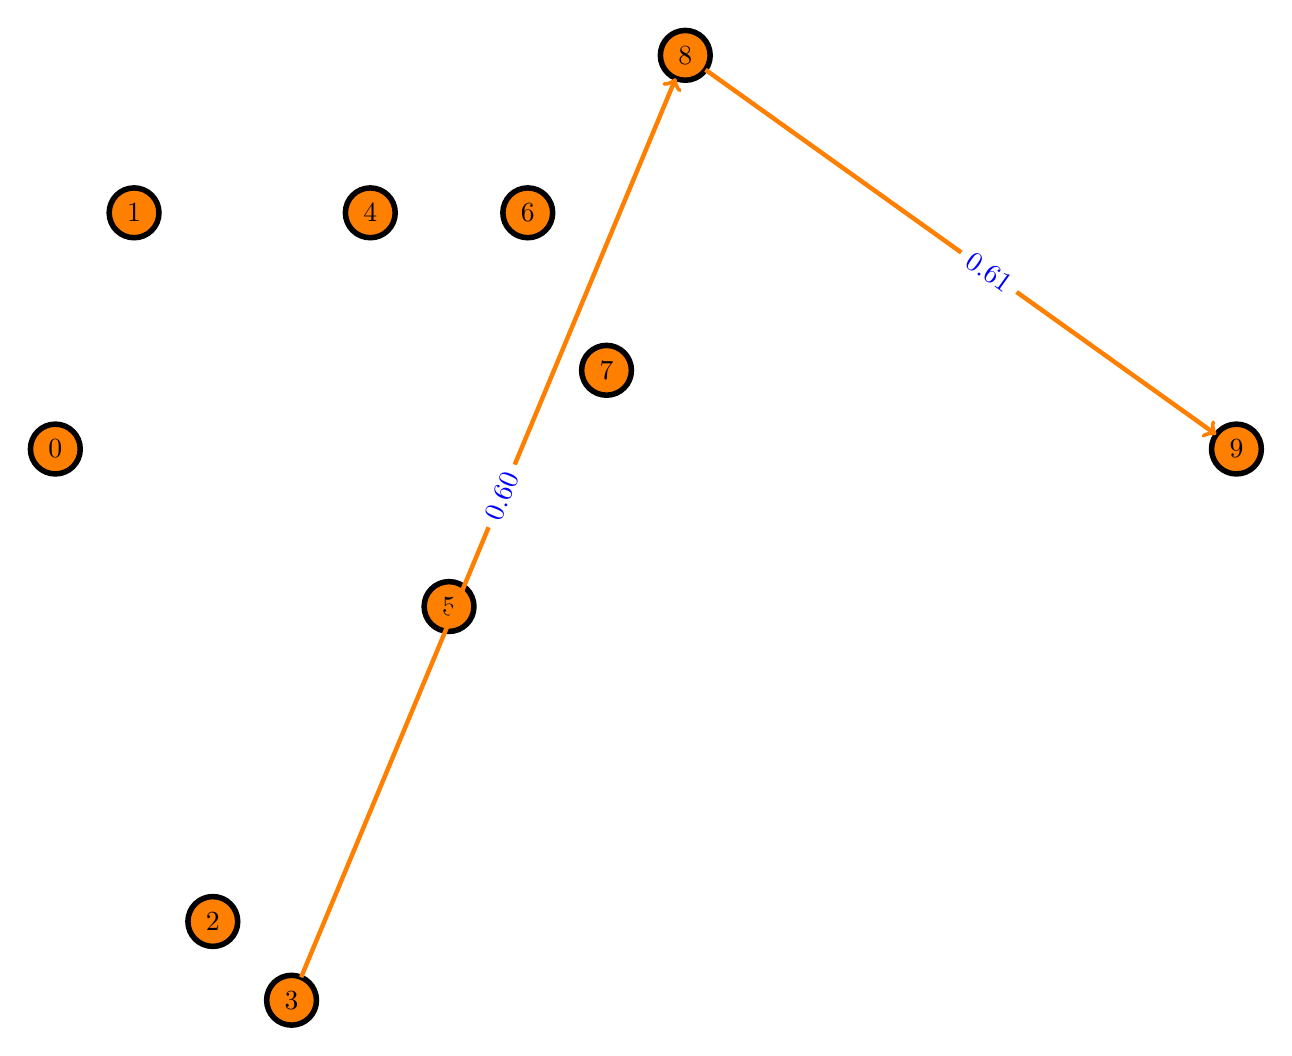
\begin{tikzpicture}
\SetVertexNormal[Shape      = circle,
FillColor  = orange,
LineWidth  = 2pt]
\SetUpEdge[lw         = 0.5pt,
color      = black,
labelcolor = white,
labeltext  = red,
labelstyle = {sloped,text=blue}]
\tikzstyle{TempStyle}=[double = orange]
\Vertex[x=-10, y=8]{0}
\Vertex[x=-9, y=11]{1}
\Vertex[x=-8, y=2]{2}
\Vertex[x=-7, y=1]{3}
\Vertex[x=-6, y=11]{4}
\Vertex[x=-5, y=6]{5}
\Vertex[x=-4, y=11]{6}
\Vertex[x=-3, y=9]{7}
\Vertex[x=-2, y=13]{8}
\Vertex[x=5, y=8]{9}
\tikzset{EdgeStyle/.style={->,TempStyle,relative=false,right=60,color=orange}}
\Edge[label=$0.60$](3)(8)
\tikzset{EdgeStyle/.style={->,TempStyle,relative=false,right=60,color=orange}}
\Edge[label=$0.61$](8)(9)
\end{tikzpicture}\\
\begin{center}\begin{tabular}{l c}\\
\textcolor{orange}{\LARGE$\rightarrow$} & Chemin \\
 \textcolor{red}{\LARGE$\rightarrow$} & Créations arcs\\
 \textcolor{green}{\LARGE$\rightarrow$} & Modification flot\\
\end{tabular}
\end{center}
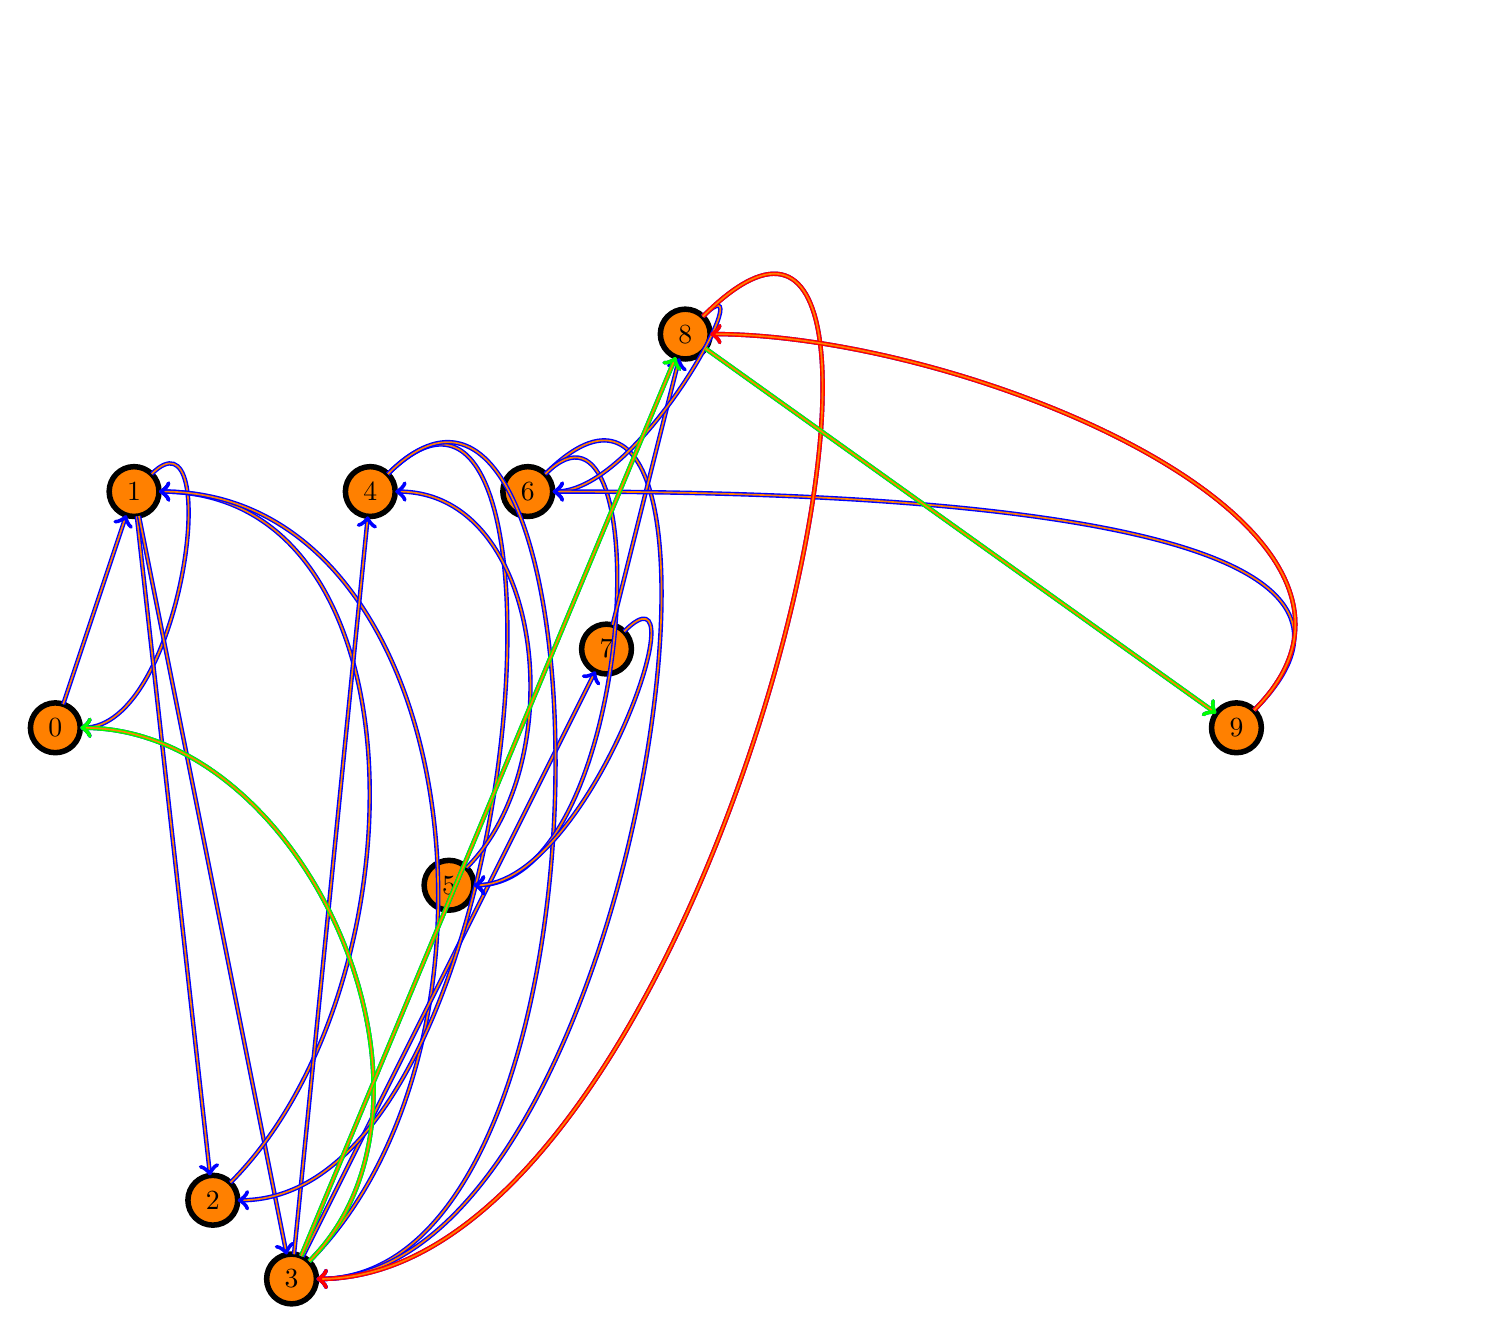
\begin{tikzpicture}
\SetVertexNormal[Shape      = circle,
FillColor  = orange,
LineWidth  = 2pt]
\SetUpEdge[lw         = 0.5pt,
color      = black,
labelcolor = white,
labeltext  = red,
labelstyle = {sloped,text=blue}]
\tikzstyle{TempStyle}=[double = orange]
\Vertex[x=-10, y=8]{0}
\Vertex[x=-9, y=11]{1}
\Vertex[x=-8, y=2]{2}
\Vertex[x=-7, y=1]{3}
\Vertex[x=-6, y=11]{4}
\Vertex[x=-5, y=6]{5}
\Vertex[x=-4, y=11]{6}
\Vertex[x=-3, y=9]{7}
\Vertex[x=-2, y=13]{8}
\Vertex[x=5, y=8]{9}
\tikzset{EdgeStyle/.style={->,TempStyle,relative=false,right=60,color=blue}}
\Edge(0)(1)
\tikzset{EdgeStyle/.style={->,TempStyle,relative=false,left=60,color=blue,in=0,draw}}
\Edge(1)(0)
\tikzset{EdgeStyle/.style={->,TempStyle,relative=false,right=60,color=blue}}
\Edge(1)(2)
\tikzset{EdgeStyle/.style={->,TempStyle,relative=false,right=60,color=blue}}
\Edge(1)(3)
\tikzset{EdgeStyle/.style={->,TempStyle,relative=false,left=60,color=blue,in=0,draw}}
\Edge(2)(1)
\tikzset{EdgeStyle/.style={->,TempStyle,relative=false,left=60,color=blue,in=0,draw}}
\Edge(3)(0)
\tikzset{EdgeStyle/.style={->,TempStyle,relative=false,left=60,color=blue,in=0,draw}}
\Edge(3)(1)
\tikzset{EdgeStyle/.style={->,TempStyle,relative=false,right=60,color=blue}}
\Edge(3)(4)
\tikzset{EdgeStyle/.style={->,TempStyle,relative=false,right=60,color=blue}}
\Edge(3)(7)
\tikzset{EdgeStyle/.style={->,TempStyle,relative=false,right=60,color=blue}}
\Edge(3)(8)
\tikzset{EdgeStyle/.style={->,TempStyle,relative=false,left=60,color=blue,in=0,draw}}
\Edge(4)(2)
\tikzset{EdgeStyle/.style={->,TempStyle,relative=false,left=60,color=blue,in=0,draw}}
\Edge(4)(3)
\tikzset{EdgeStyle/.style={->,TempStyle,relative=false,left=60,color=blue,in=0,draw}}
\Edge(5)(4)
\tikzset{EdgeStyle/.style={->,TempStyle,relative=false,left=60,color=blue,in=0,draw}}
\Edge(6)(3)
\tikzset{EdgeStyle/.style={->,TempStyle,relative=false,left=60,color=blue,in=0,draw}}
\Edge(6)(5)
\tikzset{EdgeStyle/.style={->,TempStyle,relative=false,left=60,color=blue,in=0,draw}}
\Edge(7)(5)
\tikzset{EdgeStyle/.style={->,TempStyle,relative=false,right=60,color=blue}}
\Edge(7)(8)
\tikzset{EdgeStyle/.style={->,TempStyle,relative=false,left=60,color=blue,in=0,draw}}
\Edge(8)(3)
\tikzset{EdgeStyle/.style={->,TempStyle,relative=false,left=60,color=blue,in=0,draw}}
\Edge(8)(6)
\tikzset{EdgeStyle/.style={->,TempStyle,relative=false,right=60,color=blue}}
\Edge(8)(9)
\tikzset{EdgeStyle/.style={->,TempStyle,relative=false,left=60,color=blue,in=0,draw}}
\Edge(9)(6)
\tikzset{EdgeStyle/.style={->,TempStyle,relative=false,left=60,color=blue,in=0,draw}}
\Edge(9)(8)
\tikzset{EdgeStyle/.style={->,TempStyle,relative=false,right=60,in=0,color=green}}
\Edge(3)(0)
\tikzset{EdgeStyle/.style={->,TempStyle,relative=false,right=60,color=green}}
\Edge(3)(8)
\tikzset{EdgeStyle/.style={->,TempStyle,relative=false,right=60,in=0,color=red}}
\Edge(8)(3)
\tikzset{EdgeStyle/.style={->,TempStyle,relative=false,right=60,color=green}}
\Edge(8)(9)
\tikzset{EdgeStyle/.style={->,TempStyle,relative=false,right=60,in=0,color=red}}
\Edge(9)(8)
\end{tikzpicture}\\
\begin{center}\begin{tabular}{l c}\\
\textcolor{orange}{\LARGE$\rightarrow$} & Chemin \\
 \textcolor{red}{\LARGE$\rightarrow$} & Créations arcs\\
 \textcolor{green}{\LARGE$\rightarrow$} & Modification flot\\
\end{tabular}
\end{center}
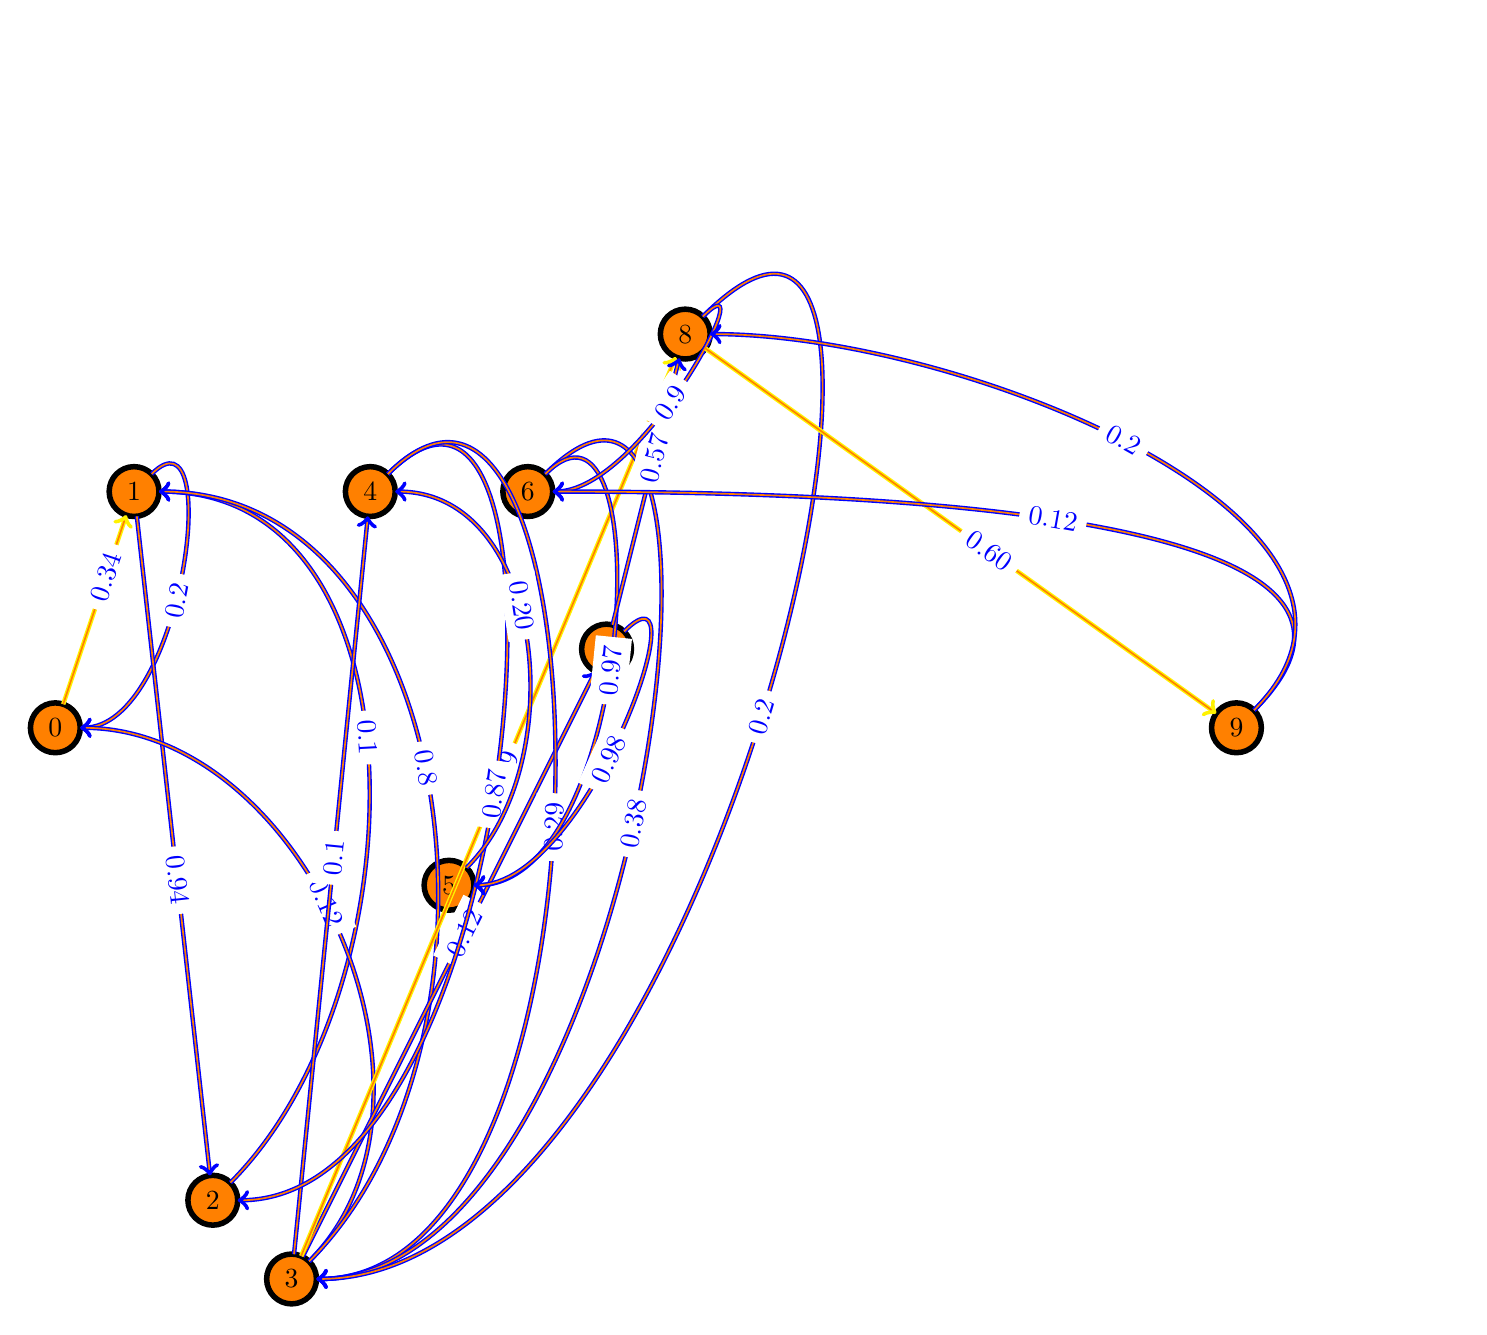
\begin{tikzpicture}
\SetVertexNormal[Shape      = circle,
FillColor  = orange,
LineWidth  = 2pt]
\SetUpEdge[lw         = 0.5pt,
color      = black,
labelcolor = white,
labeltext  = red,
labelstyle = {sloped,text=blue}]
\tikzstyle{TempStyle}=[double = orange]
\Vertex[x=-10, y=8]{0}
\Vertex[x=-9, y=11]{1}
\Vertex[x=-8, y=2]{2}
\Vertex[x=-7, y=1]{3}
\Vertex[x=-6, y=11]{4}
\Vertex[x=-5, y=6]{5}
\Vertex[x=-4, y=11]{6}
\Vertex[x=-3, y=9]{7}
\Vertex[x=-2, y=13]{8}
\Vertex[x=5, y=8]{9}
\tikzset{EdgeStyle/.style={->,TempStyle,relative=false,right=60,color=yellow}}
\Edge[label=$0.34$](0)(1)
\tikzset{EdgeStyle/.style={->,TempStyle,relative=false,left=60,color=blue,in=0,draw}}
\Edge[label=$0.2$](1)(0)
\tikzset{EdgeStyle/.style={->,TempStyle,relative=false,right=60,color=blue}}
\Edge[label=$0.94$](1)(2)
\tikzset{EdgeStyle/.style={->,TempStyle,relative=false,left=60,color=blue,in=0,draw}}
\Edge[label=$0.1$](2)(1)
\tikzset{EdgeStyle/.style={->,TempStyle,relative=false,left=60,color=blue,in=0,draw}}
\Edge[label=$0.12$](3)(0)
\tikzset{EdgeStyle/.style={->,TempStyle,relative=false,left=60,color=blue,in=0,draw}}
\Edge[label=$0.8$](3)(1)
\tikzset{EdgeStyle/.style={->,TempStyle,relative=false,right=60,color=blue}}
\Edge[label=$0.1$](3)(4)
\tikzset{EdgeStyle/.style={->,TempStyle,relative=false,right=60,color=blue}}
\Edge[label=$0.12$](3)(7)
\tikzset{EdgeStyle/.style={->,TempStyle,relative=false,right=60,color=yellow}}
\Edge[label=$0.59$](3)(8)
\tikzset{EdgeStyle/.style={->,TempStyle,relative=false,left=60,color=blue,in=0,draw}}
\Edge[label=$0.87$](4)(2)
\tikzset{EdgeStyle/.style={->,TempStyle,relative=false,left=60,color=blue,in=0,draw}}
\Edge[label=$0.29$](4)(3)
\tikzset{EdgeStyle/.style={->,TempStyle,relative=false,left=60,color=blue,in=0,draw}}
\Edge[label=$0.20$](5)(4)
\tikzset{EdgeStyle/.style={->,TempStyle,relative=false,left=60,color=blue,in=0,draw}}
\Edge[label=$0.38$](6)(3)
\tikzset{EdgeStyle/.style={->,TempStyle,relative=false,left=60,color=blue,in=0,draw}}
\Edge[label=$0.97$](6)(5)
\tikzset{EdgeStyle/.style={->,TempStyle,relative=false,left=60,color=blue,in=0,draw}}
\Edge[label=$0.98$](7)(5)
\tikzset{EdgeStyle/.style={->,TempStyle,relative=false,right=60,color=blue}}
\Edge[label=$0.57$](7)(8)
\tikzset{EdgeStyle/.style={->,TempStyle,relative=false,left=60,color=blue,in=0,draw}}
\Edge[label=$0.2$](8)(3)
\tikzset{EdgeStyle/.style={->,TempStyle,relative=false,left=60,color=blue,in=0,draw}}
\Edge[label=$0.9$](8)(6)
\tikzset{EdgeStyle/.style={->,TempStyle,relative=false,right=60,color=yellow}}
\Edge[label=$0.60$](8)(9)
\tikzset{EdgeStyle/.style={->,TempStyle,relative=false,left=60,color=blue,in=0,draw}}
\Edge[label=$0.12$](9)(6)
\tikzset{EdgeStyle/.style={->,TempStyle,relative=false,left=60,color=blue,in=0,draw}}
\Edge[label=$0.2$](9)(8)
\end{tikzpicture}\\
\begin{center}\begin{tabular}{l c}\\
\textcolor{orange}{\LARGE$\rightarrow$} & Chemin \\
 \textcolor{red}{\LARGE$\rightarrow$} & Créations arcs\\
 \textcolor{green}{\LARGE$\rightarrow$} & Modification flot\\
\end{tabular}
\end{center}
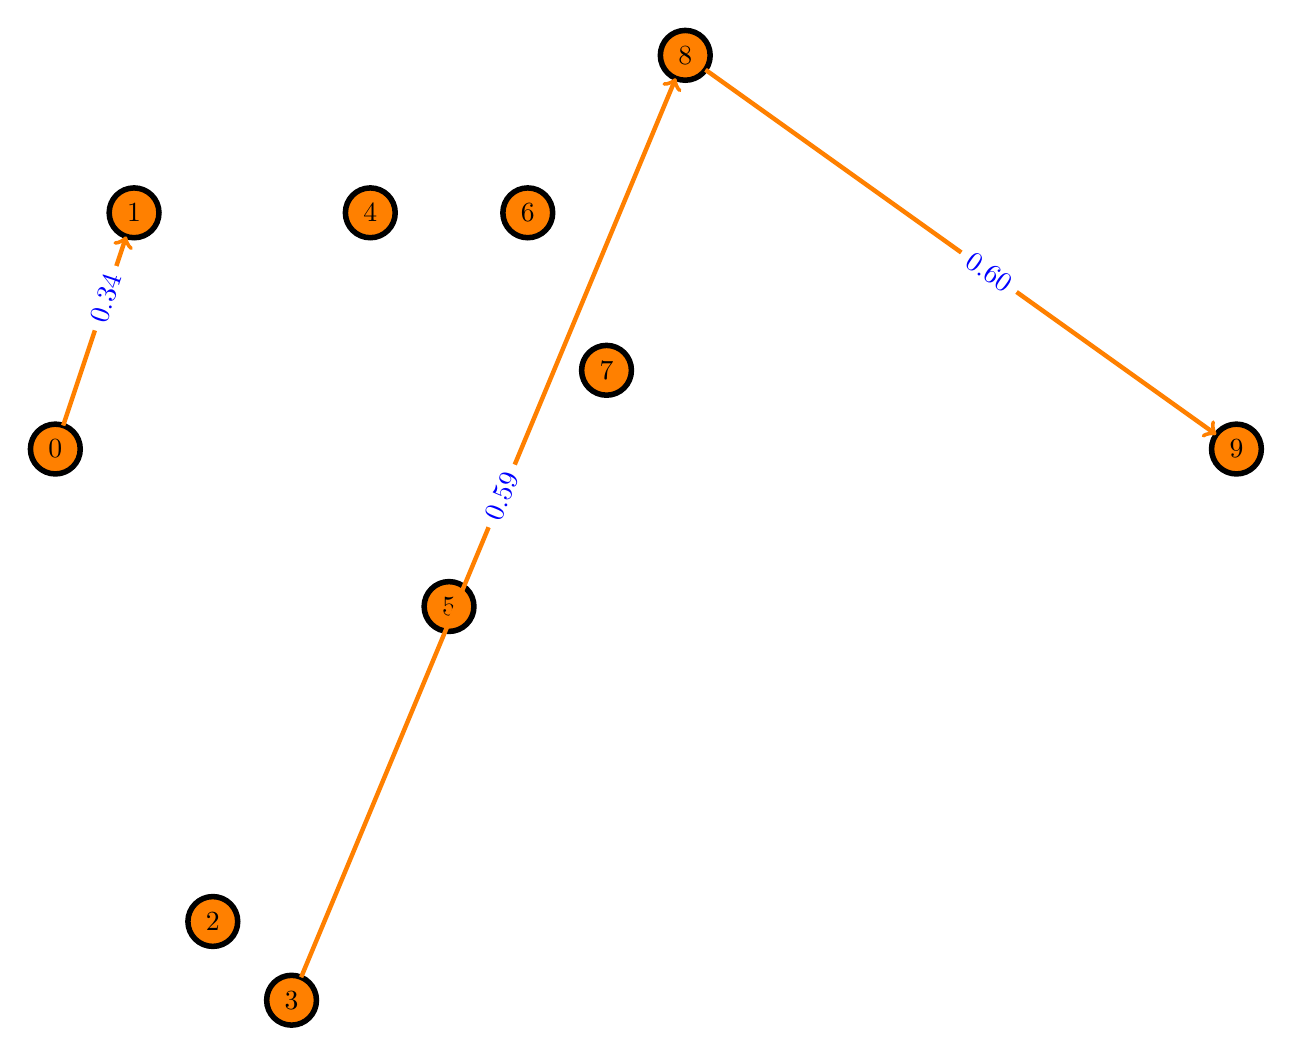
\begin{tikzpicture}
\SetVertexNormal[Shape      = circle,
FillColor  = orange,
LineWidth  = 2pt]
\SetUpEdge[lw         = 0.5pt,
color      = black,
labelcolor = white,
labeltext  = red,
labelstyle = {sloped,text=blue}]
\tikzstyle{TempStyle}=[double = orange]
\Vertex[x=-10, y=8]{0}
\Vertex[x=-9, y=11]{1}
\Vertex[x=-8, y=2]{2}
\Vertex[x=-7, y=1]{3}
\Vertex[x=-6, y=11]{4}
\Vertex[x=-5, y=6]{5}
\Vertex[x=-4, y=11]{6}
\Vertex[x=-3, y=9]{7}
\Vertex[x=-2, y=13]{8}
\Vertex[x=5, y=8]{9}
\tikzset{EdgeStyle/.style={->,TempStyle,relative=false,right=60,color=orange}}
\Edge[label=$0.34$](0)(1)
\tikzset{EdgeStyle/.style={->,TempStyle,relative=false,right=60,color=orange}}
\Edge[label=$0.59$](3)(8)
\tikzset{EdgeStyle/.style={->,TempStyle,relative=false,right=60,color=orange}}
\Edge[label=$0.60$](8)(9)
\end{tikzpicture}\\
\begin{center}\begin{tabular}{l c}\\
\textcolor{orange}{\LARGE$\rightarrow$} & Chemin \\
 \textcolor{red}{\LARGE$\rightarrow$} & Créations arcs\\
 \textcolor{green}{\LARGE$\rightarrow$} & Modification flot\\
\end{tabular}
\end{center}
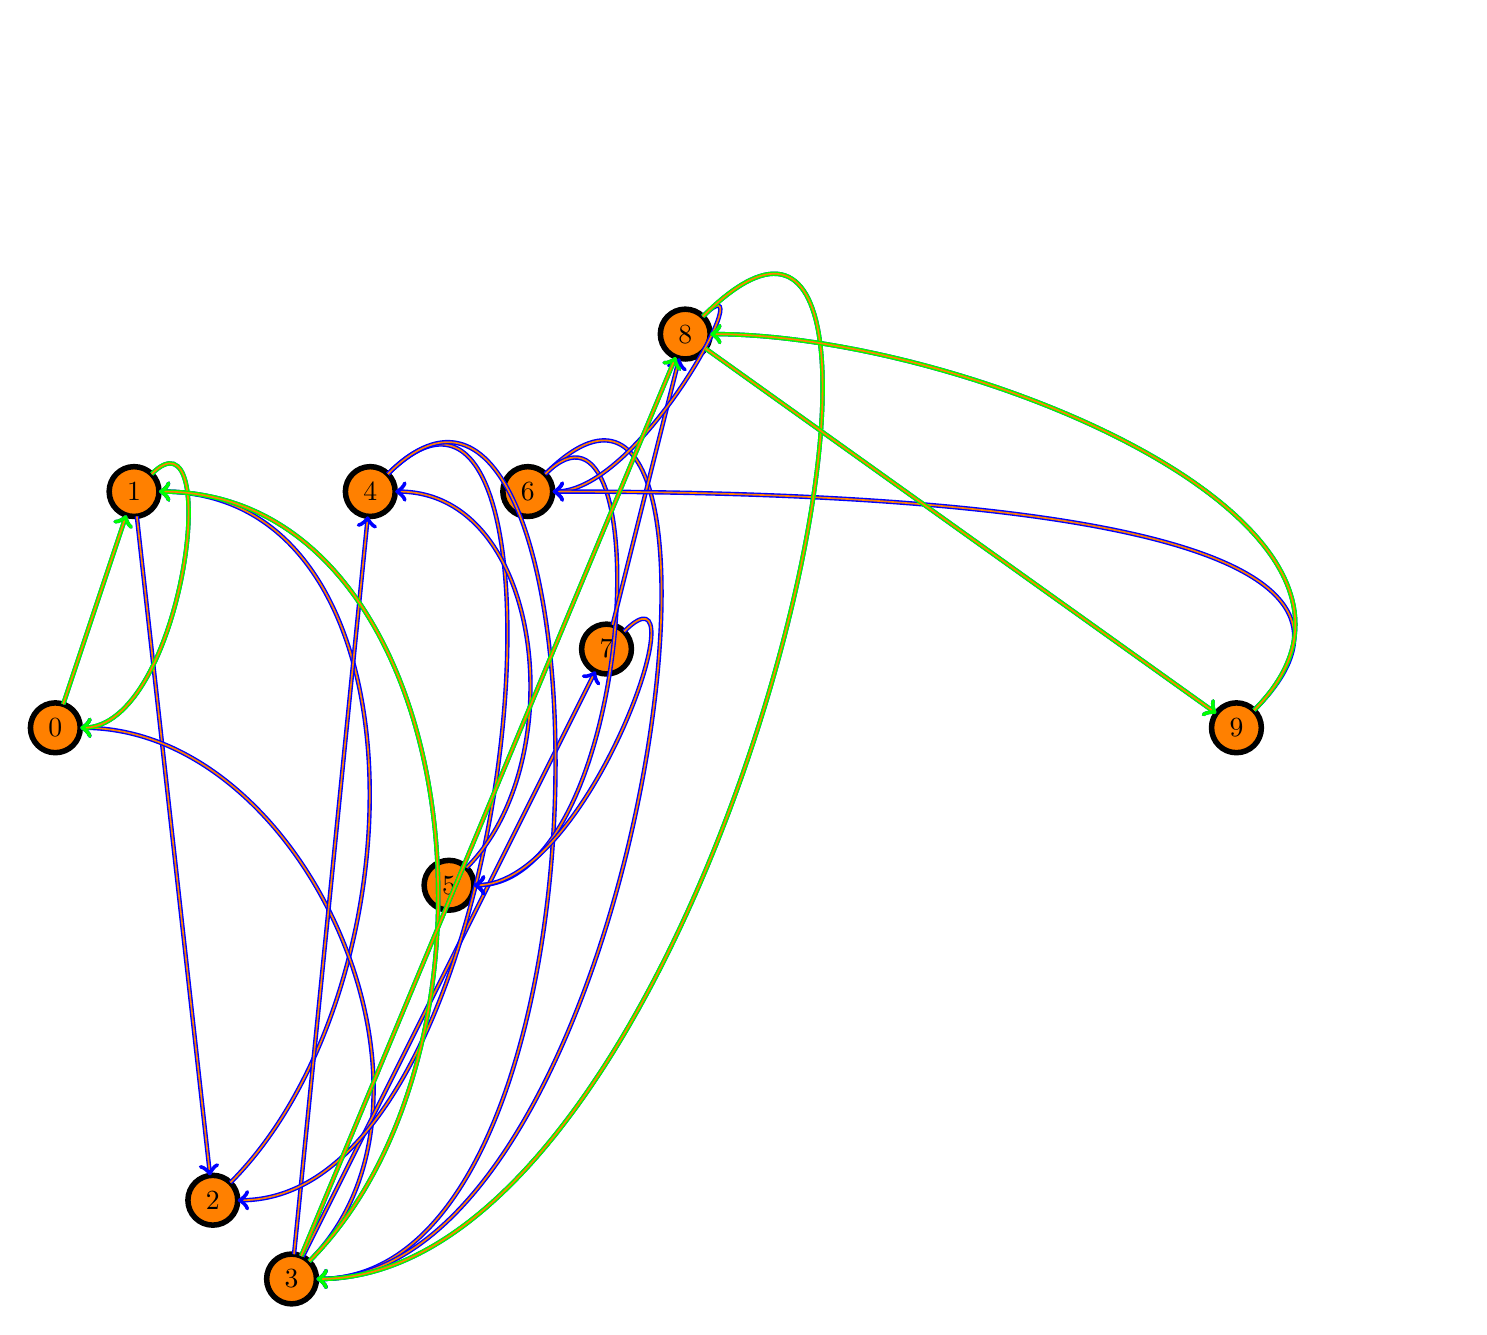
\begin{tikzpicture}
\SetVertexNormal[Shape      = circle,
FillColor  = orange,
LineWidth  = 2pt]
\SetUpEdge[lw         = 0.5pt,
color      = black,
labelcolor = white,
labeltext  = red,
labelstyle = {sloped,text=blue}]
\tikzstyle{TempStyle}=[double = orange]
\Vertex[x=-10, y=8]{0}
\Vertex[x=-9, y=11]{1}
\Vertex[x=-8, y=2]{2}
\Vertex[x=-7, y=1]{3}
\Vertex[x=-6, y=11]{4}
\Vertex[x=-5, y=6]{5}
\Vertex[x=-4, y=11]{6}
\Vertex[x=-3, y=9]{7}
\Vertex[x=-2, y=13]{8}
\Vertex[x=5, y=8]{9}
\tikzset{EdgeStyle/.style={->,TempStyle,relative=false,right=60,color=blue}}
\Edge(0)(1)
\tikzset{EdgeStyle/.style={->,TempStyle,relative=false,left=60,color=blue,in=0,draw}}
\Edge(1)(0)
\tikzset{EdgeStyle/.style={->,TempStyle,relative=false,right=60,color=blue}}
\Edge(1)(2)
\tikzset{EdgeStyle/.style={->,TempStyle,relative=false,left=60,color=blue,in=0,draw}}
\Edge(2)(1)
\tikzset{EdgeStyle/.style={->,TempStyle,relative=false,left=60,color=blue,in=0,draw}}
\Edge(3)(0)
\tikzset{EdgeStyle/.style={->,TempStyle,relative=false,left=60,color=blue,in=0,draw}}
\Edge(3)(1)
\tikzset{EdgeStyle/.style={->,TempStyle,relative=false,right=60,color=blue}}
\Edge(3)(4)
\tikzset{EdgeStyle/.style={->,TempStyle,relative=false,right=60,color=blue}}
\Edge(3)(7)
\tikzset{EdgeStyle/.style={->,TempStyle,relative=false,right=60,color=blue}}
\Edge(3)(8)
\tikzset{EdgeStyle/.style={->,TempStyle,relative=false,left=60,color=blue,in=0,draw}}
\Edge(4)(2)
\tikzset{EdgeStyle/.style={->,TempStyle,relative=false,left=60,color=blue,in=0,draw}}
\Edge(4)(3)
\tikzset{EdgeStyle/.style={->,TempStyle,relative=false,left=60,color=blue,in=0,draw}}
\Edge(5)(4)
\tikzset{EdgeStyle/.style={->,TempStyle,relative=false,left=60,color=blue,in=0,draw}}
\Edge(6)(3)
\tikzset{EdgeStyle/.style={->,TempStyle,relative=false,left=60,color=blue,in=0,draw}}
\Edge(6)(5)
\tikzset{EdgeStyle/.style={->,TempStyle,relative=false,left=60,color=blue,in=0,draw}}
\Edge(7)(5)
\tikzset{EdgeStyle/.style={->,TempStyle,relative=false,right=60,color=blue}}
\Edge(7)(8)
\tikzset{EdgeStyle/.style={->,TempStyle,relative=false,left=60,color=blue,in=0,draw}}
\Edge(8)(3)
\tikzset{EdgeStyle/.style={->,TempStyle,relative=false,left=60,color=blue,in=0,draw}}
\Edge(8)(6)
\tikzset{EdgeStyle/.style={->,TempStyle,relative=false,right=60,color=blue}}
\Edge(8)(9)
\tikzset{EdgeStyle/.style={->,TempStyle,relative=false,left=60,color=blue,in=0,draw}}
\Edge(9)(6)
\tikzset{EdgeStyle/.style={->,TempStyle,relative=false,left=60,color=blue,in=0,draw}}
\Edge(9)(8)
\tikzset{EdgeStyle/.style={->,TempStyle,relative=false,right=60,color=green}}
\Edge(0)(1)
\tikzset{EdgeStyle/.style={->,TempStyle,relative=false,right=60,in=0,color=green}}
\Edge(1)(0)
\tikzset{EdgeStyle/.style={->,TempStyle,relative=false,right=60,in=0,color=green}}
\Edge(3)(1)
\tikzset{EdgeStyle/.style={->,TempStyle,relative=false,right=60,color=green}}
\Edge(3)(8)
\tikzset{EdgeStyle/.style={->,TempStyle,relative=false,right=60,in=0,color=green}}
\Edge(8)(3)
\tikzset{EdgeStyle/.style={->,TempStyle,relative=false,right=60,color=green}}
\Edge(8)(9)
\tikzset{EdgeStyle/.style={->,TempStyle,relative=false,right=60,in=0,color=green}}
\Edge(9)(8)
\end{tikzpicture}\\
\begin{center}\begin{tabular}{l c}\\
\textcolor{orange}{\LARGE$\rightarrow$} & Chemin \\
 \textcolor{red}{\LARGE$\rightarrow$} & Créations arcs\\
 \textcolor{green}{\LARGE$\rightarrow$} & Modification flot\\
\end{tabular}
\end{center}
\end{document}
